% minted: pdflatex: {shell: true}
\documentclass[12pt,letterpaper]{report}
\renewcommand{\contentsname}{Table Of Contents}
\usepackage{indentfirst}
\usepackage{setspace}
\usepackage[margin=1in]{geometry}
\usepackage{eso-pic,graphicx}
\usepackage{apacite} 
\usepackage{amsthm}
\usepackage{amssymb}
\usepackage{amsmath}
\usepackage{subcaption}
\usepackage{tikz}
\usepackage{wrapfig}
\usepackage{lscape}
\usepackage{rotating}
\usepackage{epstopdf}
\usepackage[toc,page]{appendix}
\usepackage{tocloft}
\usepackage[explicit]{titlesec}
\usepackage{float}
\usepackage{physics}
\usepackage{titlesec}
\usepackage{chngcntr}
\usepackage{listings}
\usepackage{color}
\usepackage{longtable}
\usepackage[textfont = it, labelfont = bf, font = small, format = hang]{caption}
\definecolor{mygreen}{rgb}{0,0.6,0}
\definecolor{mygray}{rgb}{0.5,0.5,0.5}
\definecolor{mymauve}{rgb}{0.58,0,0.82}
\definecolor{ao}{rgb}{0.0, 0.0, 1.0}
\definecolor{asparagus}{rgb}{0.53, 0.66, 0.42}

\lstset{ 
	backgroundcolor=\color{white},   % choose the background color; you must add \usepackage{color} or \usepackage{xcolor}; should come as last argument
	basicstyle=\footnotesize,        % the size of the fonts that are used for the code
	breakatwhitespace=false,         % sets if automatic breaks should only happen at whitespace
	breaklines=true,                 % sets automatic line breaking
	captionpos=none,                    % sets the caption-position to bottom
	commentstyle=\color{mygreen},    % comment style
	deletekeywords={np.abs,range},            % if you want to delete keywords from the given language
	escapeinside={\%*}{*)},          % if you want to add LaTeX within your code
	extendedchars=true,              % lets you use non-ASCII characters; for 8-bits encodings only, does not work with UTF-8
	firstnumber=1000,                % start line enumeration with line 1000
	frame=none,	                   % adds a frame around the code
	keepspaces=true,                 % keeps spaces in text, useful for keeping indentation of code (possibly needs columns=flexible)
	keywordstyle=\color{ao},       % keyword style
	language=Python,                 % the language of the code
	morekeywords={*,TRUE,FALSE},            % if you want to add more keywords to the set
	numbers=none,                    % where to put the line-numbers; possible values are (none, left, right)
	numbersep=5pt,                   % how far the line-numbers are from the code
	numberstyle=\tiny\color{mygray}, % the style that is used for the line-numbers
	rulecolor=\color{black},         % if not set, the frame-color may be changed on line-breaks within not-black text (e.g. comments (green here))
	showspaces=false,                % show spaces everywhere adding particular underscores; it overrides 'showstringspaces'
	showstringspaces=false,          % underline spaces within strings only
	showtabs=false,                  % show tabs within strings adding particular underscores
	stepnumber=2,                    % the step between two line-numbers. If it's 1, each line will be numbered
	stringstyle=\color{mygreen},     % string literal style
	tabsize=2,	                   % sets default tabsize to 2 spaces
	title=\lstname                   % show the filename of files included with \lstinputlisting; also try caption instead of title
}

\counterwithout{figure}{chapter}
\counterwithout{table}{chapter}

\setcounter{tocdepth}{4}
\setcounter{secnumdepth}{4}
\usetikzlibrary{arrows.meta, calc, positioning}

\tikzset{flow chart/.style = {
		base/.style = {rectangle, rounded corners, draw, inner sep=2mm, outer sep=0mm},
		startstop/.style = {base, minimum size=15mm},
		second/.style = {base, minimum width=2cm, minimum height=1cm},
		dot/.style = {circle, fill=black, minimum size=1mm,
			inner sep=0pt, outer sep=0pt, node contents={}},
		LA/.style = {thick,-Stealth}
	}
}% end tikzset


\newtheorem{definition}{Definition}
\newtheorem{assumption}{Assumption}
\newtheorem{theorem}{Theorem}
\bibliographystyle{apacite}
\titleformat{\chapter}[display]{\bfseries\centering}{\huge Chapter \thechapter}{1em}{\Huge #1}
\graphicspath{{C:/Users/JM/Google Drive/THESIS/MANUSCRIPT-FINAL/MANUSCRIPT-FINAL}}

\begin{document}
\begin{titlepage}
\begin{center}
	\begin{figure}
	\centering
	\includegraphics[width=6cm]{"DLSU LOGO".png}	
	\end{figure}
	\vspace*{0.25cm}
	\large
	\textbf{Assessing Systemic Risk in the Integrated Circuit \\
	World Trade Network Using Cascading Failure Agent-based Simulations}
	
	\vspace{1cm}
	\normalsize
	An Undergraduate Thesis Submitted to the\\Physics Department\\De La Salle University\\Taft Avenue, Manila
	
	\vspace{1cm}
	\normalsize
	In Partial Fulfillment\\Of the Requirements for the Degree of\\Bachelor of Science in Physics Minor in Economics\\
	\vspace{1cm}
	\normalsize
	by\\
	Justin Gabrielle A. Manay\\
	\vspace{0.5cm}
	\normalsize
	Adviser\\
	Rene C. Batac, Ph.D.\\
	\vspace{0.5cm}
	\normalsize
	April 2020
	\vfill
\end{center}
\end{titlepage}
\newgeometry{left=1.3in, right=1.13in, top=1.88in,bottom=1.45in}
\AddToShipoutPictureBG{\includegraphics[width=\paperwidth,height=\paperheight]{"thesisbackground".jpg}}

\section*{\centering Approval Sheet}
\begin{flushleft}
	This thesis proposal hereto entitled:
\end{flushleft}
\begin{center}
	\underline{ \hspace{0.43in}Assessing Systemic Risk in the Integrated Circuit
	\hspace{0.41in}} \\
	\vspace{0.5cm}
	\underline{\hspace{0.15in}World Trade Network Using Cascading Failure Agent-based Simulations \hspace{0.10in}}
\end{center}
prepared and submitted by \underline{Justin Gabrielle A. Manay} in partial fulfilment of the requirements for the degree of
	\begin{center}
		\underline{\hspace{0.5in} Bachelor of Science in Physics Minor in Economics \hspace{0.5in}}
	\end{center} 
has been examined and is recommended for acceptance and approval for ORAL EXAMINATION. 

\begin{flushright}
	\begin{tabular}{@{}p{.5in}p{2.5in}@{}}
		& \quad \quad \quad   Rene C. Batac, Ph.D.\\
		& \hrulefill \\
		& \quad \quad \quad \quad \quad \quad Adviser \\
	\end{tabular}
	\\
\end{flushright}


\begin{flushleft}
Approved by the Committee on Oral Examination with a grade of PASSED on\\
\end{flushleft}
\makebox[1in]{\hrulefill}

\begin{center}
	\begin{tabular}{@{}p{.5in}p{2.5in}@{}}
		& \quad \quad \qquad   \\
		& \hrulefill \\
		& \quad \quad \quad \quad \qquad  Chair \\
	\end{tabular}
	\\
	\begin{tabular}{@{}p{.5in}p{2in}@{}@{}p{.5in}p{2in}@{}}
		& \quad \quad \qquad  && \quad \quad \qquad \\
		& \hrulefill && \hrulefill\\
		& \quad \quad \quad \quad  Member && \quad \quad \quad \quad  Member\\
	\end{tabular}
	\\
\end{center}


\begin{flushleft}
	Accepted in partial fulfilment of the requirements for the degree of \\
\end{flushleft}


\begin{center}
\underline{\hspace{0.5in} Bachelor of Science in Physics Minor in Economics \hspace{0.5in}}
\end{center} 

\begin{flushright}
\begin{tabular}{@{}p{.5in}p{2.5in}@{}}
	& \quad \quad \quad  \\
	& \hrulefill \\
	& \quad \quad \quad \quad \quad \quad Dean \\
	& \quad \quad \quad College of Science \\
\end{tabular}
\end{flushright}
\pagebreak

\section*{\centering Abstract}
	\noindent
	 Network analysis allows us to simulate economic shocks in order to examine their effects on all the other countries in the trade network. In light of this, this paper aims to characterize the integrated circuit (IC) trade network by employing a three-part analysis, which involves: (i) characterizing the network using network measures, such as link density and total link weight, (ii) using centrality measures to determine key nodes in the network, and (iii) employing the cascading failures model to propagate economic shocks in the network, then using cascade-based measures to identify key nodes and possibly characterize the underlying structure of the network. We found that the link density and total link weight have largely been increasing over the years, primarily due to globalization. The agent-based simulation also revealed that the both the network of outgoing and incoming links exhibit a core-periphery structure. That is, the IC trade networks are characterized by a highly central and well-connected core and a sparsely-connected periphery. This allowed us to earmark core countries, which are more likely to be subject to systemic risk. Notably, we found that there are three main (geographic) blocs for the IC network: North America, Western Europe and East/Southeast Asia, which are primary intermediary hubs in the IC network. As such, the three regions pose a significant systemic risk, as they are not only important exporters but are important importers as well. 


\section*{\centering Acknowledgment}
\noindent I would like to extend my sincerest thanks to my thesis adviser Rene C. Batac, Ph.D. for his guidance throughout the entire thesis process and for inspiring me to further explore the field of complex systems and quantitative social science in the future.

\pagebreak

\tableofcontents
\pagebreak
 
\listoffigures
\pagebreak

\listoftables
\pagebreak

\section*{Glossary of Terms}
\begin{longtable}{|p{5cm}|p{8cm}|}
	\caption{Important terms used in the paper and their definitions.} \\
	\hline
	\textbf{\small Term} & \textbf{\small Definition} \\
	\hline
	\endfirsthead
	\hline
	\textbf{\small Term} & \textbf{\small Definition} \\
	\hline
	\endhead
	integrated circuit (IC) & Collectively refers to all products traded with ID 8542 under the HS92 scheme. This is the name of the commodity under investigation. \\
	\hline
	IC trade network & The trade network formed by all countries that are engaged in integrated circuit trade. The network is unilateral, with the weights being net exports. \\
	\hline
	network analysis & Not to be confused with circuit analysis, this refers to the empirical study of networks, such as trade networks. \\
	\hline
	node & Refer to the basic units in the network. In the trade network, nodes represent the individual countries. \\
	\hline
	edge & Refer to the connections or links between nodes. In the trade network, edges represent the links between countries. \\
	\hline
	(un)directed network & Undirected networks have directionless edges. Directed networks are those whose edges are associated with a certain direction. \\
	\hline
	bilateral/unilateral network & A bilateral network is one where there can be two edges (to and from each node) between any two nodes. In a unilateral network, there can only be one edge between any two nodes.  \\
	\hline
	weight & Refer to attributes that are associated with the edges. In the trade network, these are the net exports between countries \\
	\hline
	centrality & Generally refers to the importance of a node in a network. \\
	\hline
	rank-size distribution & Refers to a distribution where the quantities are plotted against their ranks, usually in descending order. \\
	\hline
	degree & Refers to the number of edges that are adjacent to a node. It can be decomposed into in-degree (number of edges pointing into a node) and out-degree (number of edges pointing out of a node) \\
	\hline
	strength centrality & Weighted analogue of degree centrality. It can be decomposed into in-strength and out-strength. \\
	\hline
	shortest path & Also known as geodesic distance, it is the shortest sequence of nodes (each connected to the previous one by an edge) from an origin to a destination where no node repeats itself. \\
	\hline
	betweenness centrality & Refers to the percentage of all shortest paths that pass through a given node. It quantifies how "in-between" a node is in the network in general. \\
	\hline
	eigenvector centrality & Generally quantifies how important a node is, taking into account how important its neighbors are. It can be decomposed into in-eigenvector and out-eigenvector. \\
	\hline
	density & Refers to the propotion of edges present in the network out of the number of possible edges. This quantifies how well-connected a network is in general. \\
	\hline
	(degree) assortativity & Generally quantifies how preferential the attachment is between nodes of similar classes (i.e., Do nodes of high degree tend to link with other nodes of high degree?) \\
	\hline
	core-periphery structure & Network structure with well-connected core nodes and sparsely-connected peripheral nodes. The core in this network structure has been found to be susceptible to systemic risk. \\
	\hline
	systemic risk & Refers to the
	risk of collapse of any system due to events at the individual level. \\
	\hline
	agent-based simulation & A computational model that simulates the interaction of multiple agents with each other in light of viewing their effect on the entire system. \\
	\hline
	economic shocks & In this study, we will limit the economic shocks to supply-side perturbations (i.e., increase or decrease). \\
	\hline
	cascading failures model & Model where the failure of one node "cascades" to all other adjacent ones in the network. This is used to model systemic risk. \\
	\hline
	shock parameter & In the model, this parameterizes the percent decrease in a country's total exports/imports due to a supply-side decrease/increase, respectively. \\
	\hline
	spread parameter & In the model, this parameterizes the percent of the shock that is propagated to a country's export/import partners in the case of a supply-side decrease/increase, respectively. \\
	\hline
	cascade size & Refers to the number of unique edges affected by the cascade. \\
	\hline
	cascade depth & Refers to the number of iterations it takes before the cascade terminates. \\
	\hline
	exposure & Refers to the percent of initial shock absorbed by a particular country.\\ 
	\hline
	minimum shock & Refers to the minimum amount of the shock parameter needed to designate a node in the network as a core node, setting the spread parameter to 1. The definition of a core node in the network under consideration is heuristic and will be determined from simulation data.\\ 
	\hline
\end{longtable}
\pagebreak

\spacing{1.5}

%-----------------------------
% CHAPTER 1
%-----------------------------
\chapter{Introduction}
\label{chap:1Intro}

This chapter presents the research and its rationale. It consists of the background and motivation of the study, its general and specific objectives, the scope and delimitation of the study, and the significance of the study.

%-----------------------------
% Section 1.1
%-----------------------------
\section{Background and Motivation of the Study}
\label{sec:11Background}
	 
	 Trade literature on the Philippines has primarily focused on the gravity model of trade, which presupposes that trade volume is a function of the gross domestic product (GDP) of the trading countries and the geographical distance between them. In particular, the gravity model assumes that the trade volume $T_{ij}$ between two countries $i$ and $j$ with GDPs $Y_i$ and $Y_j$  and geographical distance $d$ is given by
	 
\begin{equation}
\label{eqn:c01Tij} T_{ij} = A \frac{Y_i^{\beta_1}Y_j^{\beta_2}}{d} u_{ij}
\end{equation}
	 
\noindent where $A$ is a constant and $u_{ij}$ is an error factor. Equation~(\ref{eqn:c01Tij}) can be re-expressed as 

\begin{equation}
\label{eqn:c02Tij} \ln T_{ij} = \ln A + \beta_1 \ln Y_i + \beta_2 \ln Y_j - \ln d + \ln u_{ij}
\end{equation}

	Note that equation~(\ref{eqn:c02Tij}) is a linear function, which can be conveniently estimated through ordinary least squares regression \cite{reinert2011introduction}.
	
	This model tells us how trade volume varies with the given variables on average. However, it fails to give us any insight on how trade shocks can propagate through the international economy. As such, the results of analyses using gravity trade models, while generalizable, are not immediately useful in the realm of policy analysis.
	
	It helps to view international trade as a set of complex relationships between countries. This allows us to simulate economic shocks by tweaking particular variables so as to observe their repercussions on the trade network in general. This is especially important in this era of supply shortages, economic sanctions and trade wars. 
	
	Thus, network analysis provides us with a new lens through which we can view not only bilateral trade but inter-country relationships in general \cite{bowen1998applied}. The wealth of data from the World Trade Organization, the World Bank and various trade blocs like the Association of Southeast Asian Nations (ASEAN), the Asia-Pacific Economic Community (APEC) and the European Union (EU), among others, lends credence to employing this particular approach in trade analysis. Some databases even offer trade flow data at a more granular level, allowing us to examine trade networks for particular commodity groups such as crops \cite{burkholz2019international}, bananas, cement, oil and others \cite{de2014network}. 
	
	Moreover, network analysis also allows us to assess the systemic risk inherent in the trade network. Certain structures like the core-periphery structure are more vulnerable to systemic risk. Using network analysis, we can identify the existence of a core-periphery structure and correspondingly determine which nodes are more susceptible to failures that will likely end up upending the entire network.
	
	As such, network analysis provides us with an attractive set of tools that can help shed light on the Philippines’ place in the world trade network.
	 
%-----------------------------
% Section 1.2
%-----------------------------
\section{Objectives of the Study}
\label{sec:12Objectives}

%-----------------------------
% Subsection 1.2.1
%-----------------------------
\subsection{General Objective}
\label{ssec:121GenObj}
		
		This paper aims to characterize the integrated circuit trade network by employing a three-part analysis, which involves: (i) characterizing the network using known measures, such as link density, total link weight and degree assortativity; (ii) using centrality measures to determine key nodes in the network, with emphasis on the Philippines’ possible role in the trade network and (iii) employing the cascading failures model to propagate economic shocks in the network, then using cascade-based measures to identify key nodes and possibly characterize the underlying structure of the network. 
		
%-----------------------------
% Subsection 1.2.2
%-----------------------------
\subsection{Specific Objectives}
\label{ssec:122SpecObj}
		
		In particular, the study aims to accomplish the following:
		
		\begin{itemize}
		
		\item [1.] determine key characteristics of the integrated circuit trade network and how they change over time. The trade network will be constructed based on UN data and as such, it will exclude disputed/unrecognized territories like Taiwan/Chinese Taipei and Kosovo.
		
		\item [2.] identify key nodes in the network based on centrality measures
		
		\item [3.] employ agent-based simulation to propagate various economic shocks in the trade network using the cascading failures model
		
		\item [4.] use cascade-based measures to identify key nodes in the network
		
		\item [5.] characterize the structure of the network based on the results of the cascades
		
		\end{itemize}
		
%-----------------------------
% Section 1.3
%-----------------------------
\section{Scope and Delimitation}
\label{sec:13Scope}
	
	This paper will simply focus on the integrated circuit trade network. This choice was made in light of the Philippines being a key exporter and importer of integrated circuits based on the Observatory of Economic Complexity \cite{simoes2011economic}. Based on 2017 data, integrated circuits constitute the largest share of the country's exports and imports, accounting for 32\% of the country's exports and 11\% of the country's imports. 
	
	The trade networks will be constructed on the basis of data from UN Comtrade. As such, certain territories (e.g., Taiwan/Chinese Taipei, Kosovo) that are presently not recognized by the UN or were not recognized during the time frame chosen will thus be excluded due to lack of data. 
	
	Initially, we will construct bilateral trade networks using trade data from the UN Comtrade database for the years 2013-2017. For reasons to be discussed later on in the paper, we will convert these into unilateral networks based on the net weight. Thus, the computed network-level and node-level measures will apply to these unilateral networks. The network-level measures to be computed will include link density, total link weight and degree assortativity. The node-level measures will be limited to the degree, strength, betweenness and eigenvector centrality. Moreover, the agent-based simulation of economic shocks, as outlined in Chapter 3 of the paper, will apply to the unilateral networks earlier described. 
	
	All the analysis and visualizations will be conducted using the NetworkX package in Python.
	
%-----------------------------
% Section 1.4
%-----------------------------
\section{Significance of the Study}
\label{sec:14Significance}
	
	While there have been many studies on the world trade network, literature specific to the integrated circuits and to the Philippines in particular remain relatively scant. Most of the existing studies simply analyze the Philippines' trade flows with other countries in isolation, failing to take into account the dependence of these flows on other trade flows in the trade network. A US embargo on China, for example, may lead to China increasing its trade flows with its neighbors. Network analysis allows us to integrate these network effects into the analysis.
	
	The network approach also gives us a tool to simulate how certain economic shocks not specific to the Philippines can propagate through the network and potentially affect the country. This is particularly useful for policy analysts as it provides them with a model for crisis management.
	
	The study can also be used to gain insight on the Asia-Pacific region’s and the Philippines' place in the trade network and reveal data regarding its comparative advantage relative to other similar countries in the trade network. While this data may already be probably known already, network analysis provides us with a new avenue to gauge this comparative advantage so that we know how much leverage the country has in trade deals with other countries.
	
%-----------------------------
% CHAPTER 2
%-----------------------------
\chapter{Review of Related Literature}
\label{chap:2Review}

	This chapter presents summaries of research that are related to this study. This section is divided into three sections, discussing literature regarding the (1) characterization of world trade networks and (2) propagation of economic shocks.
	
%-----------------------------
% Section 2.1
%-----------------------------	
\section{Characterization of World Trade Networks}
\label{sec:21Characterization}

	Serrano and Boguñá (2003) were one of the first researchers to perform an empirical characterization of the topology of the world trade network, examining 179 countries during the year 2000. They found that the weighted link distribution is heavily right-skewed. Furthermore, they found that the world trade network exhibited reasonably high reciprocity (i.e., many bidirectional links), an ``income'' effect, in which countries with higher per capita GDP are associated with more links and a relatively small average distance.	

	In a later study, Serrano, Boguñá \& Vespignani (2007) constructed a world trade network for years 1948 to 2000, weighting the relationships between trade partners using their trade imbalance (defined as exports minus imports). They characterized the topology of the resulting network by using basic metrics such as the in-degree ($k_{in}$), out-degree ($k_{out}$), in-strength ($s_{in}$) and out-strength ($s_{out}$), among others. They were also able to get the total flux of money leaving or entering a country due to trade by summing the weights of the incoming and outgoing links, respectively. Through this, they were able to characterize certain countries as net consumers and net producers.
	
	As in their previous study, they found that the resulting probability distribution of the flux exhibited heavy-tailed behavior, suggesting that there were only a few particularly important links in the network. By constructing a null model for the normalized link fluxes, they were able to filter out the most dominant ones by statistical analysis. Through this, they were able to examine the evolution of dominant flows across time, noting in particular the lack of strong trade relations between the opposing blocs during the Cold War, the emergence of the US, Japan and China as powerful trading hubs and the wane in influence of other countries such as the UK.
	
	Fagiolo, Reyes \& Schiavo (2010) used a 159-country dataset for the years 1981 and 2000, constructing an export trade network in which the links are weighted by normalized exports (exports divided by the GDP of the exporting country). They performed an undirected network analysis in light of discrepancy in the values reported by the exporting and importing countries, although such an analysis is justified by the high reciprocity of the world trade network \cite{serrano2003topology}. They found that world trade networks tend to be extremely dense and that while the unweighted link distribution is homogeneous (and bimodal), the weighted link distribution exhibits heavy right-skewness, as in Serrano \& Boguñá (2003). They also found negative assortativity coefficients. Lastly, comparing the world trade network during the two years studied, most of the structural properties of the trade network tend to be stationary, with primarily the density and reciprocity increasing due to globalization. In general, they found that the world trade network is characterized by a relatively high network density and has a higher node strength, assortativity coefficient, clustering coefficient and random walk betweenness centrality than comparable random graphs, signifying that on average, the world trade network is more clustered, more assortative and has nodes which are more central compared to comparable random graphs.
	
	Barigozzi et al. (2010) used Comtrade data for 162 countries during the 1992-2003 period to construct 97 commodity-specific networks. Comparing the commodity-specific networks with the aggregate network, they found that the unweighted links were more homogeneously distributed while links in the commodity-specific networks were rather heterogeneously distributed, suggesting that the world trade network is itself a complex system. The density and reciprocity are also higher for the aggregate network, supporting this claim.
	
	De Benedictis et al. (2014) studied 178 countries during the years 1995 to 2010 utilizing the BACI-CEPII dataset, which reconciles the discrepancy in values between exporting and importing countries. Instead of using a country's geographical position to represent its place in the world trade network, they emphasized the use of a sociogram, which uses a force-directed algorithm, to determine the visualization. This results in connected countries being closer to each other and disconnected countries being farther apart in the visualization, highlighting the conditional interdependence of bilateral trade flows.
	
	As before, they found that the world trade network had become increasingly dense, and the weighted links had exhibited even more heterogeneity – a heavy right-skewed distribution, in particular. In fact, they found that world trade is governed primarily by 17 core countries, with the remaining countries in the periphery.
	
	Cepeda-López et al. (2019) constructed 16 commodity-specific export networks from 1995-2014 using Comtrade data. In agreement with previous studies, they found that the export networks are increasingly dense but that links were more intense in past than in later years, what with the rise of other countries like China and Hong Kong as dominant exporters. In concert with the increase in density, the mean geodesic distance decreased over time, while the reciprocity and clustering coefficient increased. 
	
	Unlike Reyes, Fagiolo \& Schiavo (2010), they found positive assortativity coefficients, sorting by both degree and strength. Also, as opposed to the previous studies, they found the degree distribution to be weakly left-skewed and the strength distribution to be heavily right skewed. The former is in tune with the increasing density of the world trade network over time.
	
	Overall, they found that the world trade network is dense, reciprocal, compact (i.e., low average distance), clustered, assortative and homogeneous by degree but inhomogeneous strength. Disaggregating the network by sectors, they found different results per sector, again highlighting the complexity inherent in world trade networks.
	
	Characterizing trade network topology through centrality measures can also be used to examine trade integration in a region. Beaton, et al. (2017) used the network approach to characterize economic integration in the Latin American and Caribbean region. They first constructed a bilateral world trade network for 184 countries from 1948 to 2015, classifying the countries into 7 different regions: North America, Latin America, Caribbean, Europe, MENA, Africa and Asia. They found that the Latin American region has trade links with around 70\% of the remaining countries, making the region above average in terms of market diversification. However, using average strength centrality as a measure of economic integration, they found that the Latin American region lags behind other regions, in part because of weak trade flows relative to the economy.
	
	Moreover, while the Latin American region has the densest regional network, there are no strong hubs in the region, as the eigenvector and betweenness centrality measures for the Latin American trade network are only marginally higher than those for the world trade network. These suggest that Latin American trade tends to be concentrated outside of the region, primarily because of strong trade links to the US. This is evidenced by the trade ``communities'' identified in the world trade network using the walktrap algorithm, one of which includes North and Latin America, as well as Cuba and Jamaica in the Caribbean.
	
	Another study which uses centrality measures to characterize trade integration is Nguyen, Pham and Vallée (2016). In particular, they used degree, strength, eigenvector and authority/hub centralities to describe the roles of the countries in the ASEAN+3 region (ASEAN, China, Japan and South Korea). In contrast with Beaton et al. (2017), they compare centralities among countries and not among regions.
	
	They found that China, Japan, South Korea and Singapore have the highest strength centrality in the ASEAN+3 network, signifying that they are the most integrated into the regional trade network. Moreover, while China and Japan rank highly in terms of in-degree, they rank relatively poorly in terms of out-degree. This suggests that China and Japan mainly import from ASEAN but export mainly to other countries outside the region. This is in contrast with countries like Singapore and Brunei, which are important exporters to the region. The important roles of China, Japan, South Korea and Singapore in the region are further highlighted by their relatively high eigenvector centralities. 
	
	For bilateral trade data, a high hub index denotes that a country is a key exporter, while a high authority value means that it is a key importer. Using hub and authority indices, they find that the four countries have the highest values. However, from the earlier results, Japan, China and South Korea are important hubs outside the ASEAN region, while Singapore is an important hub within the region. In contrast, Japan, China and South Korea are key importers, having higher authority indices. As for the other countries in the region, the Philippines, Malaysia, Vietnam and Brunei are key importers (having a higher hub centrality), while the remaining countries have a more symmetric role.
	
	Overall, while China, Japan and South Korea have traditionally dominated trade in the ASEAN+3 region, the region has seen increasing integration, with more peripheral countries like the Philippines, Vietnam and Cambodia becoming more connected to the trade network over time. 

%-----------------------------
% Section 2.2
%-----------------------------		
\section{Propagation of Economic Shocks}
\label{sec:22Shocks}
	
	Serrano, Boguñá and Vespignani (2007) authored one of the first papers to toy with the idea of diffusion in the world trade network. Using their network of trade imbalances during the years 1948-2000, they performed a ``dollar experiment'' in which they run a series of random walk processes on the network. In the first case, they injected one dollar into a consumer country, which then travels through the outgoing links with a probability proportional to the weights associated with them, or gets absorbed by a producer country with some probability Through several repetitions, they were able to calculate the probability $e_{ij}$ that a dollar from source country $i$ finally gets absorbed in sink country $j$.
	
	The second case is symmetric, and involved a producer country receiving a dollar, which then travels through the incoming links with a probability proportional to the weights, or gets retained by a consumer country with some probability. Again, they were able to calculate the probability $g_{ij}$ that a dollar from the source country $i$ finally gets retained in sink country $j$. Through this experiment, they were able to determine where the money spent by consumer countries and the money received by producer countries had been going to and coming from, respectively.
	
	More recent models on trade shocks draw heavily from the cascading failures model of Motter \& Lai (2002). The model applies to networks whose nodes pass loads to other nodes, such as in a power transmission grid. If the load on one node increases to the point of exceeding capacity, the node can fail, leading to the redistribution of loads and the potential for more failure further down the line. In general, they find that cascades occur if (1) the distribution of loads is heterogeneous and (2) the failed node is associated with higher loads than usual. Earlier studies have found a heavily right-skewed distribution for strength centralities, suggesting that load distributions are also heavily heterogeneous. Furthermore, this highlights that certain nodes in the network trade more frequently and in larger volumes than others. Thus, trade networks are heavily susceptible to cascades as in Motter \& Lai's (2002) model. As such, a number of studies have employed the cascading failures model to simulate trade shocks.
	
	One such study is Burkholz \& Schweitzer (2019). They constructed trade networks with respect to different crops from years 1992 to 2013 and then assessed the impact of shocks, which are modelled in the form of one-time exogenous reduction shocks. 
	
	In their model, a supply-side shock is triggered in some country, resulting in a demand deficit. As a result, the country must reduce its exports in such a way that the demand deficit disappears. This reduces the imports of some country, creating a demand deficit which it will then try to reduce in the next time step. Thus, the supply-side shock cascades through the network, until a country can no longer reduce its exports to compensate for the demand deficit.
	
	To systematically study the effects of the cascade on the crop trade network, they considered two different types of shocks: an equal shock, which results in a fixed demand deficit for the shocked country, or a proportional shock, where the deficit depends on the production output of the country. These are separately observed to see how different types of deficits affect the countries in the trade network. This model was run with every possible country as the target of the shock for every possible crop trade network. To visualize the results, they used a higher-order trade dependency network. In particular, they found that a great number of Asian and African countries were most vulnerable to cascades, with the main suppliers of crops being the US, Canada, Argentina, Brazil and India.
	
	Moreover, they found that proportional shocks emphasized the importance of the biggest crop producers, while equal shocks highlighted dependencies between countries. As an example, for the maize network, using proportional shocks revealed the impact of major crop producers such as the US, Brazil and Argentina. Meanwhile, employing equal shocks revealed the role of European countries as intermediaries (i.e., countries that import, add value and export).
	
	A student paper from Loser \& Segel (n.d.) employed the same cascade-based model to examine the impact of country-level shocks to economic growth and to the trade network as a whole for the years 1961 to 2012. In a similar vein to Burkholz \& Schweitzer (2019), they triggered an economic shock to the trade network by sending an impulse to one or more countries in the graph, in the form of a sudden decline in exports. 
	
	Instead of affecting the country's export partners as in Burkholz \& Schweitzer (2019), however, they posited that such an economic shock should lead to a reduction in imports for the affected country, as the decline in exports will reduce national income and lead to less money to spend on imports. This shock then propagates to the affected country's import partners, and is then transmitted to these country's trading partners until the simulation terminates.
	
	They considered two cases: (1) with the transmitted shock being proportional to the decline in exports and (2) with the transmitted shock scaling inversely with the receiving country's imports-to-GDP ratio. The second variation is to account for country-specific responses to the shock. A more closed off country, for example, should have a lower imports-to-GDP ratio and the propagation of trade shocks for such a country should reasonably be small in magnitude. 
	
	To measure the impact of a shock to each node on the network, they analyzed the total cascade size produced by 1\% GDP shocks for each individual node relative to the aggregate GDP. They used this as a measure of node importance and tracked this for all trade networks from 1961 to 2009 to examine how node importance evolves over time. For every trade network from 1961 to 2009, they also triggered a simultaneous 1\% GDP shock at every node to simulate the impact of a coordinated global shock and compared the final cascade impact to the aggregate initial shock over time as a measure of the sensitivity of the trade network to a cascade emanating from a coordinated global shock.
	
	Ultimately, they found that the more well-connected and open a country is, the more susceptible it is to a trade shock. They had also been able to properly simulate an increase in sensitivity during recession periods and the important role of the United States and China in the world trade network.
	
	Gephart et al. (2016) constructed a global trade network for seafood from 205 reporting countries grouped into 18 regions for the year 2011. As in the previous two papers, perturbations are in the form of a decrease in fish exports in one region. These shocks then decrease the flow of imports to other regions. In this model, however, affected regions respond in two ways: (1) reducing exports to other regions, resulting in the propagation of the trade shock, or (2) reducing their domestic consumption and absorbing the shock. 
	
	How much exports to other countries are reduced and how much domestic consumption is reduced both depend on several factors, including but not limited to the volume of exports already in place, local price sensitivity of seafood due to reduced supplies, and the availability of substitute goods. To account for substitutability, they decreased the percent of the shock being transmitted at every iteration. Meanwhile, to account for price sensitivity, they used a willingness-to-pay proxy that is dependent on a region's per-capita-GDP, reflecting the fact that high-income countries tend to be less price-sensitive (because they are more willing to pay) and are thus more likely to pass the shock on to other countries. Low-income countries, on the other hand, are more price-sensitive and are likely to absorb the shocks instead of passing them on.
	
	They ran this model for a range of parameter values and then measured the exposure of a region to the cascade as a percent of initial shock ending up in a region, averaging across all values for the degree of shock, degree of spread, willingness-to-pay proxy and perturbed region. 
	
	They found that a region's exposure increases if it imports more and if it imports from more regions after regressing average exposure with gross imports and the number of regions imported from. This is further evidenced by West Africa, Eastern Asia and Southern and Western Europe being the most exposed regions. They also found that the largest supply decreases occur due to shocks in Northern Europe, Eastern Asia and Southeast Asia, implying that these regions have the most influence in the trade network.
	
	They also found that by increasing the willingness-to-pay proxy parameter, the poorest countries absorbed more of the shock compared to richer countries. Thus, because of relatively high exposure and relatively high price sensitivity, they found that Central and West Africa were the most vulnerable to seafood shocks.

%-----------------------------
% CHAPTER 3
%-----------------------------
\chapter{Framework of the Study}
\label{chap:3Framework}

This chapter consists of the theoretical background of the study. This chapter is divided into three sections: (1) basics of network analysis, (2) core-periphery structures in networks and (3) shock propagation in trade networks.

%-----------------------------
% Section 3.1
%-----------------------------
\section{Basics of Network Analysis}
\label{sec:31Basics}

%-----------------------------
% Subsection 3.1.1
%-----------------------------
\subsection{Introduction to Networks}
\label{ssec:311Intro}

	A \textit{network} is simply a collection of nodes (or vertices) joined together by edges (or links). Mathematically, they are often represented by graphs, which are denoted by the tuple $G = (V,E)$ where $V$ is the set of all nodes and $E \in V \times V$ is the set of all edges linking these nodes. If the elements of $E$ are ordered pairs (that is, if the edges have a direction pointing from one node to another), the graph is \textit{directed}, whereas if they are unordered, the graph is \textit{undirected}. Edges can also be associated with a weight, which describes the intensity of the relationship between the two nodes.
	
	Networks are often described by an \textit{adjacency matrix} $A$, which is an $N \times N$ matrix ($N$ being the number of nodes in the network), such that the element $A_{ij}  = 1$ if an edge exists from node $i$ to node $j$ and $A_{ij}  = 0$ otherwise. This means that the adjacency matrix must be symmetric for undirected networks and asymmetric for directed ones. 

\begin{figure}[!h]
\centering
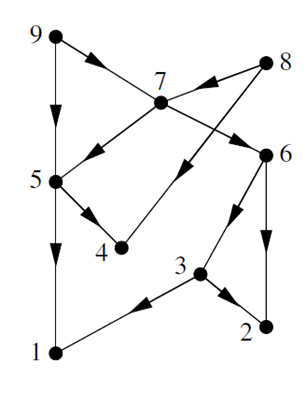
\includegraphics[width=0.3\columnwidth]{Fig301-Network.png}
\caption{An example of a network from Newman (2018).}\label{fig:301Network}
\end{figure}
	
	To illustrate this, we use a network from Newman (2018) as an example, shown in Figure \ref{fig:301Network}. The associated adjacency matrix A for such a network would be as follows:

\begin{equation}
\label{eqn:301A} A = 
\begin{pmatrix}
0 & 0 & 0 & 0 & 0 & 0 & 0 & 0 & 0 \\
0 & 0 & 0 & 0 & 0 & 0 & 0 & 0 & 0 \\
1 & 1 & 0 & 0 & 0 & 0 & 0 & 0 & 0 \\
0 & 0 & 0 & 0 & 0 & 0 & 0 & 0 & 0 \\
1 & 0 & 0 & 1 & 0 & 0 & 0 & 0 & 0 \\
0 & 1 & 1 & 0 & 0 & 0 & 0 & 0 & 0 \\
0 & 0 & 0 & 0 & 1 & 1 & 0 & 0 & 0 \\
0 & 0 & 0 & 1 & 0 & 0 & 1 & 0 & 0 \\
0 & 0 & 0 & 0 & 1 & 0 & 1 & 0 & 0 \\
\end{pmatrix}
\end{equation}

	Weighted networks are often associated with a weight matrix $W$ where the values $W_{ij}$  are the weights associated with the edges.
	
	A node $i$ is often described by its degree $k_i$ which is the number of edges connected to it. This is given by:

\begin{equation}
\label{eqn:302Degree} k_i = \sum_{j=1}^{N} A_{ij}
\end{equation}	

	In directed networks, it is useful to make the distinction between a node's in-degree and out-degree. For node $i$, the in-degree is the number of incoming edges connected to it, while the out-degree is the number of outgoing edges connected to it. These are given by:

\begin{equation}
\label{eqn:303InDegree} k_i^{in} = \sum_{j=1}^{N} A_{ij}
\end{equation}	

\begin{equation}
\label{eqn:304OutDegree} k_i^{out} = \sum_{j=1}^{N} A_{ij}
\end{equation}	

	The analog of the degree for weighted networks is the \textit{strength}, and is computed similarly as in equations ~(\ref{eqn:302Degree}) to ~(\ref{eqn:304OutDegree}) except using the weight matrix associated with the network.
	
	It is often instructive to construct a \textit{probability distribution} to determine the frequency with which particular values of the degree appear in the network. We again refer to an example from Newman (2018) to illustrate the idea of the degree and the degree distribution (i.e., the probability distribution for the degree), as shown in Figure\ref{fig:302NetworkDegree}. 

\begin{figure}[!h]
\centering
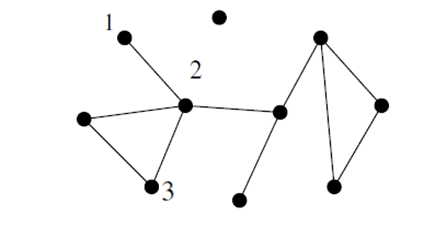
\includegraphics[width=0.5\columnwidth]{Fig302-NetworkDegree.png}
\caption{An example of a network for illustrating degree distributions from Newman (2018).}\label{fig:302NetworkDegree}
\end{figure}	
	
	The network in Figure\ref{fig:302NetworkDegree} has 10 nodes. We can see that node 1 has a degree of 1, node 2 a degree of 4 and node 3 a degree of 2. Going further, we can calculate the degree for all 10 nodes and let $p_k$ denote the fraction of nodes with degree $k$. Proceeding with this calculation, we find that 
	
\begin{equation}
\label{eqn:305DegreeDistribution} p_0 = \frac{1}{10} \textrm{, } p_1 = \frac{2}{10} \textrm{, } p_2 = \frac{4}{10} \textrm{, } p_3 = \frac{2}{10} \textrm{, } p_4 = \frac{1}{10}
\end{equation}

	The set  $\left\{p_i\right\}_{i=0}^{4}$ represents the degree distribution of the network, which can be visualized by plotting the values on a histogram. Empirically, most real-world networks have been found to exhibit heavily right-skewed degree distributions. This means that most nodes have a low degree but the distribution has a tail of highly-connected nodes. This result has been found to be consistently true in world trade networks over different periods of time \cite{de2014network} although recent studies have refuted this claim, in light of trade networks becoming increasingly dense. \cite{cepeda2019evolution} Strength distributions have also been found to exhibit heavy right-skewness (even more consistently compared to degree distributions), suggesting that most trade links are relatively inconsequential, while only a few of them are important.
	
	Alternatively, one can use the \textit{rank-size distribution} where the measure for each node is plotted against its rank, usually in descending order. In this case, we find that
	
	\begin{equation}
	\begin{aligned}
	\label{eqn:306RankSizeDistribution} r_1 = 0 \textrm{, } r_2 = 1 \textrm{, } r_3 = 1 \textrm{, } r_4 = 2 \textrm{, } r_5 = 2 \textrm{, } \\  r_6 = 2 \textrm{, } r_7 = 2 \textrm{, } r_8 = 3 \textrm{, } r_9 = 3 \textrm{, } r_{10} = 4
	\end{aligned}
	\end{equation}
	
	with the set $\left\{r_i\right\}_{i=1}^{10}$ representing the rank-size distribution of the network, which can be visualized using a scatter plot. Often, using a rank-size distribution can be more helpful than using a conventional probability distribution as it shows the values in relation to one another, making it easier to detect outliers. One also does not have to decide on the number of bins and bin size in visualizing the rank-size distribution. Furthermore, the probability of non-integral values being equal to each other is very small, making the probability distribution unreliable. As such, for consistency's sake, we will employ rank-size distributions for all measures.
	
	The heavy right-skewness suggests that the degree and strength distributions may be characterized by a power law, which in itself suggests that the rank of a node having degree/strength $k$ obeys the form $r(k) \sim ak^{-\gamma_k}$ where $a$ is a constant and $\gamma_k$ is the power-law exponent. While it is tempting to fit a power-law to the degree and strength distributions, recent evidence has shown that scale-free networks tend to be rare (or super weak) in the real world. \cite{broido2019scale} Some scientists posit that knowledge of whether a distribution is heavy-tailed is more important than knowledge of whether a power-law can be fit. \cite{stumpf2012critical}
	
	The shortest path between two nodes in a network is often of interest, especially in the computation of particular centrality measures. Thus, it would serve us well to discuss walks and paths in networks. A \textit{walk} is defined as a sequence of nodes in the network such that every consecutive pairs connected by an edge. Physically, this represents a traversal through the network. A \textit{path} is simply a self-avoiding walk; that is, a walk where the nodes cannot repeat themselves. The shortest path between two nodes $i$ and $j$, also called the \textit{geodesic distance} $g_{ij}$, is the walk from one node to the other that traverses the least number of edges. This is often computed using Dijkstra's algorithm. \cite{cormen2009introduction}
	
	We can extend the notion of geodesic distance by calculating the mean geodesic distance for each node. For some node $i$, the \textit{mean geodesic distance} $\ell_i$ is the geodesic distance averaged over all reachable vertices $j$ in the network, calculated as
		
	\begin{equation}
	\label{eqn:307Ell} \ell_i = \frac{\sum_{j \in C_i} g_{ij}}{\left|C_i\right|}
	\end{equation}

\noindent where $C_i$ is the component of the network containing node $i$. 
	
%-----------------------------
% Subsection 3.1.2
%-----------------------------
\subsection{Centrality Measures}
\label{ssec:312Centrality}

	\textit{Centrality} often refers to the importance of the node in a network. However, the notion of importance can differ depending on the network in question. 
	
	The degree of a node can be regarded as a centrality (\textit{degree centrality}), since nodes with a higher degree can potentially affect more nodes, given that it is connected to more of them. The normalized versions of these measures for a directed network are as follows:
	
	\begin{equation}
	\label{eqn:308Ckin} C_{k^{in}}^{i} = \frac{\sum_{j=1}^N A_{ij}}{n - 1}
	\end{equation}
	
	\begin{equation}
	\label{eqn:309Ckout} C_{k^{out}}^{i} = \frac{\sum_{j=1}^N A_{ij}}{n - 1}
	\end{equation}
	
	As expected, a counterpart exists for weighted networks (\textit{strength centrality}) which is computed as follows:

	\begin{equation}
	\label{eqn:310Csin} C_{s^{in}}^{i} = \frac{\sum_{j=1}^N W_{ij}}{n - 1}
	\end{equation}
	
	\begin{equation}
	\label{eqn:311Csout} C_{s^{out}}^{i} = \frac{\sum_{j=1}^N W_{ij}}{n - 1}
	\end{equation}
	
	Importance can be viewed as the extent to which a node lies on the path of other nodes, because the failure of this node can lead to many paths getting split. The \textit{betweenness centrality} of a node $i$ quantifies this, and is defined as the fraction of shortest paths between nodes $s$ and $t$ passing through the node $i$ divided by the total number of shortest paths between $s$ and $t$, for all such node pairs $s$ and $t$ in the network. That is,
	 
	\begin{equation}
	\label{eqn:312Cb} C_{B}^{i} = \sum_{s, t} \frac{n^{i}_{st}}{g_{st}}
	\end{equation}

	where $n^{i}_{st}$ is the number of shortest paths from $s$ to $t$ passing through $i$ and $g_{st}$ is the total number of shortest paths from $s$ to $t$. There is no need for us to distinguish between in- and out-betweenness, as the node is in between two other nodes, and must receive and give at the same time.
	
	A node may also be considered important because it is linked to other nodes that are themselves important. This is measured through the \textit{eigenvector centrality}. Whereas the degree centrality treats all of a node’s neighbors equally, eigenvector centrality takes into account the centralities of all its neighbors, and assigns weights to them accordingly. We first use a recursive definition of the eigenvector centrality, given by

	\begin{equation}
	\label{eqn:313CE} C_{E}^{i} = \frac{1}{\kappa} \sum_{j = 1}^{N} A_{ij}C_{E}^{j}
	\end{equation}
	
	which is a sum of the eigenvector centralities of node $i$’s neighbors divided by some normalizing constant $\kappa$. Note that given some vector $C_{E}$ which has the eigenvector centralities of all the nodes in the network, we can rewrite equation (\ref{eqn:313CE}) using matrix notation as
	
	\begin{equation}
	\label{eqn:314CEmatrix} AC_{E} = \kappa C_{E} \end{equation}
	
	Thus, $C_{E}$ is an eigenvector of the adjacency matrix $A$. We want all the elements in our vector $C_{E}$ to be non-negative (for them to make sense) and by the Perron-Frobenius theorem, given a matrix with only non-negative elements (in this case, matrix $A$), the leading eigenvector (or the eigenvector corresponding to the largest eigenvalue) is the only such eigenvector that contains only non-negative elements. Thus, $C_{E}^{i}$ must be the $i$th element of the leading eigenvector of the adjacency matrix $A$.
	
	For the case of directed networks, the adjacency matrix $A$ is asymmetric, so it has both left and right eigenvectors (eigenvectors that pre-/post-multiply matrix $A$, respectively). In this case, the leading left eigenvector corresponds to the out-eigenvector centralities of the nodes in the network, which are the centralities with respect to outgoing links. Meanwhile, the leading right eigenvector corresponds to the in-eigenvector centralities, which are those corresponding to incoming links. 
	
	%-----------------------------
	% Subsection 3.1.3
	%-----------------------------
	\subsubsection{Centrality Measures specific to Trade Networks}
	\label{ssec:313CentralityTrade}
	
	De Benedictis et al. (2014) used the BACI-CEPII dataset to construct and analyze the world trade network. In their analysis, they found that certain conventional centrality measures (particularly the distance-based measures like the betweenness centrality) do not work for trade networks because the shortest path computed ends up being consisted of inconsequential edges in the network. As such, they introduced modified versions of some of the centrality measures.

	They defined the measure $\omega_{ij}$ as
	
	\begin{equation}
	\label{eqn:315weightTrade} \omega_{ij} = \frac{W_{ij}}{\frac{\sum_{i} \sum_{j} W_{ij}}{N}} \end{equation}
	
	which is the share of the trade volume between countries $i$ and $j$ in the average bilateral trade volume. They then defined a new graph but with the weights replaced by $\omega_{ij}$.
	
	Thus, the shortest path now minimizes the sum of $\omega_{ij}$, in turn maximizing $W_{ij}$, as intended. The shortest path $I_{ij}$ is now given by
	
	\begin{equation}
	\label{eqn:316shortestPathTrade} I_{ij} = \min{\left( \frac{1}{\omega_{iz_{1}}} + \frac{1}{\omega_{iz_{2}}} + \ldots \right)} \end{equation}
	
	where $z_1$, $z_2$, $\ldots$ are the intermediate steps between $i$ and $j$. The betweenness centrality can now be calculated based on this new graph.
	
	%-----------------------------
	% Subsection 3.2
	%-----------------------------
	\subsection{Other Network Measures}
	\label{ssec:32OtherMeasures}
	
	The \textit{density} of a network, which is the fraction of edges present in the network out of the number of possible edges, may also be of interest. The number of edges in an undirected network (with no self-edges) is given by $m = \sum_{i = 1}^{N}\sum_{j = 1}^{N} A_{ij}$. Based on this, the density $\rho$ is given by:
	
	\begin{equation}
	\begin{aligned}
	\label{eqn:317density} \rho &= \frac{m}{{N \choose 2}} \\
	&= \frac{2m}{N(N - 1)}
	\end{aligned}
	\end{equation}
	
	For directed networks, there are twice the number of possible edges (both incoming and outgoing), so the density is just half that in the undirected case. Over time, the world trade network has become increasingly dense, in large part due to globalization. \cite{cepeda2019evolution}

	The \textit{total link weight} is also often computed for trade networks, which is given by
	
	\begin{equation}
	\label{eqn:318totalWeight} w = \sum_{i = 1}^{N}\sum_{j = 1}^{N} W_{ij}
	\end{equation}
	
	In light of increasing globalization, the world trade network has been found to have an increasing total link weight over time, either suggesting an increase in links or an increase in trade volume per link. \cite{cepeda2019evolution}
	
	A network is \textit{assortative} if nodes of a given class (e.g., high-degree networks) tend to link to nodes in the same class. The opposite is true for a \textit{disassortative} network. To measure how assortative a network is, we use the \textit{assortativity coefficient}, which measures the probability of a node in one class of connecting to a node in the same class. A positive value indicates assortative linking while a negative value indicates disassortative linking (that is, nodes of one class tend to connect with nodes of another class). The assortativity coefficient is usually computed based on an ordered characteristic, such as degree and strength centrality.
	
	To determine the assortativity coefficient in this case, we determine the covariance between the characteristic’s value for nodes $i$ and $j$ ($x_{i}$ and $x_{j}$), which determines how the two values vary linearly. After getting the covariance and normalizing, we get the assortativity coefficient, which is given by
	
	\begin{equation}
	\label{eqn:319degreeAssortativity} r = \frac{\sum_{ij}(A_{ij} - \frac{k_{i}k_{j}}{2m}x_{i}x_{j})}{\sum_{ij}(k_{i} \delta_{ij} - \frac{k_{i}k_{j}}{2m}x_{i}x_{j})}
	\end{equation}
	
	Most studies agree that the world trade network is disassortative, in part due to the network being very dense. Some studies point to this as being evidence of the world trade network exhibiting a core-periphery structure (well-connected core with poorly-connected periphery), but this is still up for debate.
	
%-----------------------------
% Section 3.2
%-----------------------------
\section{Core-Periphery Structure in Networks}
\label{sec:32Basics}
	
	Serrano and Boguñá (2003) and many others have found that trade networks tend to assume a core-periphery structure – one where nodes can be divided into a densely-connected core and a loosely-connected periphery, as shown in Figure \ref{fig:303CorePeriphery}. \cite{newman2018networks} 
	
	\begin{figure}[!h]
		\centering
	 	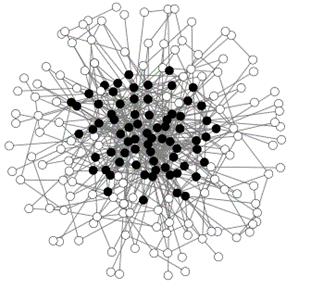
\includegraphics[width=0.25\columnwidth]{Fig303-CorePeriphery.png}
	 	\caption{Example network with core-periphery structure from Newman (2018).}\label{fig:303CorePeriphery}
	\end{figure}	
	
	The notion of a core-periphery network structure began with Borgatti \& Everett (2000), whose model assumes two classes of nodes: one highly inter-connected group with many connections to nodes in the other group (the core) and another made up of nodes that are only loosely connected to the earlier group (the periphery). This notion has been refined to allow for the partition of the nodes into three or more classes, and community detection algorithms have been developed to determine such partitions. However, in the case of our model, we will assume that our trade network follows the simpler model.
	
	A common algorithm to distinguish between core and peripheral nodes is the \textit{k-core algorithm}. A \textit{k-core} refers to a subgraph in the network where all nodes have at least $k$ neighboring vertices. The k-core algorithm involves progressively removing nodes with degrees less than $k$ from the graph until no such nodes are left, leaving us with the network's k-core. Nodes with degree 1, for example, form the 1-core, nodes with degree 2 form the 2-core and so on. \cite{borgatti2018analyzing}
	
	Another common algorithm is to assume that nodes in the core have a higher degree compared to those in the periphery. By setting a threshold degree, one can separate the core nodes from the peripheral nodes. Despite being simple, Newman (2018) argues that the results given by this algorithm do not differ very considerably from those yielded by more sophisticated community detection algorithms. 

	Hand-in-hand with a network exhibiting core-periphery structure is the inherent systemic risk. Primarily used in finance, \textit{systemic risk} is a term used to refer to the risk of collapse of any system due to events at the individual level. As Motter \& Lai (2002) point out, nodes which are highly connected and associated with greater loads are more susceptible to cascades which end up affecting (and ultimately upending) the entire network. Thus, networks with a  core-periphery structure are more susceptible to systemic risk.
	
	%-----------------------------
	% Section 3.3
	%-----------------------------
	\section{Shock Propagation in Trade Networks}
	\label{sec:33ShockPropagation}
	
	Burkholz \& Schweitzer (2019) provide a basic model for shock propagation, in the form of a one-time exogenous shock. They trigger a supply-side shock to some country $k$, which thereby creates a demand deficit $dd_k$ at $t = 1$. This results in country $k$ reducing its exports in $t = 2$, such that the reduction fully compensates for the demand deficit (i.e., $dd_k = 0$). Say country $i$ imports from country k. At $t = 2$, country $i$ will now have to face a demand deficit $dd_i$, which it will then try to reduce in the next time step. Thus, this one-time shock results in a cascade, which stops when no country with a demand deficit can further reduce its exports. They account for both equal shocks and proportional shocks (where the supply-side shock is proportional to country $k$’s GDP.
	
	Gephart et al. (2016) provide an even more detailed framework for shock propagation in the trade network. More formally, they begin with $n$ trading partners and an initial trade matrix $F^{0}$. The trade matrix is structured such that the trade flow from country $i$ to country $j$ at time $t$ is given by $F_{ij}^{t}$. The total exports at time $t$ to country $k$, denoted by $e_{k}^{t}$ is given by the row sums; i.e., 
	
	\begin{equation}
	\label{eqn:320exports} e_{k}^{t} = \sum_{l = 1}^{n} F_{kl}^{t}
	\end{equation}
	
	They then introduce a perturbation to the trade network by reducing the supply of some country $i$ at iteration $t = 1$. This creates a demand deficit for country $i$, which it compensates for by reducing its exports to its trading partners by a fraction $s$, where $0 < s \leq 1$ (the shock parameter). That is, for affected country $i$,
	
	\begin{equation}
	\label{eqn:321exportShock1} e_{i}^{1} = (1 - s) e_{i}^{0}
	\end{equation}
	
	while 
	
	\begin{equation}
	\label{eqn:322exportShock2} e_{i}^{1} = e_{j}^{0}
	\end{equation}
	
	for all countries $ j \neq i$. They also assume that the reduction in supply is not fully compensated for, and that only a proportion $q$, where $0 < q \leq 1$ (the spread parameter) is transmitted. 
	
	The shock to country $i$, given by $qse_i^{0}$, is transmitted to the export trading partners in accordance to the transfer matrix $T^{t}$. Tamea, et al. (2016) assumed that the received impulse is passed on proportionally with respect to the export volume, so that the elements of the transfer matrix at $t = 0$ are given by
	
	\begin{equation}
	\label{eqn:323transferMatrix1} T_{ij}^{0} = \frac{F_{ij}^{0}}{e_{i}^{0}}
	\end{equation}
	
	Gephart et al. (2016) modify this by incorporating willingness to pay. In their case, $T_ij$ is given by
	
	\begin{equation}
	\label{eqn:324transferMatrix2} T_{ij}^{0} = \frac{F_{ij}^{0}g_{j}^{\alpha}}{\sum_{j' = 1}^{n} F_{ij'}^{0}g_{j'}^{\alpha}}
	\end{equation}
	
	where $g_{j}$ is the per-capita GDP of country $j$, proxying for a region's willingness to pay and $\alpha \geq 0$ is the degree of influence of per-capita GDP on the distribution of the shock. When we increase $\alpha$, shocks are directed more towards regions with higher per-capita GDPs and less towards those with lower per-capita GDPs. This is because given the increase in prices due to decreased supply, high-income countries tend to be more willing to pay as opposed to low-income ones.
	
	They let the matrix E denote an export-only variant of the adjacency matrix for shocked nodes. That is, $E_{ij}= 1$  if a trade link exists from shocked country $i$ to country $j$ and 0 otherwise. Thus, at $t = 1$, the trade matrix $F^{1}$ is given by
	
	\begin{equation}
	\label{eqn:325dynamics1} F_{ij}^{1} = 
	\left[
	F_{ij}^{0} - T_{ij}^{0} * E_{ij} * qse_{i}^{0}
	\right]^{+}
	\end{equation}
	
	where $*$ denotes element-wise/scalar multiplication and the superscript plus sign is used to indicate the maximum of the value in the parentheses and zero. They update the export vector $e^{1}$ and transfer matrix $T^{1}$ accordingly, with respect to the new trade matrix $F^{1}$.
	 
	The starting node's export partners now have their imports reduced. This creates a demand deficit in these countries and in compensation, they reduce their own exports to their export partners. This then creates a demand deficit, so that these export partners reduce their exports to their export partners.
	
	This continues until a node is unable to pass the shock any further because its exports have been reduced to zero.
	
	Thus, the dynamics can be iteratively defined as follows:
	
	\begin{equation}
	\label{eqn:326dynamics2} F_{ij}^{t + 1} = 
	\left[
	F_{ij}^{t} - T_{ij}^{t} * E_{ij} * qse_{i}^{t}
	\right]^{+}
	\end{equation}
	
	In total, the model by Gephart et al. (2016) features three modifiable parameters: the degree of spread ($q$), the degree of shock ($s$) and the willingness-to-pay proxy ($\alpha$). The model is run for different parameters, and then the results are averaged across all runs.
	
	Intrinsic to the model above are a number of assumptions. These include:
	
	\begin{enumerate}
		\item The shocks are assumed to have occurred at the start of the following year.
		\item The shock takes into effect almost immediately. The time scale of the shock is independent of the shock's origin or recipient.
		\item There are global parameters (shock parameter, spread parameter) which define the extent and spread of the shock, regardless of the starting node.
		\item Demand for the good in all countries is assumed to be fixed. Moreover, countries are assumed to prioritize domestic demand over international and will thus try to keep fluctuations in domestic prices as small as possible. Thus, in response to decreased domestic supply, they reduce exports.
		\item The shocks are spread proportionally to a country's export partners.  
		\item The model terminates when one of the nodes fails – that is, if one of the nodes can no longer reduce its exports to compensate for the demand deficit.  
	\end{enumerate}
	
	Based on this model, we can also formulate an analogous agent-based model which simulates a one-time exogenous shock on a country’s imports, corresponding to a sudden increase in supply or the imposition of trade sanctions in the real world. The decrease in imports will propagate to the country’s import partners, resulting in supply surpluses for these countries. In response, these countries will reduce their imports to other countries, resulting again in supply surpluses for these countries’ import partners. The shock will continue to cascade until a country can no longer decrease its imports to compensate for the supply surplus. 
	Mathematically, this model will follow the dynamics outlined earlier. However, the total imports at time t to country k, denoted by $i_{k}^{t}$ is given by the column sums; i.e.,
	
	\begin{equation}
	\label{eqn:327imports} i_{k}^{t} = \sum_{l = 1}^{n} F_{lk}^{t}
	\end{equation}
	
	Furthermore, the perturbation to country i in this model is now given by
	
	\begin{equation}
	\label{eqn:328importShock} i_{i}^{1} = (1 - s) i_{i}^{0}
	\end{equation}
	
	The shock to country $i$, now given by $qsi_{i}^{0}$, is then transmitted to the import trading partners in accordance to the transfer matrix $T^{t}$. In line with Tamea et al. (2016),  we now define $T^{t}$ to have the elements 
	
	\begin{equation}
	\label{eqn:329transferMatrix} T_{ij}^{0} = \frac{F_{ji}^{0}}{i_{i}^{0}}
	\end{equation}
	
	We let the matrix $I$ denote an import-only variant of the adjacency matrix for shocked nodes. That is, $I_{ji}= 1$  if a trade link exists from country $j$ to shocked country $i$ and 0 otherwise. Thus, using the equations defined in equations (\ref{eqn:327imports}) to (\ref{eqn:329transferMatrix}), we define the dynamics of the demand-side model to be as follows:
	
	\begin{equation}
	\label{eqn:330dynamics} F_{ji}^{t + 1} = 
	\left[
	F_{ji}^{t} - T_{ji}^{t} * I_{ji} * qsi_{i}^{t}
	\right]^{+}
	\end{equation}
	
	where $*$ denotes element-wise/scalar multiplication and the superscript plus sign is used to indicate the maximum of the value in the parentheses and zero. Again, this continues until a node is unable to pass the shock any further because its imports have been reduced to zero. The process is repeated for all countries in the trade network. The same assumptions and simulation metrics apply to the demand-side model, which include:
	
	\begin{enumerate}
		\item The shocks are assumed to have occurred at the start of the following year.
		\item The shock takes into effect almost immediately. The time scale of the shock is independent of the shock's origin or recipient.
		\item There are global parameters (shock parameter, spread parameter) which define the extent and spread of the shock, regardless of the starting node.
		\item Demand for the good in all countries is assumed to be fixed. Moreover, countries are assumed to prioritize domestic demand over international and will thus try to keep fluctuations in domestic prices as small as possible. Thus, in response to increased domestic supply, they reduce imports.
		\item The shocks are spread proportionally to a country's import partners.  
		\item The model terminates when one of the nodes fails – that is, if one of the nodes can no longer reduce its imports to compensate for the supply surplus.  
	\end{enumerate}
	
	In general, the first agent-based simulation (supply-side decrease) represents the network of outgoing links, while the second agent-based simulation (supply-side increase) represents the network of incoming links. Thus, any conclusions we draw from both simulations will apply to the networks that correspond to them.
	
	To assess the cascade, Loser \& Segel (n.d.) used the \textit{cascade size}, which is number of edges affected by the cascade, and the \textit{cascade depth}, which is the number of iterations the cascade takes before the simulation terminates.
	
	Gephart et al. (2016) grouped all the countries in the trade network into 18 regions and use those as the nodes in the network. To determine the effects of the cascade, they calculated the \textit{exposure} of the region, which is the percent of initial shock absorbed in a particular region. This determines how vulnerable other regions are to perturbations in certain regions.

\chapter{Methodology}
\label{chap:4Methodology}

This chapter contains the actual methods used to conduct the study. The data was first pre-processed to enable the construction of the world trade network. The resulting networks were then characterized based on the measures outlined in Chapter 3 to aid in our understanding of the results when we implement shock propagation in the network afterwards. 

	\section{Data Pre-processing}
	\label{sec:41dataPreprocessing}
	
	As discussed before, the study will simply focus on the integrated circuit trade network. Trade data for this particular good during the years 2013-2017 was collected from the UN Comtrade database using the tradedownloader tool (linked here: \underline{https://github.com/ejokeeffe/tradedownloader}). We cleaned the data using the Pandas package in Python to make it amenable to the construction of a trade network. 
	
	The data itself is subject to several issues. For one, it is given from the perspective of the reporting country, meaning that there will be bilateral asymmetries between the export and import data. If the reporting country has a devalued currency (e.g., China), the exports may appear to be larger than they really are. The data is also reported in nominal US\$, which makes it difficult to make year-on-year comparisons due to the effects of inflation. 
	
	Lastly, the bilateral nature of the data will result in persistent feedback loops when we simulate economic shocks on the network. As an example, suppose we begin with a supply-side decrease on China. This will go on to affect the Philippines, one of its export partners, and in response, it propagates the shock to all its export partners, which includes China. In effect, the two countries will continue to “shock” each other until the simulation terminates.
	To address the first issue, Reyes, Fagiolo \& Schiavo (2010) simply averaged the export and import data between any two countries to get a rough estimate for the trade flow. The second issue can easily be addressed by setting the earliest year as the base year and deflating the figures in succeeding years based on reported US Consumer Price Index (CPI) from the World Bank. We can address the third issue and remove most of the feedback loops in the network by creating a unilateral network where the weights will be the net exports from the source country to the target country.
	
	\section{Network Visualization and Characterization}
	\label{sec:42networkVisualizationCharacterization}
	
	After cleaning the data, we then constructed the unilateral networks using the NetworkX package in Python. They were then visualized using NetworkX, employing a force-based algorithm to keeps well-connected nodes closer to each other.
	Using the functions in the NetworkX package, we then characterized the resulting network. As discussed in Chapter 3, we computed the network density, total link weight and degree assortativity of the network over time to get a picture of how the trade network has evolved through the years. To determine which nodes are relatively more important, we used the centrality measures discussed in Chapter 3 and compared them with each other to detect any notable patterns.
	
	\section{Shock Propagation}
	\label{sec:43shockPropagation}

	Based on the basic model suggested by Burkholz \& Schweitzer (2019) and Gephart et al. (2016) outlined in Chapter 3, we implemented an agent-based model on the constructed networks by simulating a one-time exogenous shock on a country’s exports and imports. In the real world, the former can represent a sudden decrease in supply potentially due to the imposition of trade sanctions while the latter can correspond to a sudden increase in supply. 
	
	\begin{figure}[!h]
		\centering
		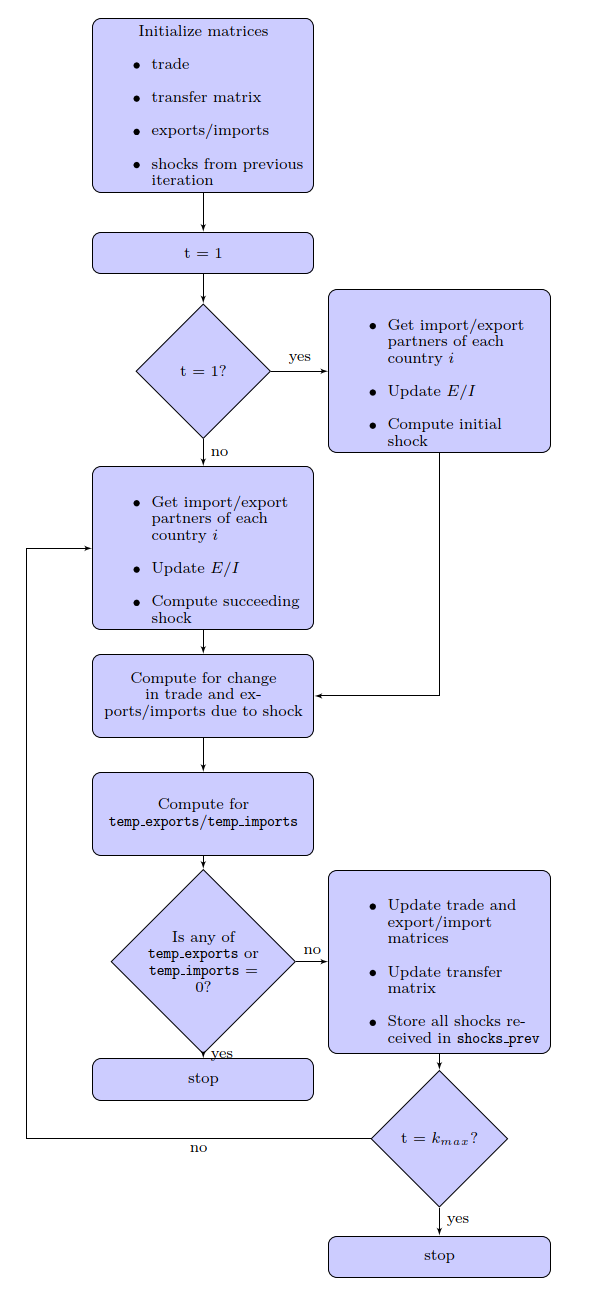
\includegraphics[scale = 0.7]{Fig401-Flowchart.png}
		\caption{Flowchart summarizing the shock propagation algorithm for the IC trade network.}\label{fig:401Flowchart}
	\end{figure}
	
	The algorithm is summarized in Figure \ref{fig:401Flowchart}. The models were built based on trade networks which themselves are based on annual data regarding integrated circuit trade given by the United Nations' Comtrade database. In particular, we used their latest dataset from 2017. We set $k_{max}$, the maximum number of possible iterations, to 50. 
	
	After performing the agent-based simulation, we examined the impact of the cascade on the network using three metrics: cascade size, cascade depth and exposure. The \textit{cascade size } denotes the number of unique affected nodes in the cascade. The \textit{cascade depth} refers to the number of iterations it takes for the shock to cascade through the network until the simulation terminates. \cite{losercs224w} As explained earlier, we define the terminating condition to be one where a shocked country can no longer reduce its exports or imports to compensate for the demand deficit or supply surplus resulting from being shocked, respectively. The \textit{exposure} refers to the amount of a shock that a country receives in the simulation relative to the initial shock. \cite{gephart2016vulnerability} We used these metrics to identify any underlying core-periphery structure, to determine which countries are the most vulnerable to shocks to the Philippines and to determine which countries the Philippines is the most vulnerable to when shocked. Following Gephart et al. (2016), we averaged the results across different values of the parameters, considering values from 0 to 1 in increments of 0.1 for the shock and spread parameters. This assumes that these different scenarios are equally likely. 
	
	We then use the degree threshold method identified in Newman (2018) to identify core and peripheral nodes in the network. As we will see later on, however, the degree is not informative enough in a network as a measure of importance, especially in the context of identifying which nodes carry more systemic risk.
	
	Using the cascading failure model from Motter \& Lai (2002), Li et al. (2014) formulated a centrality measure for industries in the world input-output network in the context of an industry's impact on the rest of the network as a result of an economic shock to it. In their work, shocks are propagated to each node and a critical threshold value is computed for each industry. They then use this to rank the economic importance of each industry in the world input-output network. 
	
	We combine the degree threshold method with the aforementioned approach to calculate a minimum shock threshold for each country in the integrated circuit trade network. This minimum shock threshold represents the minimum amount of shock needed for a country to be considered a core node, setting the spread parameter to 1 (i.e., all of the shocks are transmitted). The definition of a core node is heuristic and will primarily rest on the results obtained from the cascade size and cascade depth. The calculations will be done using a modified bisection search algorithm.
	
	Using the rank-size distribution of the computed minimum shocks, we then 
	use threshold shock values (which are also heuristic) to determine which nodes constitute which group.
	
\chapter{Results and Discussion}
\label{chap:5Results}
This chapter will present the results based on the procedures outlined in Chapter 4. Sections 5.1 and 5.2 discuss the characteristics of the networks resulting from the trade data we obtained. In Sections 5.3 and 5.4, we examine the results of the supply-side agent-based simulations performed on the networks.

	\section{Network Visualization}
	\label{sec:51networkVisualization}
	
	\begin{figure}[!h]
		\centering
		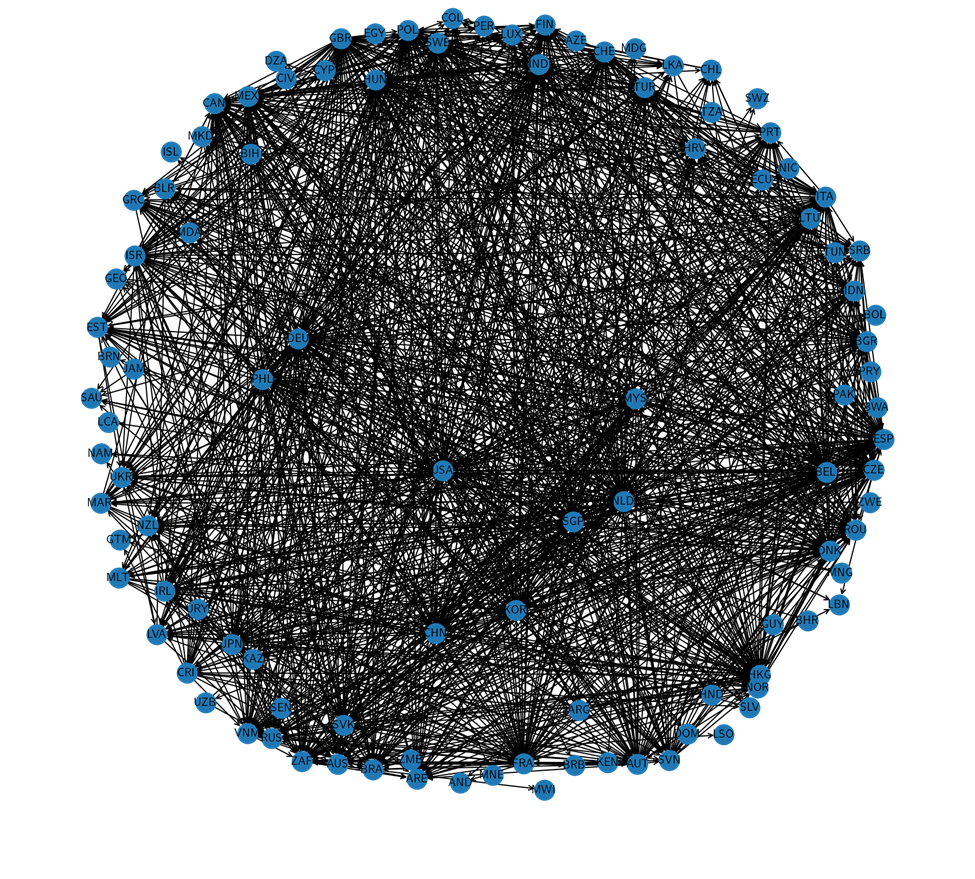
\includegraphics[width=0.5\columnwidth]{Fig501-ICNetwork.png}
		\caption{2017 integrated circuit network using a force-directed layout.}\label{fig:501ICNetwork}
	\end{figure}
	
	Figure \ref{fig:501ICNetwork} shows the 2017 integrated circuit network. It was constructed using the NetworkX package in Python with a force-directed layout, so as to keep well-connected nodes close to each other. Note the similarity between Figure \ref{fig:501ICNetwork} and Figure \ref{fig:303CorePeriphery} in Chapter 3, suggesting that the network may possibly have an underlying core-periphery structure.
	
	\section{Network Characterization}
	\label{sec:52networkCharacterization}
	
		\subsection{Network-Level Measures}
		\label{ssec:521networkLevel}
		
		The trade networks from Section 5.1 were constructed for years 2013-2017 and for each one, we computed the link density, total link weight and degree assortativity to do year-on-year comparisons. 
		
		The link density, for example, quantifies how well-connected the nodes in a network are (or how complete the graph is, using graph-theoretic terminology). Coupled with this, we can also look at the total link weight per year, as in Burkholz \& Schweitzer (2019). The link density tells us how many links there are in the network at any point in time while the total link weight per year tells us the trade volume that goes on in the network at any point in time.
		
		\begin{figure}[!h]
			\centering
			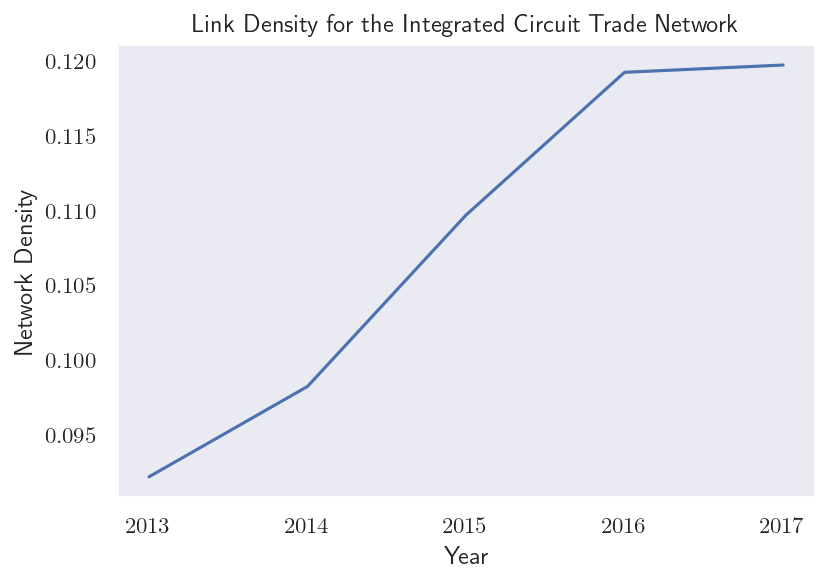
\includegraphics[width=0.5\textwidth]{Fig502-LinkDensity.png}
			\caption{Link density for the integrated circuit trade network.}\label{fig:502LinkDensity}
		\end{figure}
	
		\begin{figure}[!h]
			\centering
			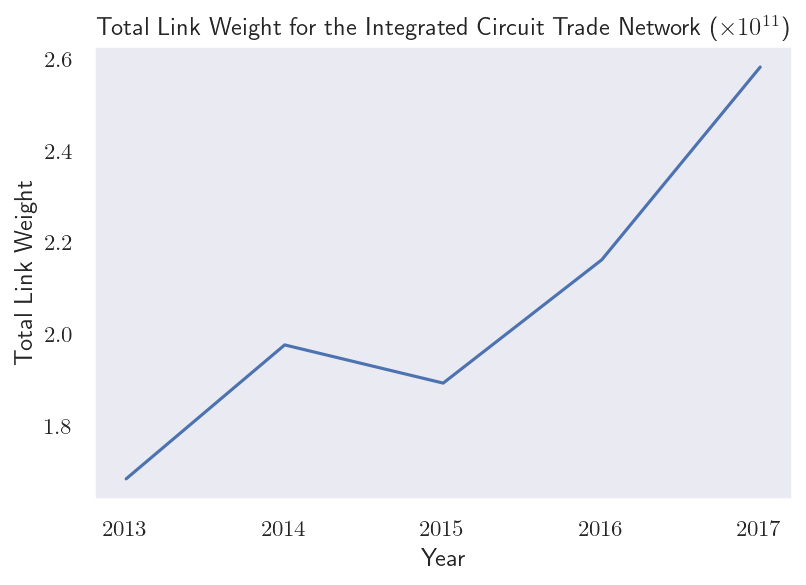
\includegraphics[width=0.5\textwidth]{Fig503-TotalLinkWeight.png}
			\caption{Total link weight for the integrated circuit trade network.}\label{fig:503TotalLinkWeight}
		\end{figure}
			
		Figures \ref{fig:502LinkDensity} and \ref{fig:503TotalLinkWeight} show that both the density of the trade network and the total link weight have had a generally increasing trend throughout the years. Countries have been trading more frequently and in larger quantities with each other in the integrated circuit network, presumably as a result of globalization.
		
		The assortativity coefficient refers to the Pearson correlation of the degrees of two linked nodes. A positive value indicates a correlation between nodes of the same degree whereas a negative value indicates a correlation between nodes of different degrees. That is, a positive value signifies that nodes of similar degrees tend to associate with each other while a negative value signifies that high-degree nodes and low-degree nodes tend to associate with each other. As such, we expect to see low values for the assortativity coefficient as there does not seem to be any preferential attachment among high-degree or low-degree nodes in the network.
		
		Assortativity has also been used to indicate whether or not a network has a core-periphery structure. A core-periphery structure is one characterized by a core of high-degree nodes surrounded by a periphery of lower-degree nodes. Assortative networks (i.e., networks for which the assortativity coefficient is positive) are said to be indicative of this type of structure. Given what we have observed in the graphs, we expect to observe an assortative structure in the input-output network.
		
		\begin{figure}[!h]
			\centering
			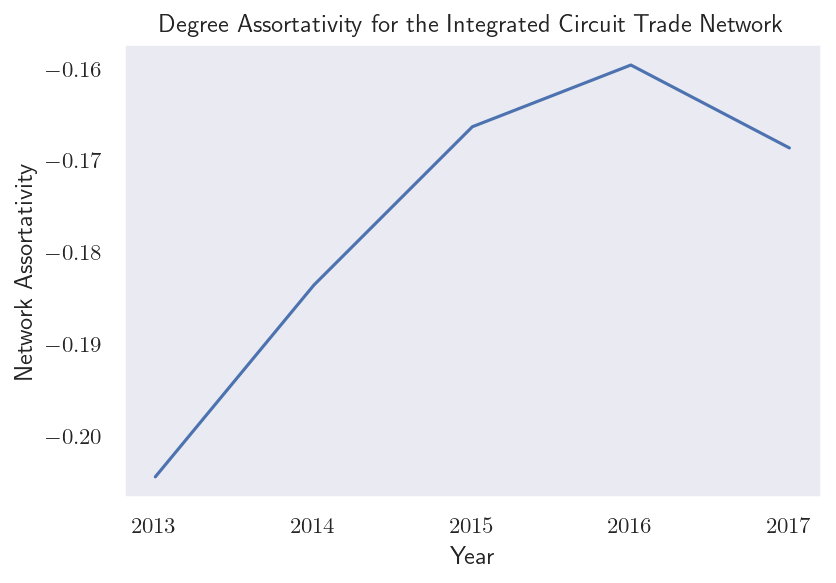
\includegraphics[width=0.5\textwidth]{Fig504-Assortativity.png}
			\caption{Degree assortativity for the integrated circuit trade network.}\label{fig:504Assortativity}
		\end{figure}
	
		Figure \ref{fig:504Assortativity} reveals that the assortativity values for the integrated circuit trade network are slightly negative, suggesting that the network is quite disassortative. This means that high-degree/low-degree countries in the network do not exhibit preferential attachment and prefer to trade with each other. This could also mean that the relatively poorly connected countries predominantly use highly-connected countries as trade hubs to access the rest of the network (Fagiolo, Reyes \& Schiavo, 2008). 
		
		The assortativity coefficient has been increasing over the years, however, which can potentially be attributed to high-degree countries forming more links with each other – again, a possible by-product of globalization. 
		
		Overall, all network-level measures seem to be increasing year on year, due primarily to globalization. Note however that there does not seem to be a drastic change in the values from year to year.
		
		\subsection{Centrality Measures}
		\label{ssec:522centrality}
		
			Centrality measures have been calculated for years 2013-17. 
			However, the observations made here have been similar to those made for previous years. As such, for the sake of brevity, we only present the results for the 2017 network in this section.
	
			\subsubsection{Degree Centrality}
			\label{ssec:5221degree}
			
			We first check the in-degree and out-degree of each node. The degree is the number of edges adjacent to the node. In particular, the in-degree refers to the number of edges pointing towards the node while the out-degree refers to the number of edges pointing away from the node.
			
			\begin{figure}[!h]
				\centering
				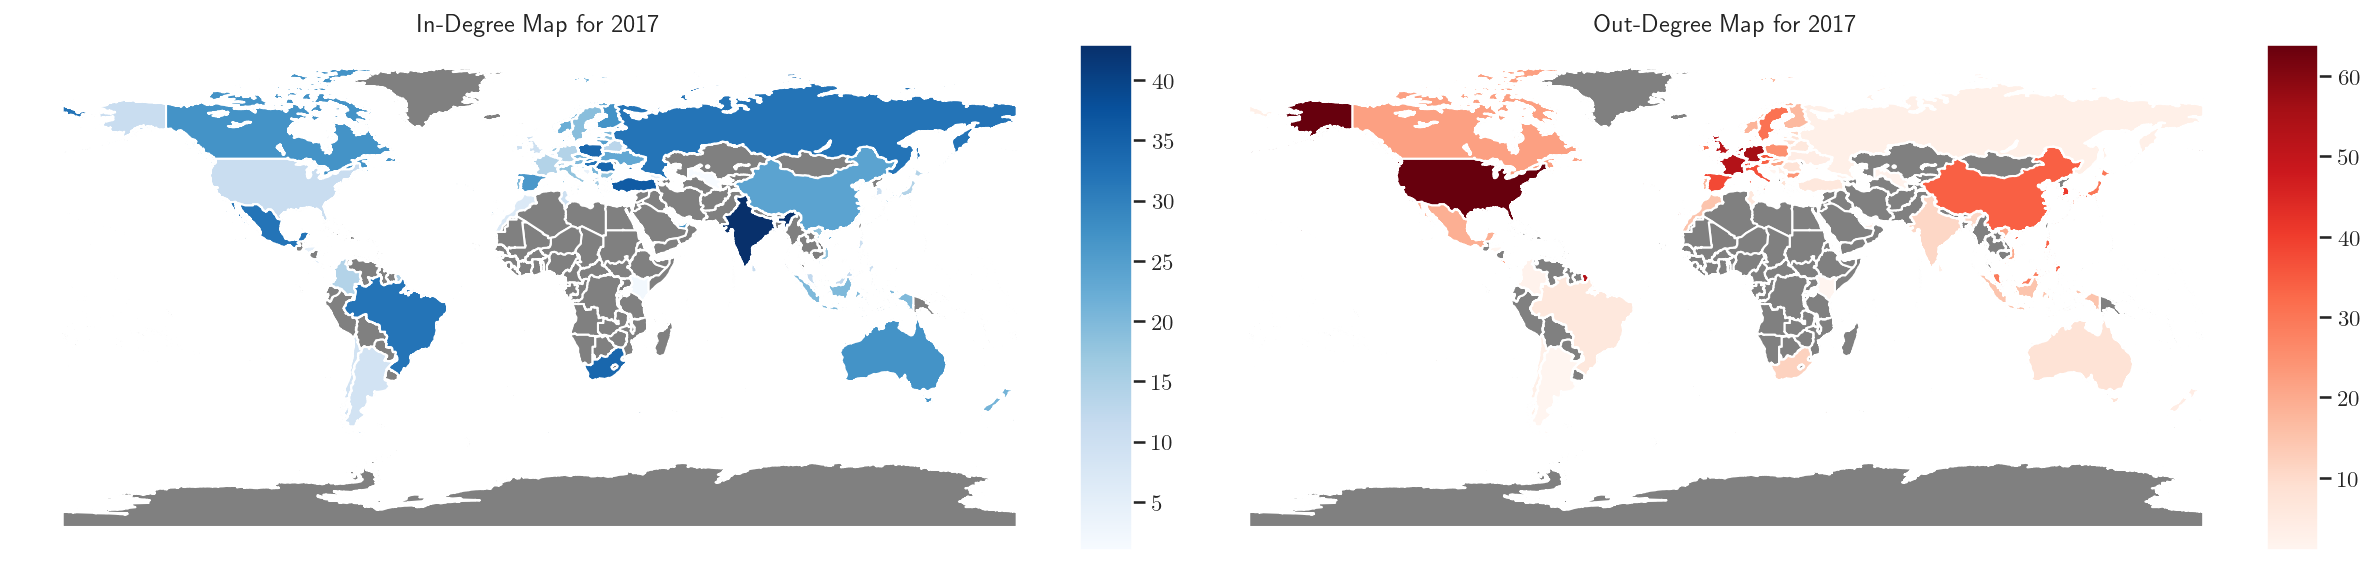
\includegraphics[width=\textwidth]{Fig505-DegreeMap.png}
				\caption{In-degree and out-degree maps for the 2017 integrated circuit trade network.}\label{fig:505DegreeMap}
			\end{figure}
			
			Figure \ref{fig:505DegreeMap} shows the in-degree and out-degree maps for the 2017 integrated circuit trade network. The maps show that countries like India, Brazil, Spain, Turkey, Romania, Mexico, South Africa and Russia have high in-degrees. On the other hand, countries like the US, France, Germany, the UK and South Korea have high out-degrees.
			
			Note that most of the countries in the East and Southeast Asian, Western European and North American regions seem to exhibit moderate to high in-degrees and out-degrees, potentially denoting the regions' midstreamness in the integrated circuit value chain overall. The Philippines, in particular, has consistently had a higher out-degree than in-degree, which makes 
			sense as integrated circuits are one of its primary exports.
			
			\begin{figure}[!h]
				\centering
				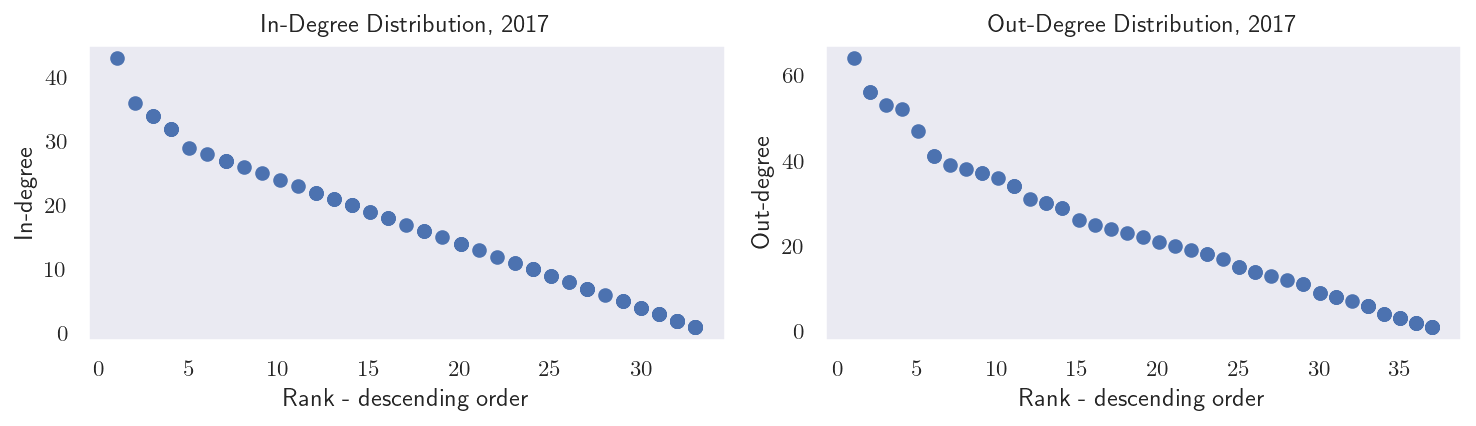
\includegraphics[width=\textwidth]{Fig506-DegreeDistribution.png}
				\caption{In-degree and out-degree distributions for the 2017 integrated circuit trade network.}\label{fig:506DegreeDistribution}
			\end{figure}
			
			Note from Figure \ref{fig:506DegreeDistribution} that both the in-degree and out-degree vary linearly with the rank. There are no apparent outliers in the network in terms of degree.
			
			\begin{longtable}{|l|l|r|l|l|r|}
				\caption{Top countries in terms of in-degree and out-degree for the 2017 integrated circuit trade network. \label{tab:tab01TopDegree}} \\
				\hline
				\textbf{\small Rank} & \textbf{\small Country} & \textbf{\small In-degree} & \textbf{\small Rank} &
				\textbf{\small Country} & \textbf{\small Out-degree} \\ 
				\hline
				\endfirsthead
				\hline
				\textbf{\small Rank} & \textbf{\small Country} & \textbf{\small In-degree} & \textbf{\small Rank} &
				\textbf{\small Country} & \textbf{\small Out-degree} \\ 
				\hline
				\endhead
				\hline
				\endfoot
				1 & India & 43 & 1 & USA & 64 \\
				2 & Turkey & 36 & 2 & Germany & 56 \\
				3 & Romania & 34 & 3 & The Netherlands & 56 \\
				4 & South Africa & 34 & 4 & France & 53 \\
				5 & Poland & 34 & 5 & UK & 52 \\
				6 & Brazil & 32 & 6 & Belgium & 47 \\
				7 & Hungary & 32 & 7 & Singapore & 41 \\
				8 & Russia & 32 & 8 & South Korea & 41 \\
				9 & Mexico & 32 & 9 & Israel & 39 \\
				10 & Slovakia & 29 & 10 & Spain & 38 \\
			\end{longtable}
		
			Lastly, Table \ref{tab:tab01TopDegree} shows that India has the highest in-degree, signifying that it has the highest number of import partners in 2017. Meanwhile, the US has the highest out-degree, signifying that it has the highest number of export partners. 
			
			\subsubsection{Strength Centrality}
			\label{ssec:5222strength}
			
			The degree centrality quantifies how central a node is in terms of the number of nodes it shares an edge with. This can be decomposed further into in-degree centrality (based on the number of nodes connected to it) and out-degree centrality (based on the number of nodes a node connects to). We can weight each connection by the edge weight, however, resulting in the in-strength and out-strength centrality measures.
			
			\begin{figure}[!h]
				\centering
				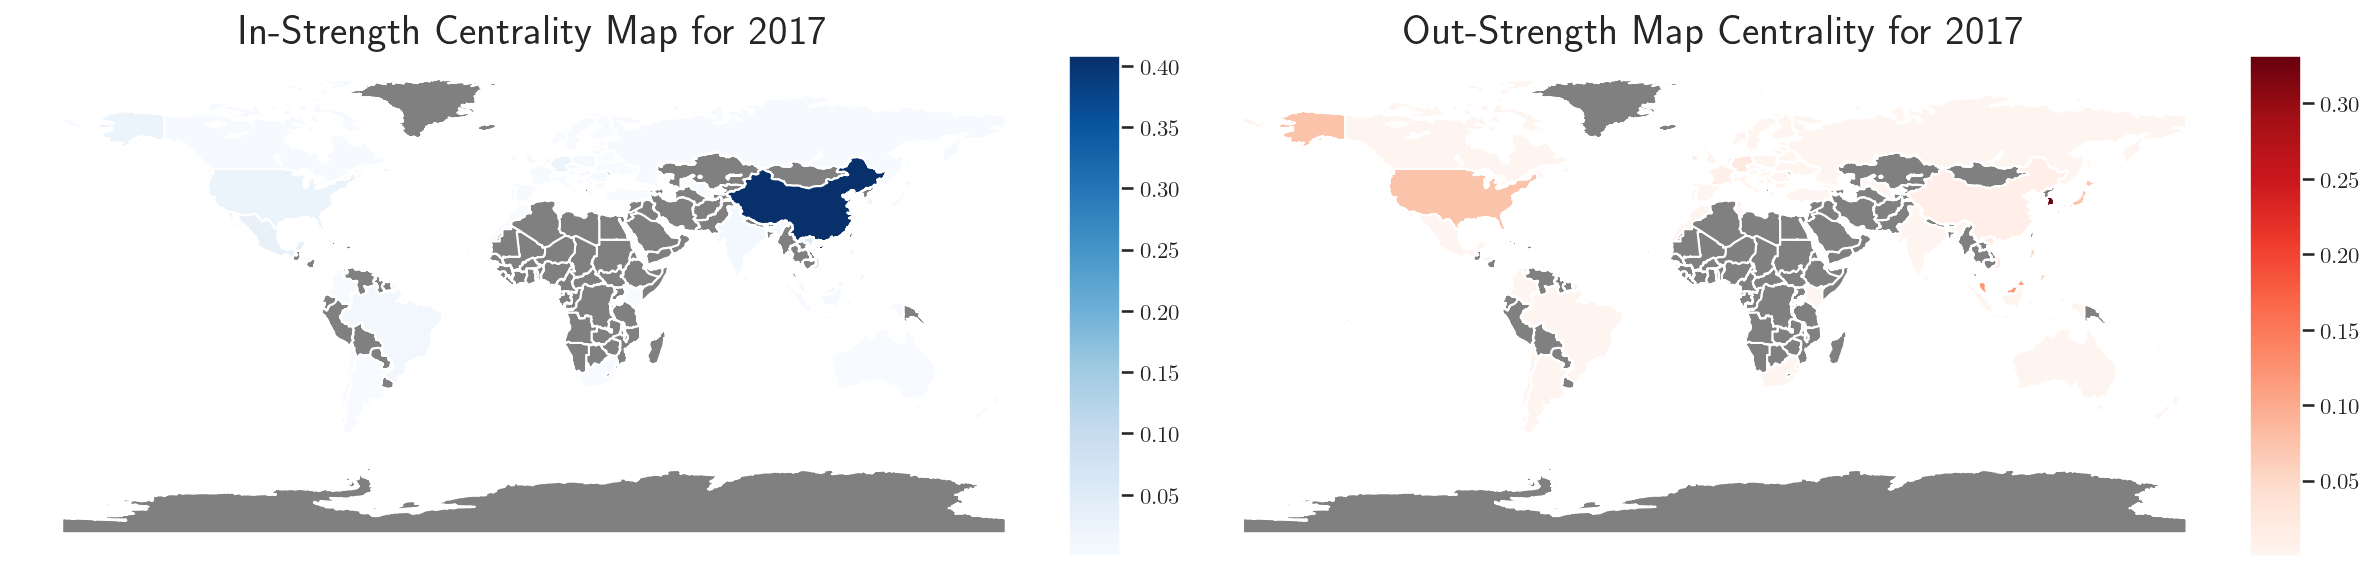
\includegraphics[width=\textwidth]{Fig507-StrengthMap.png}
				\caption{In-strength and out-strength centrality maps for the 2017 integrated circuit trade network.}\label{fig:507StrengthMap}
			\end{figure}
			
			The strength centrality differs from degree centrality in that it takes the weight of the links into account. Having done so, we can see that while China has not had the most export partners in any year, it is absolutely dominant in terms of in-strength centrality for all five years considered.
			
			China also ranks much higher in terms of in-strength centrality as opposed to out-strength centrality. Meanwhile, in terms of degree centrality (both in-degree and out-degree), it has consistently ranked mid-table. This means that it has China has a number of IC import partners with which it has a very large trade volume.  
			
			On the other hand, South Korea has consistently ranked first in the IC network in terms of out-strength centrality, this despite the fact that South Korea has never had the most import partners in any year. Again, this may be because it has a number of IC export partners with which it has a very large trade volume. Aside from South Korea, there are also a number of countries which can be regarded as important outgoing trade hubs in the IC trade network such as the US, Malaysia, Singapore, the Philippines and Japan.
		
			\begin{figure}[!h]
				\centering
				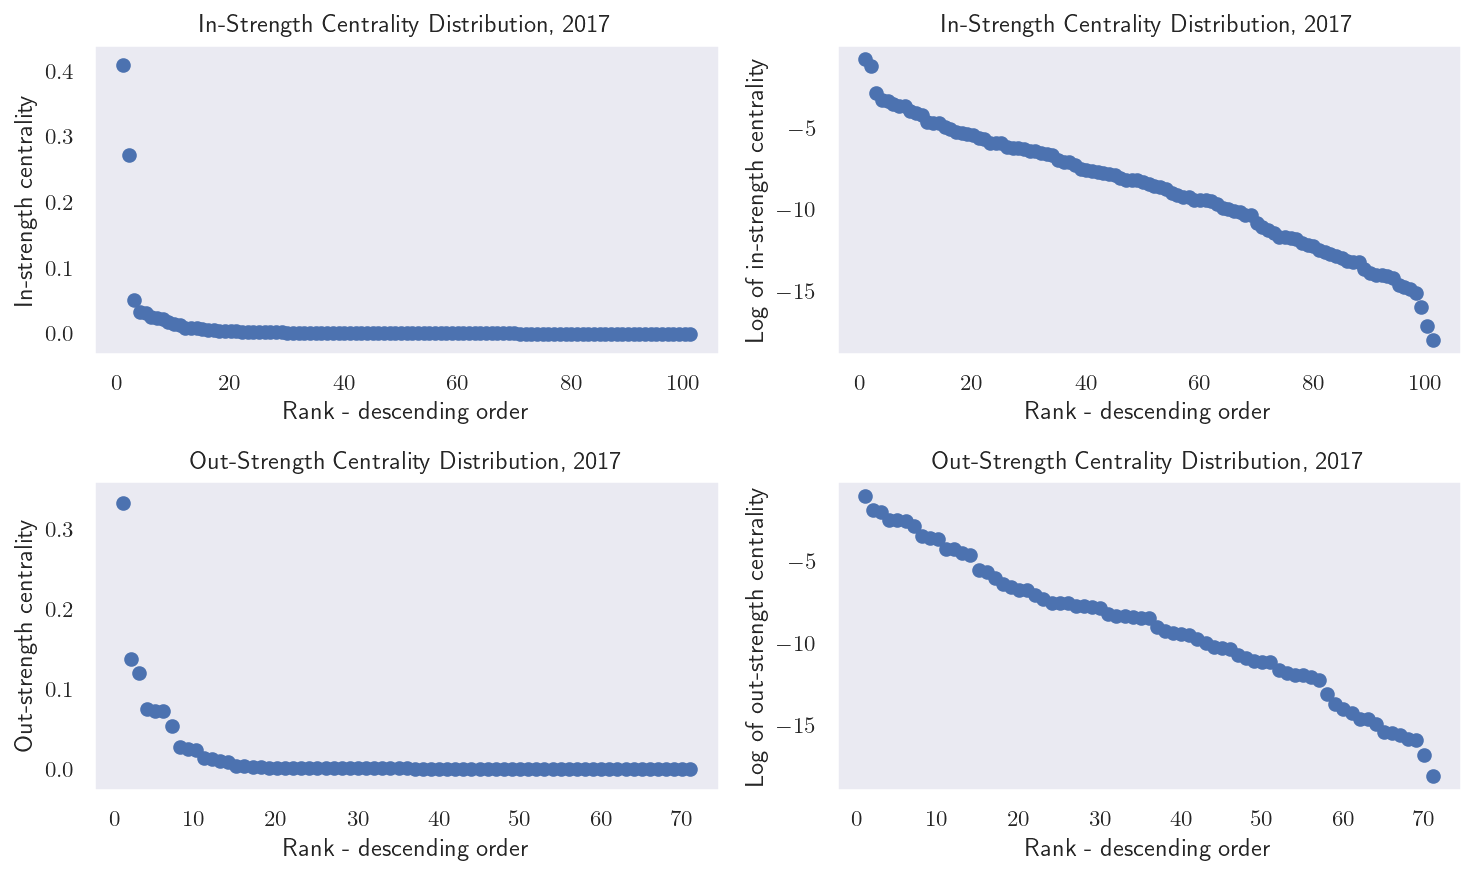
\includegraphics[width=\textwidth]{Fig508-StrengthDistribution.png}
				\caption{In-strength and out-strength centrality distributions for the 2017 integrated circuit trade network (linear and semilog).}\label{fig:508StrengthDistribution}
			\end{figure}
			
			Based on Figure \ref{fig:508StrengthDistribution}, from the linear plots, we see that there are very obvious outliers when we consider the link weights in the computation of the centrality. This stands in contrast with the distribution of the degree centrality, which is roughly uniform in spread. This signifies that the distribution is very heavily right-skewed, suggesting the presence of only a few incoming and outgoing hubs in the trade network which export/import a considerable amount of ICs (potentially forming the core of the network). The semilog plots, on the other hand, are roughly linear, suggesting that the rank is related to the in-strength and out-strength through an exponential function.
			
			\begin{longtable}{|l|l|r|l|l|r|}
				\caption{Top countries in terms of in-strength and out-strength centrality for the 2017 integrated circuit trade network. \label{tab:tab02TopStrength}} \\
				\hline
				\textbf{\small Rank} & \textbf{\small Country} & \textbf{\small In-strength} & \textbf{\small Rank} &
				\textbf{\small Country} & \textbf{\small Out-strength} \\ 
				\hline
				\endfirsthead
				\hline
				\textbf{\small Rank} & \textbf{\small Country} & \textbf{\small In-strength} & \textbf{\small Rank} &
				\textbf{\small Country} & \textbf{\small Out-strength} \\ 
				\hline
				\endhead
				\hline
				\endfoot
				1 & China & 0.4084433901 & 1 & South Korea & 0.3318328315 \\
				2 & Hong Kong & 0.2712190336 & 2 & Singapore & 0.1375397362 \\
				3 & Vietnam & 0.0504830260 & 3 & Malaysia & 0.1201234095 \\
				4 & Singapore & 0.0323640950 & 4 & USA & 0.0743141925 \\
				5 & Mexico & 0.0314456528 & 5 & Japan & 0.0724459271 \\
				6 & USA & 0.0251035442 & 6 & Hong Kong & 0.0722158284 \\
				7 & Germany & 0.0234046785 & 7 & Philippines & 0.0528225342 \\
				8 & The Netherlands & 0.0225012189 & 8 & Ireland & 0.0274227280 \\
				9 & Philippines & 0.0172273035 & 9 & Germany & 0.0244284761 \\
				10 & South Korea & 0.0148916951 & 10 & Vietnam & 0.0229935593 \\
			\end{longtable}
			
			We see that for the most part, China has the highest in-strength centrality, while South Korea has the highest out-strength centrality, signifying that they have the largest import and export IC market shares, respectively. For 2017, the centrality figures for China and South Korea suggest that on average, the former has a 40.84\% market share over total imports while the latter has a 33.18\% market share over total exports.
			
			The Philippines seems to have around the same figures throughout the years for both in-strength and out-strength centrality, possibly suggesting that it mostly imports raw materials/intermediate inputs and exports intermediate inputs/final products. In general, the presence of many East Asian/Southeast Asian countries in the top 10 suggests the regions' importance as trade hubs in the IC trade network.
			
			\subsubsection{Betweenness Centrality}
			\label{ssec:5223betweenness}
			
			The betweenness centrality is based on shortest paths, or geodesics. It quantifies how many of the geodesics between any two nodes in a network pass through a given node. Essentially, the betweenness centrality calculates how “in-between” each node is. For trade networks, it is calculated based on Equations (\ref{eqn:315weightTrade}) and (\ref{eqn:316shortestPathTrade}).
			
			\begin{figure}[!h]
				\centering
				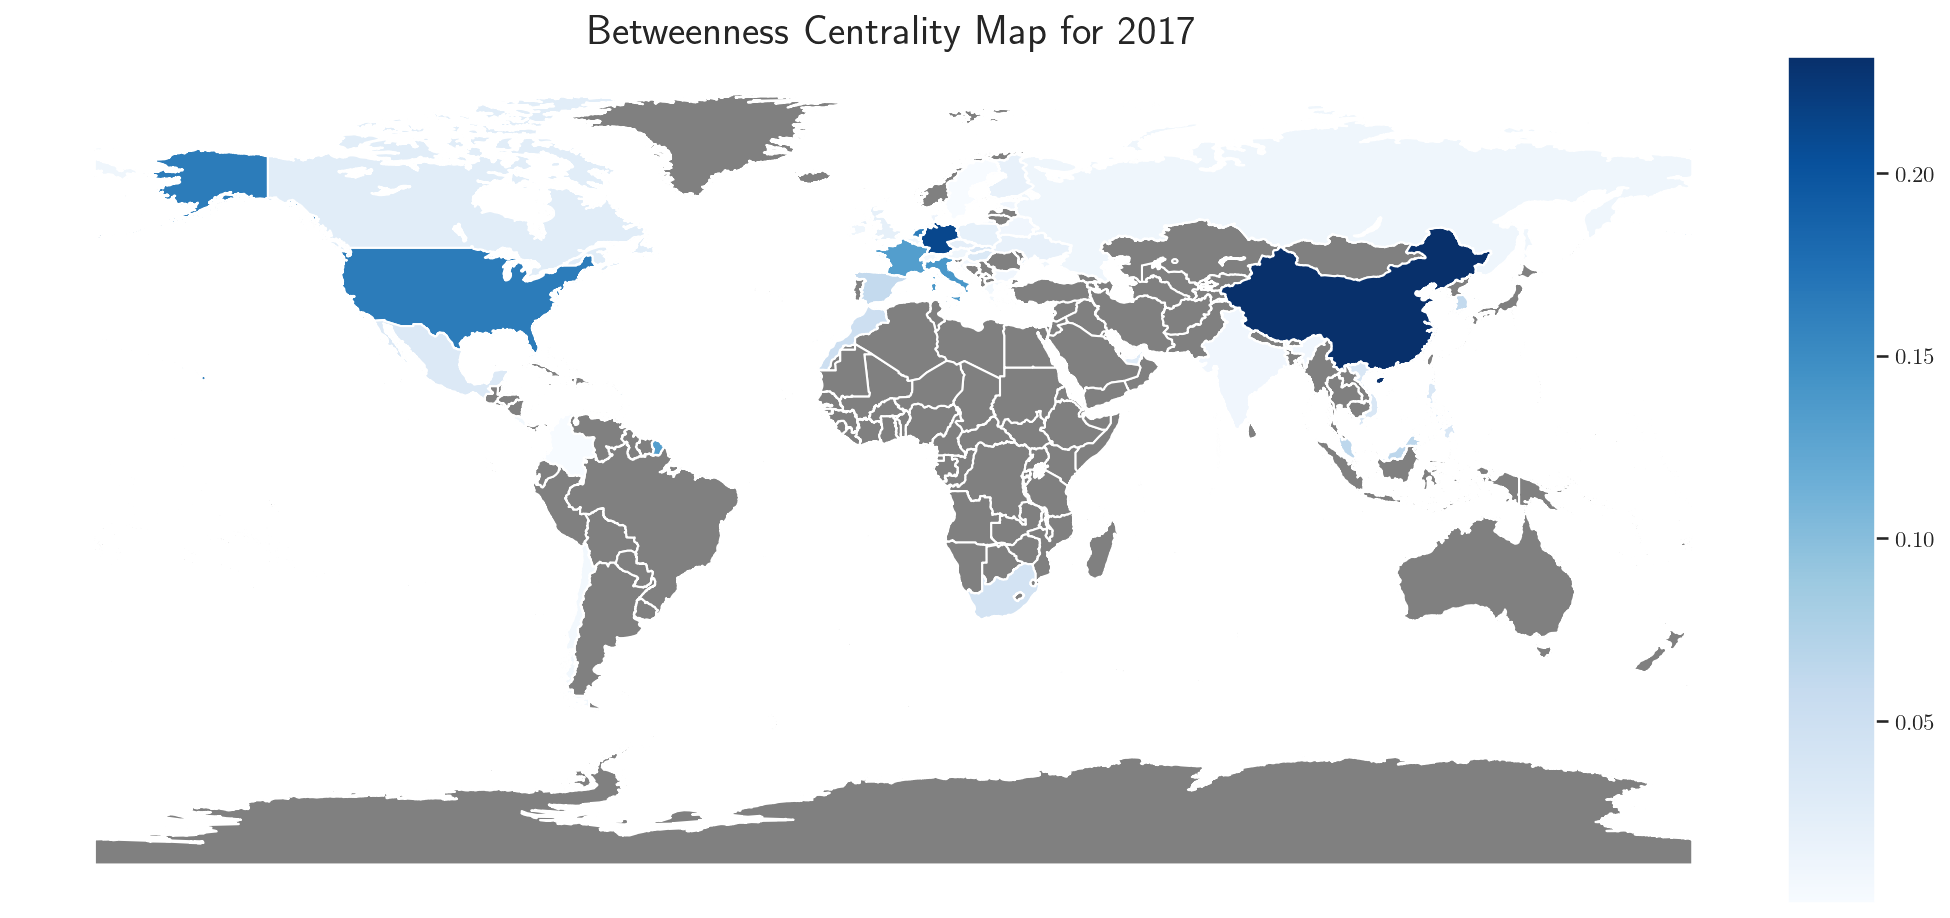
\includegraphics[width=\textwidth]{Fig509-BetweennessMap.png}
				\caption{Betweenness centrality map for the 2017 integrated circuit trade network.}\label{fig:509BetweennessMap}
			\end{figure}
			
			Figure \ref{fig:509BetweennessMap} shows that the usual suspects have the highest weighted betweenness centrality in the IC network: Germany, France, China, Vietnam, Singapore, Malaysia and the US. This means that these countries have a significant midstream presence in the IC value chain.
			
			\begin{figure}[!h]
				\centering
				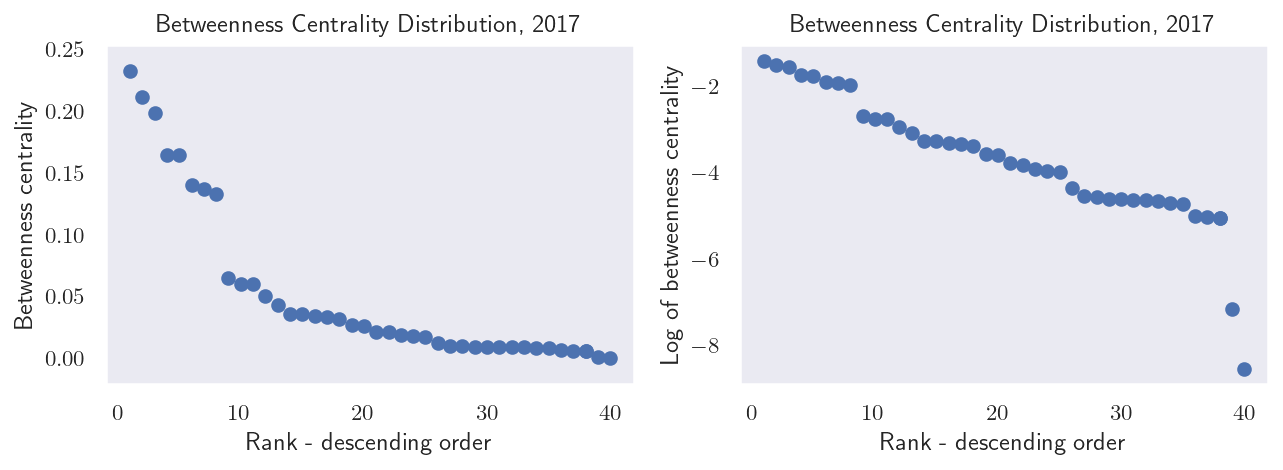
\includegraphics[width=\textwidth]{Fig510-BetweennessDistribution.png}
				\caption{Betweenness centrality distributions for the 2017 integrated circuit trade network (linear and semilog).}\label{fig:510BetweennessDistribution}
			\end{figure}
			
			From the distribution of the betweenness centrality, one can determine the presence of outlying nodes. As with before, this suggests the presence of trade hubs in the network – some of which are probably taking in or receiving a large amount of trade. As with before, the semilog plots are roughly linear in shape, meaning that the rank and the betweenness centrality are related through an exponential function.
			
			\begin{longtable}{|l|l|r|l|l|r|}
				\caption{Top countries in terms of betweenness centrality for the 2017 integrated circuit trade network. \label{tab:tab03TopBetweenness}} \\
				\hline
				\textbf{\small Rank} & \textbf{\small Country} & \textbf{\small Betweenness} & \textbf{\small Rank} &
				\textbf{\small Country} & \textbf{\small Betweenness} \\ 
				\hline
				\endfirsthead
				\hline
				\textbf{\small Rank} & \textbf{\small Country} & \textbf{\small Betweenness} & \textbf{\small Rank} &
				\textbf{\small Country} & \textbf{\small Betweenness} \\ 
				\hline
				\endhead
				\hline
				\endfoot
				1 & China & 0.2321695295 & 6 & Italy & 0.1397498133 \\
				2 & Germany & 0.2115384615 & 7 & Hong Kong & 0.1365758028 \\
				3 & Singapore & 0.1979088872 & 8 & France & 0.1331217326 \\
				4 & USA & 0.1646751307 & 9 & Malaysia & 0.0646938013 \\
				5 & The Netherlands & 0.1641150112 & 10 & South Korea & 0.0601194922 \\
			\end{longtable}
			
			From Table \ref{tab:tab03TopBetweenness}, China is the most in-between country in the IC trade network in terms of betweenness centrality, with 23.22\% of all inter-country geodesics passing through it at some point, after accounting for trade volume. This means that most high-value IC trade links are more likely to pass through China than through every other country.
			The list also contains the other countries we had identified earlier, including some countries in the East Asian/Southeast Asian region and the Western European region.
			
			\subsubsection{Eigenvector Centrality}
			\label{ssec:5224eigenvector}
			
			As opposed to the other three centrality measures, eigenvector centrality is often used as a measure of influence/prestige. Eigenvector centrality accounts for a node's neighbors and how well-connected they are. Thus, the higher the eigenvector centrality of a node, the more well-connected its neighbors are.
			
			\begin{figure}[!h]
				\centering
				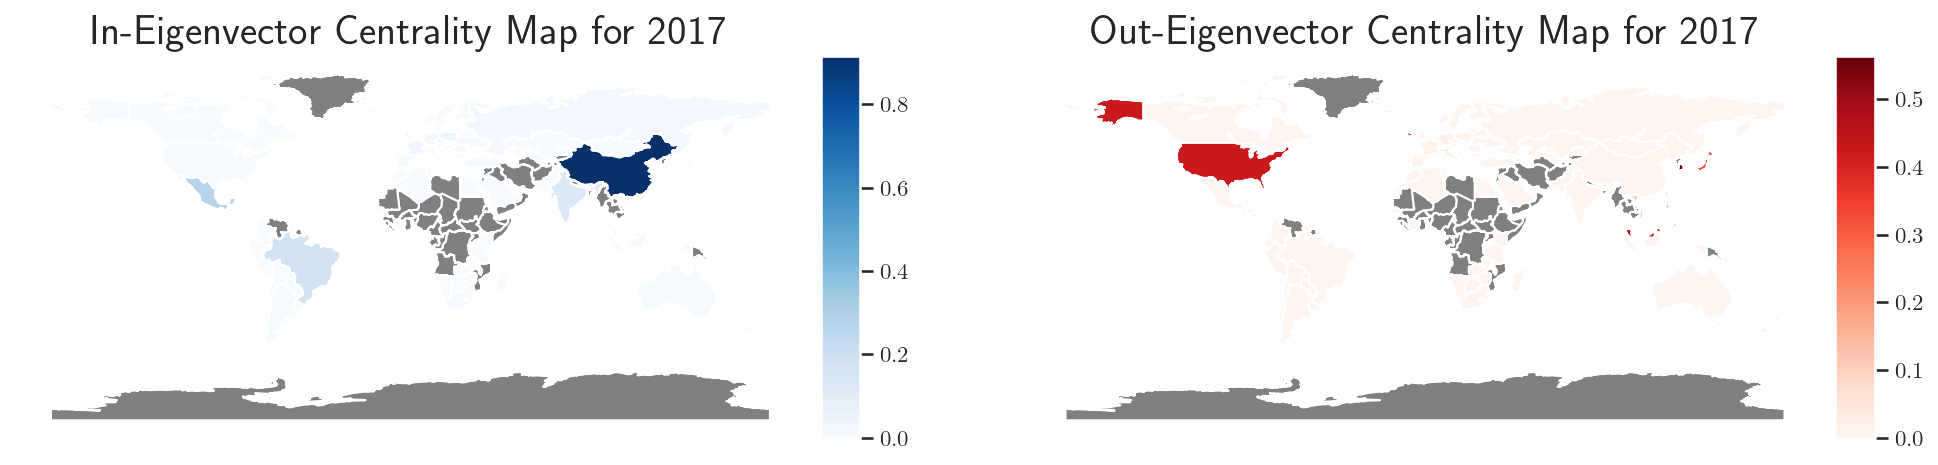
\includegraphics[width=\textwidth]{Fig511-EigenvectorMap.png}
				\caption{In-eigenvector and out-eigenvector centrality maps for the 2017 integrated circuit trade network.}\label{fig:511EigenvectorMap}
			\end{figure}
			
			From Figure \ref{fig:511EigenvectorMap}, we again see that China has a significantly higher in-eigenvector centrality than the rest of the countries, for reasons we have already outlined in the previous sections.
			
			More interestingly, aside from South Korea, the US and many other countries in the East Asian/Southeast Asian regions (including Japan, Malaysia, Singapore and the Philippines) have higher out-eigenvector centralities than average. These are again for reasons that have already been outlined in the previous sections.
			
			\begin{figure}[!h]
				\centering
				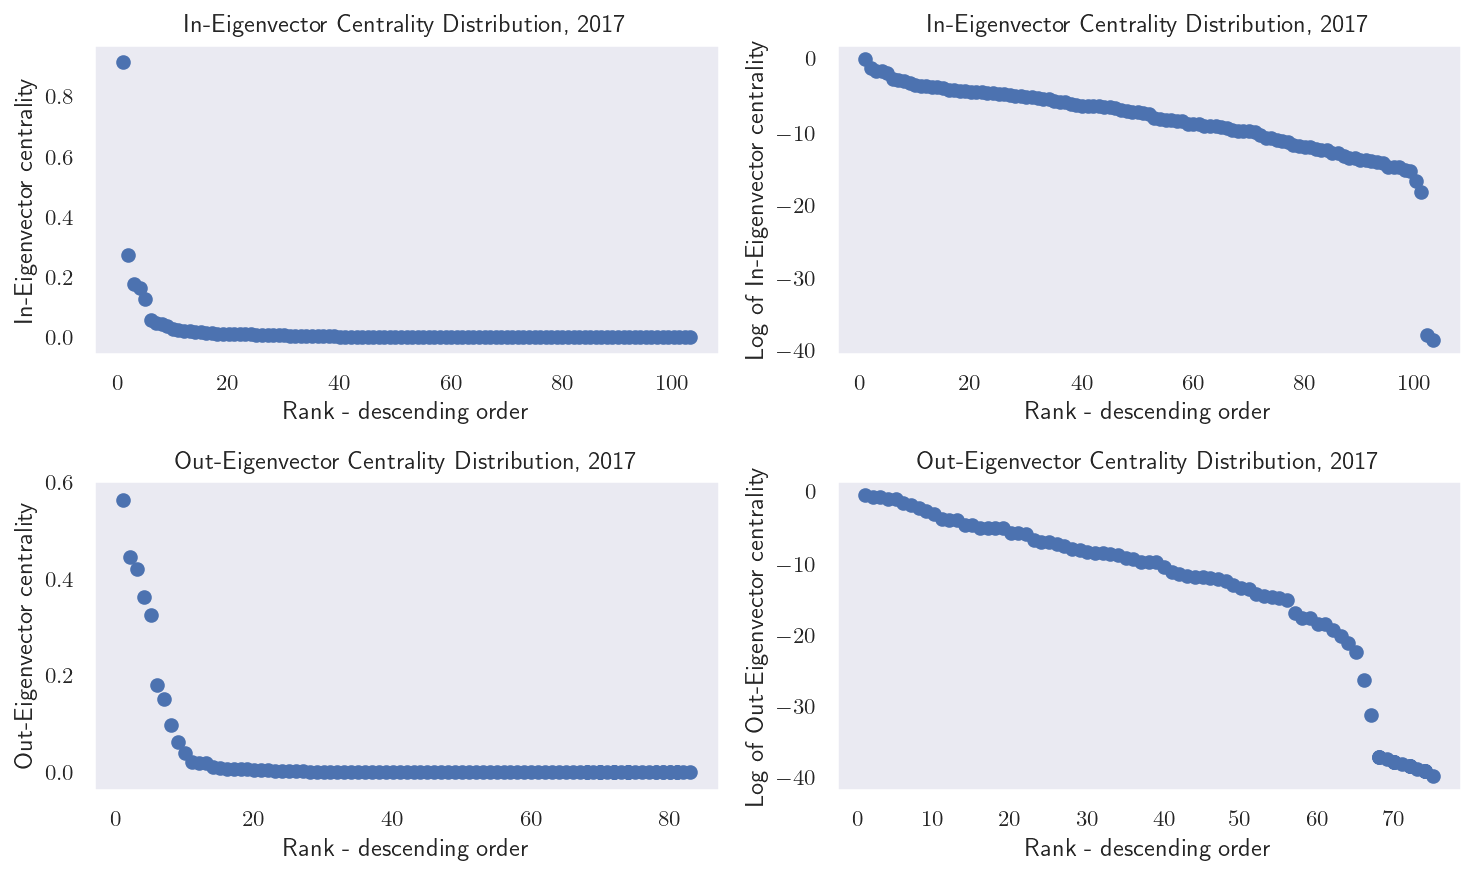
\includegraphics[width=\textwidth]{Fig512-EigenvectorDistribution.png}
				\caption{In-eigenvector and out-eigenvector centrality distributions for the 2017 integrated circuit trade network (linear and semilog).}\label{fig:512EigenvectorDistribution}
			\end{figure}
			
			From Figure \ref{fig:512EigenvectorDistribution}, we find that the outliers become much more apparent in the linear distributions for the eigenvector centralities, again signifying the presence of incoming and outgoing hubs in the trade network that take in/receive a large amount of trade. As before, we find that the semi-log plots are linear, suggesting that eigenvector centrality and the rank are related by an exponential function.
			
			\begin{longtable}{|l|l|r|l|l|r|}
				\caption{Top countries in terms of in-eigenvector and out-eigenvector centrality for the 2017 integrated circuit trade network. \label{tab:tab04TopEigenvector}} \\
				\hline
				\textbf{\small Rank} & \textbf{\small Country} & \textbf{\footnotesize In-eigenvector} & \textbf{\small Rank} &
				\textbf{\small Country} & \textbf{\footnotesize Out-eigenvector} \\
				\hline
				\endfirsthead
				\hline
				\textbf{\small Rank} & \textbf{\small Country} & \textbf{\footnotesize In-eigenvector} & \textbf{\small Rank} &
				\textbf{\small Country} & \textbf{\footnotesize Out-eigenvector} \\
				\hline
				\endhead
				\hline
				\endfoot
				1 & China & 0.9154936928 & 1 & South Korea & 0.5635134302 \\
				2 & Mexico & 0.2743264280 & 2 & Malaysia & 0.4449848880 \\
				3 & Brazil & 0.1760544315 & 3 & USA & 0.4208502627 \\
				4 & Hong Kong & 0.1644362797 & 4 & Ireland & 0.3615903970 \\
				5 & India & 0.1279135329 & 5 & Japan & 0.3245319830 \\
				6 & Czech Republic & 0.0564844672 & 6 & Singapore & 0.1807592182 \\
				7 & The Netherlands & 0.0469685404 & 7 & Philippines & 0.1499541853 \\
				8 & Poland & 0.0422577416 & 8 & Vietnam & 0.0973361937 \\
				9 & France & 0.0351331738 & 9 & Israel & 0.0621369646 \\
				10 & Hungary & 0.0252086984 & 10 & Italy & 0.0382459701 \\
			\end{longtable}
			
			Table \ref{tab:tab04TopEigenvector} reveals that China has the highest in-eigenvector centrality for 2017 while South Korea has the highest out-eigenvector centrality in the same year. This is roughly in line with our earlier results.
			
			In general, a high in-eigenvector centrality suggests that a country's import partners are connected to many other countries which are, in turn, connected to many others. The same is true for the out-eigenvector centrality, except that it concerns a country's export partners.
			
			Overall, based on the centrality measures we computed, we draw the following conclusions:
			
			\begin{itemize}
				\item The results obtained from the degree centrality differs vastly from the results obtained when we consider trade volume (strength centrality), trade volume \& extent of intermediation (betweenness centrality) and trade volume \& importance of trade partners (eigenvector centrality). 
				
				This is apparent in the rank-size distributions, where we can detect the presence of outliers for the latter three centralities.
				
				\item Nonetheless, there is no clear division in the rank-size distributions between core and peripheral nodes. This justifies the use of a distinguishing metric other than centralities to identify core nodes from peripheral ones.
				
				\item China and South Korea consistently have the highest incoming and outgoing weighted centralities, respectively. 
				
				\item Based on the geographical profile of the top countries in terms of the weighted centralities, we can identify three main geographical trading blocs: (i) North America, (ii) Western Europe and (iii) East/Southeast Asia. 
				
				Coincidentally, countries in these regions also have high betweenness centralities, indicating that these regions have a significant midstream presence in the IC trade network.
				
				\item Other notable countries outside these regions include Brazil, India, Poland and Hungary (in terms of in-eigenvector centrality) and Israel (in terms of out-eigenvector centrality).
				
				\item The Philippines has a significant midstream presence in the network. However, it is a much more prominent exporter than importer.
				
			\end{itemize}
			
	\section{Shock Propagation (Supply-Side Decrease)}
	\label{sec:53supplysideDecrease}
	
	We can now use the model outlined in Chapter 4 to evaluate how perturbing different nodes will affect the network, using the three metrics discussed to measure these effects. Because we have two variable parameters (the shock and spread parameter), we averaged the results across different values of the parameters, considering values from 0 to 1 in increments of 0.1 for both the shock and spread parameter. 
	
	As such, we get the cascade depth, cascade size and exposure for the nodes on average. Unless explicitly stated, the results that will follow will be on average.
	
		\subsection{Cascade Size and Cascade Depth}
		\label{ssec:531cascadeSizeDepth}
		
			\subsubsection{Geographic Distribution}
			\label{ssec:5311geographic}
			
				\begin{figure}[!h]
					\centering
					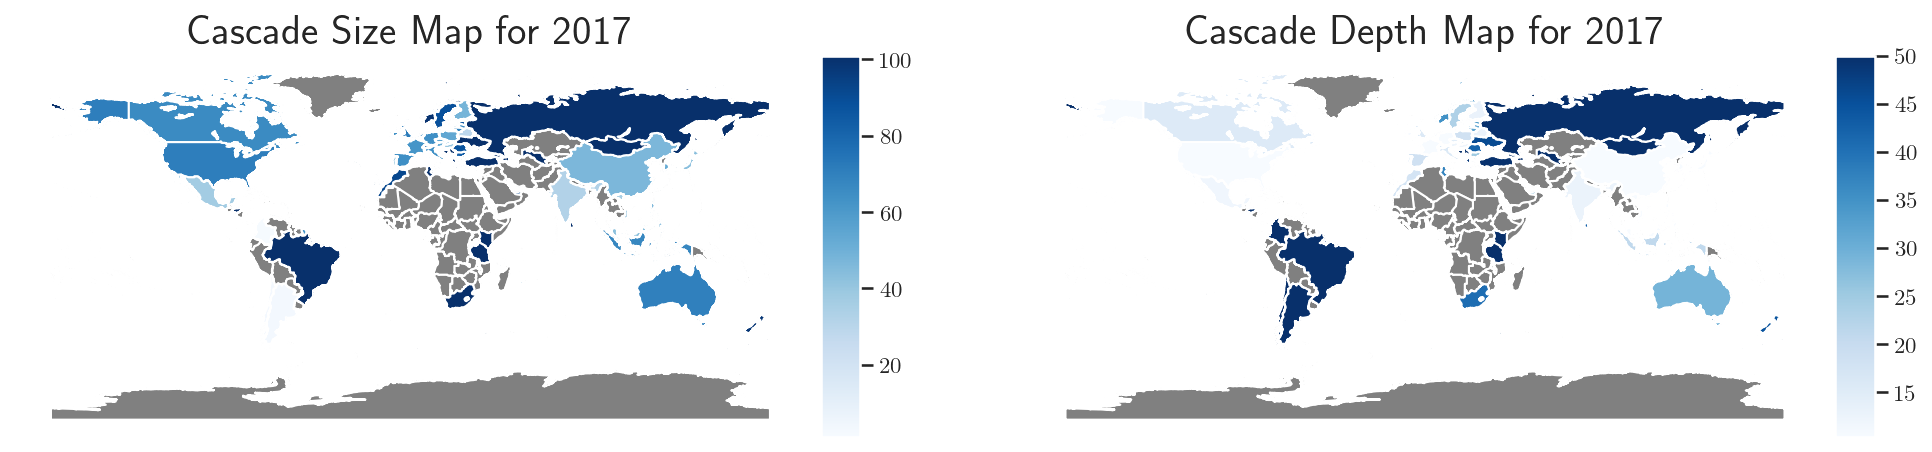
\includegraphics[width=\textwidth]{Fig513-CascadeMap.png}
					\caption{Cascade size and cascade depth maps for the 2017 integrated circuit trade network.}\label{fig:513CascadeMap}
				\end{figure}
				
				Figure \ref{fig:513CascadeMap} depicts the associated cascade size and cascade depth for each country. We notice the following patterns.
				
				Note that the North American (particularly Canada and the US), Western European, Southeast Asian and East Asian regions are associated with a high cascade size but low cascade depth, meaning that shocks that start in these areas only take a few iterations to finish but pervade a large portion of the network.
				
				In contrast, many of the countries in the CIS and Eastern European regions are associated with both high cascade size and high cascade depth, meaning that shocks that start here take a long time to finish (and may not even terminate within 50 iterations) but reach most of the nodes in the network. 
				
				In keeping with our core-periphery hypothesis, we can surmise that countries which are associated with low cascade depths on average can probably be said to be \textit{core} nodes, as shocks to them only take a few iterations to terminate. Nodes that are associated with high cascade depths can then be said to be \textit{peripheral} nodes, since shocks to these nodes do not significantly affect the nodes in the network. From the map, however, there does not seem to be a sharp core-periphery divide.
				
				Furthermore, note that compared to the CIS/Eastern European countries, some of the countries in the South American regions are also associated with low cascade size and high cascade depth. This signifies that not only do the shocks take a long time to finish (In fact, the shock may not even terminate within 50 iterations) but they also do not pervade the network significantly. These must be isolated nodes which lie in the periphery of the IC trade network.
				
				As such, we can further classify the nodes into whether shocks to them affect the entire network (\textit{connected} nodes) or only a select few (\textit{isolated} nodes). However, the divide between connected and isolated nodes is even less sharp, much more so for core nodes.
	
			\subsubsection{Distribution based on Shock and Spread Parameters}
			\label{ssec:5312shockspread}
			
				\begin{figure}[!h]
					\centering
					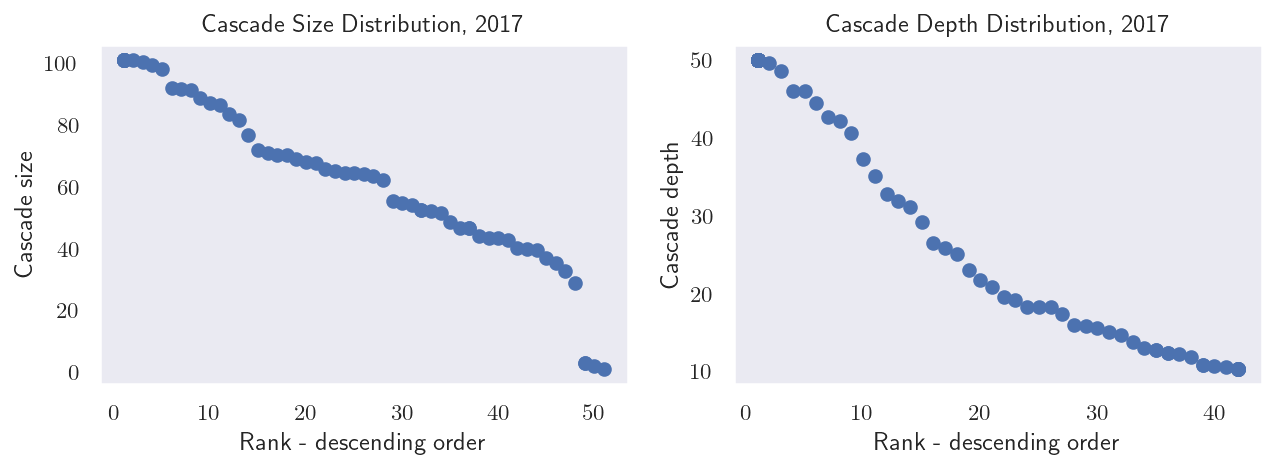
\includegraphics[width=\textwidth]{Fig514-CascadeDistribution.png}
					\caption{Cascade size and cascade depth distribution for the 2017 integrated circuit trade network (averaged).}\label{fig:514CascadeDistribution}
				\end{figure}
			
				From the geographic distribution, we surmised that we can potentially use cascade depth as a distinguishing metric. To check if this is the case, we plot the rank-size distributions for cascade size and cascade depth, shown in Figure \ref{fig:514CascadeDistribution}. The plots show that both the cascade size and cascade depth are somewhat uniformly distributed across the range of values over which they occur. Both are also roughly linear, suggesting that the rank and the cascade size/depth on average are linearly related. 
				
				These results might seem to contradict the core-periphery hypothesis that we had earlier posited. However, because we averaged the results across all shock and spread parameters in our selected parameter space, the uniformity may simply be due to this averaging. To check, we run the simulation for shock and spread parameters of 0.1, 0.5 and 0.9 and check the cascade size and depth distributions for each simulation. 
				
				\begin{figure}[!h]
					\centering
					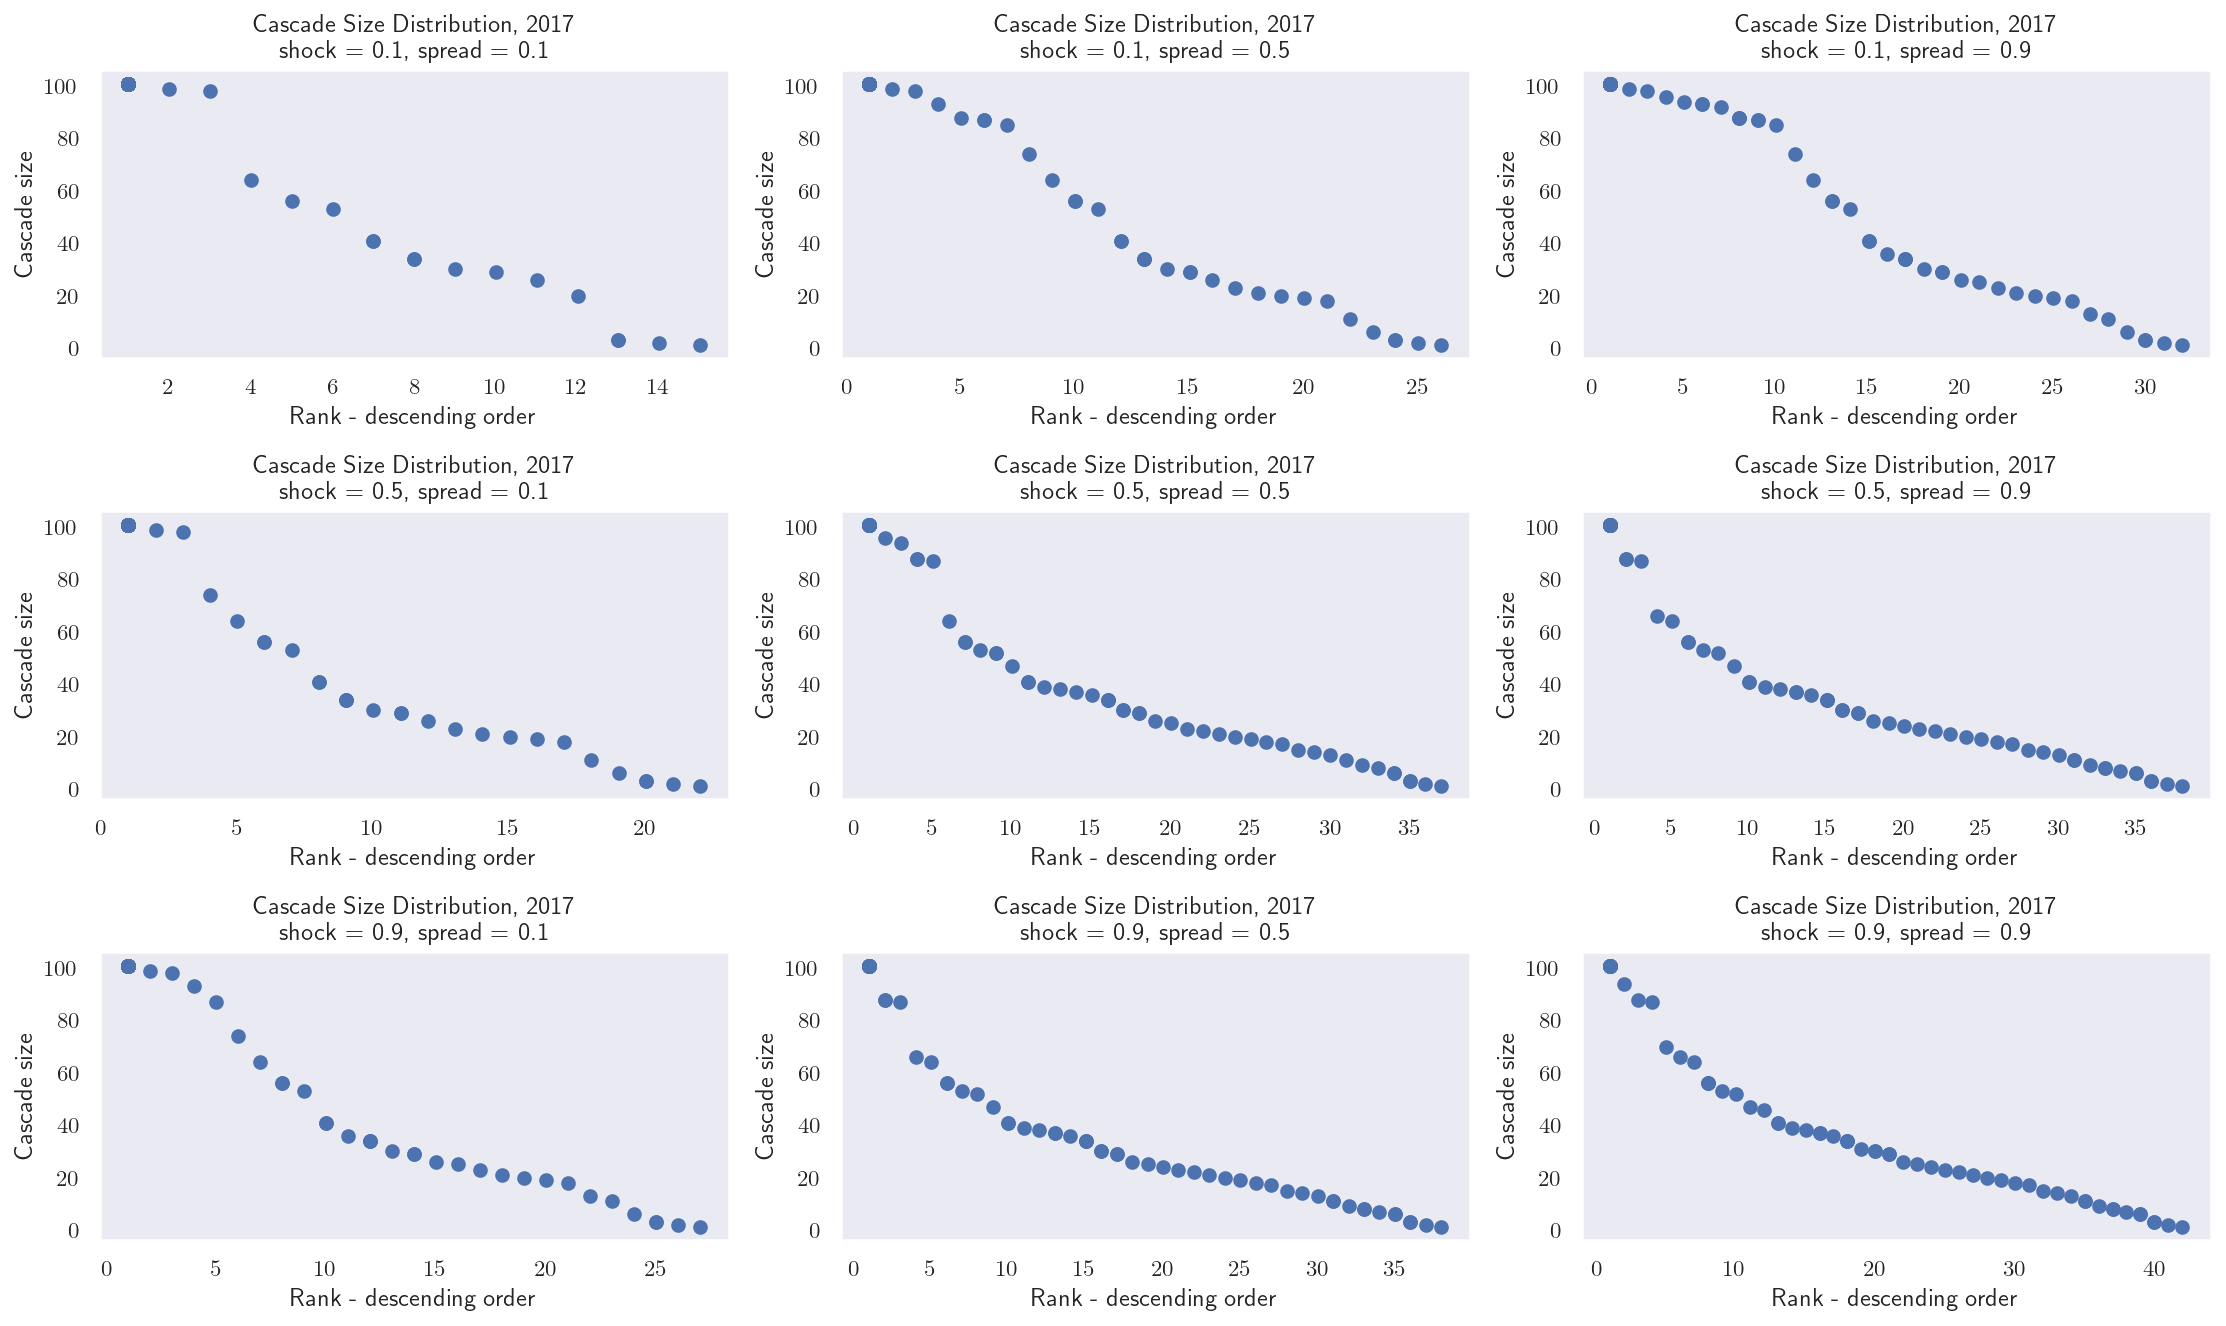
\includegraphics[width=\textwidth]{Fig515-CascadeSizeDistribution.png}
					\caption{Cascade size distribution for the 2017 integrated circuit trade network for different shock and spread parameters.}\label{fig:515CascadeSizeDistribution}
				\end{figure}
			
				\begin{figure}[!h]
					\centering
					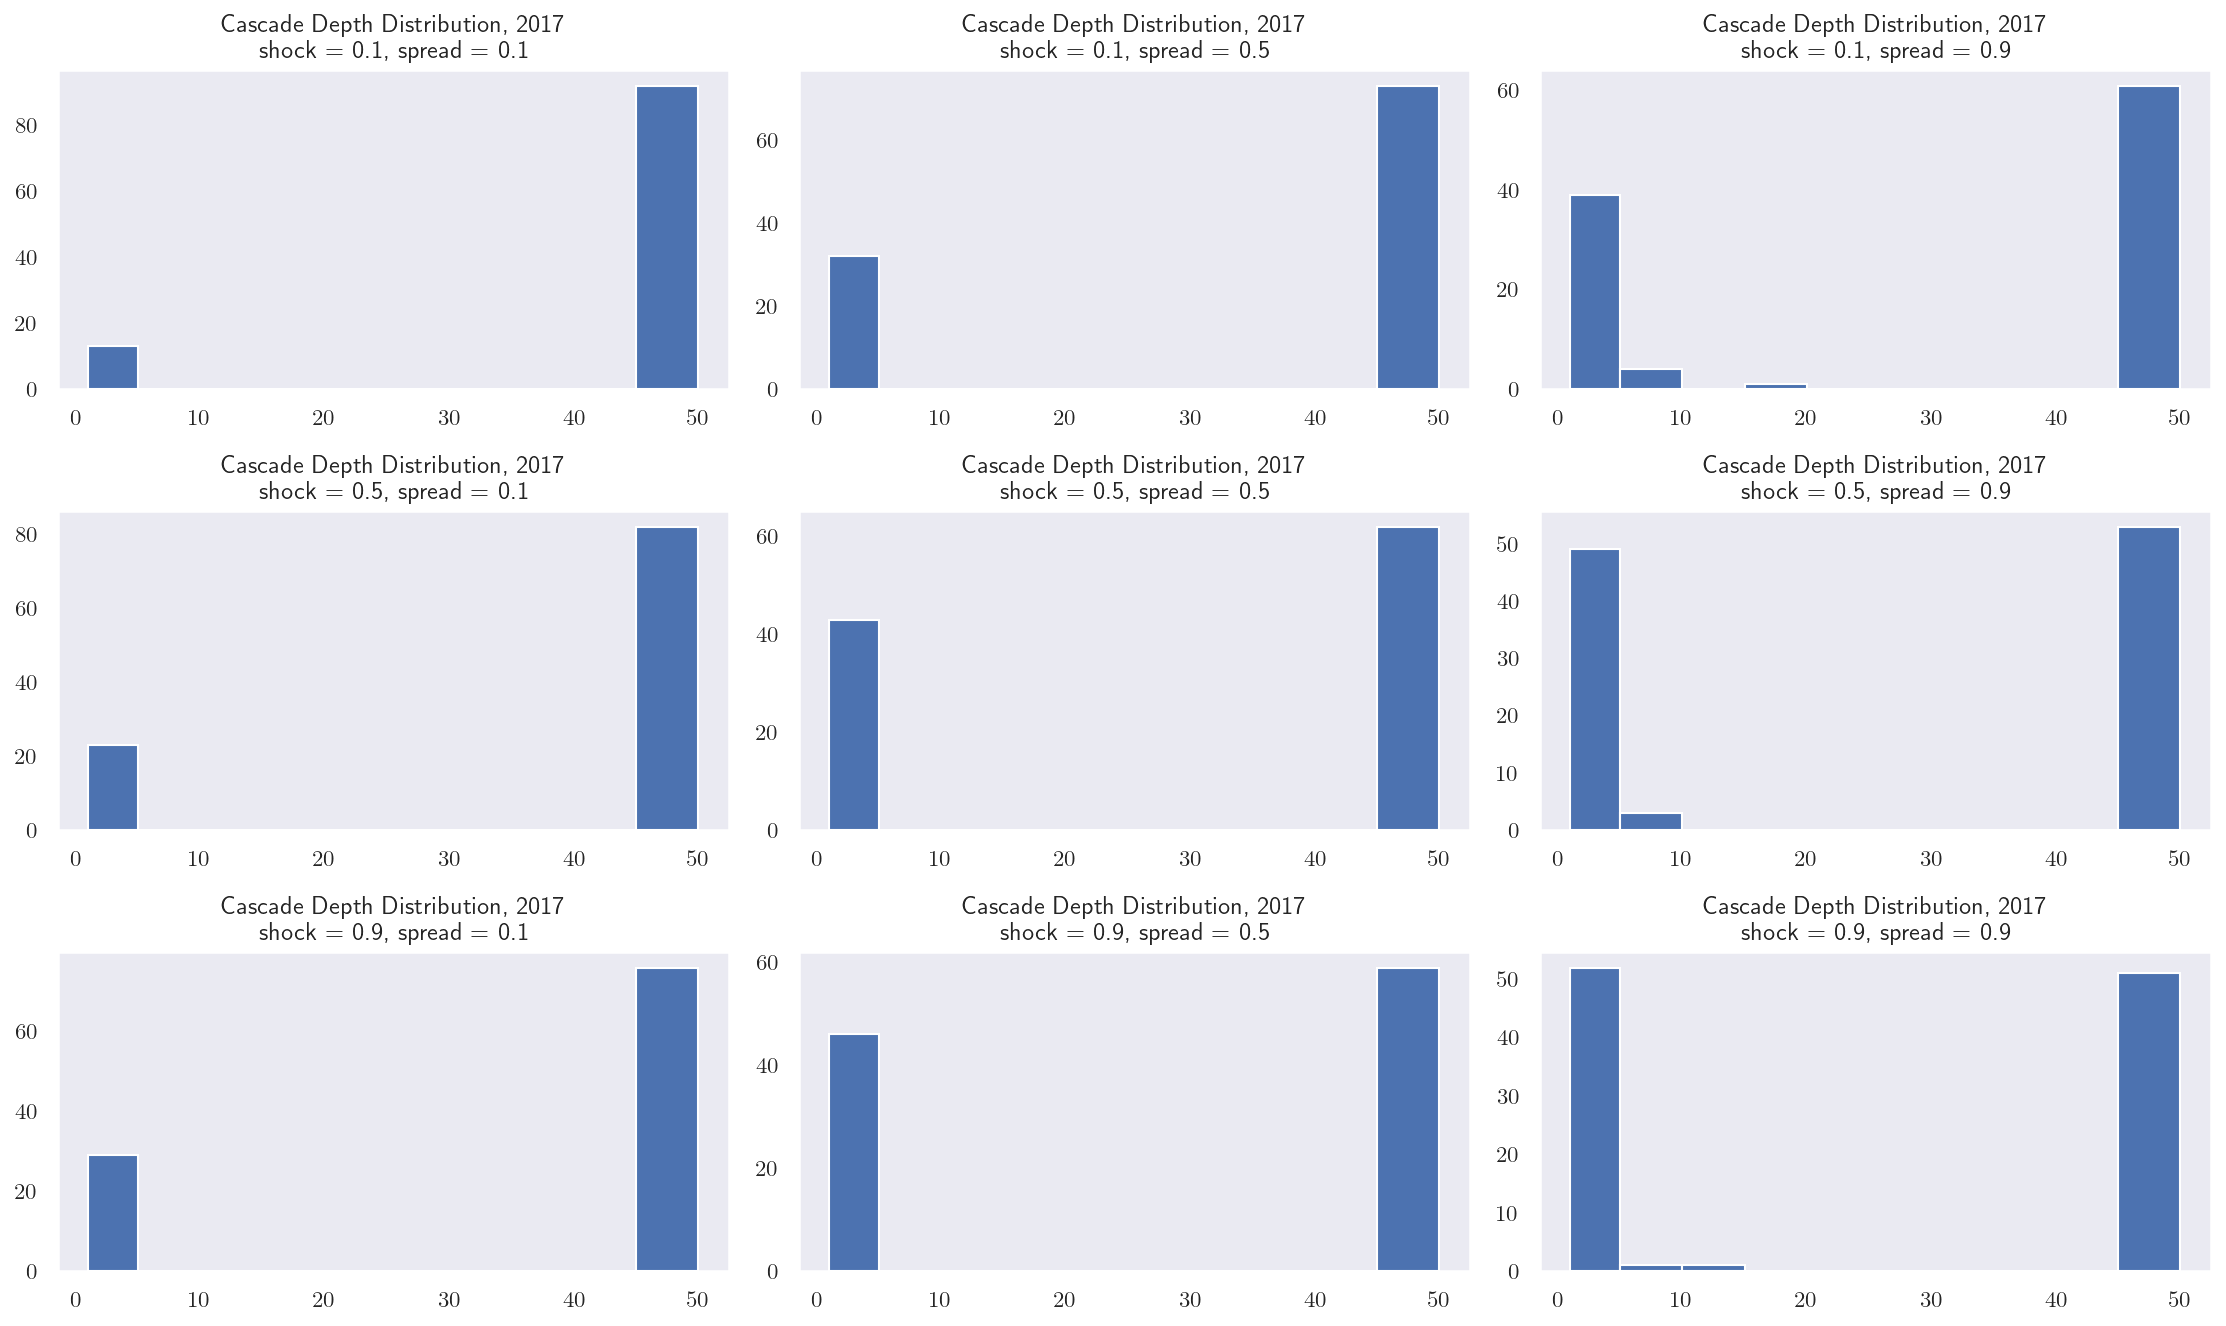
\includegraphics[width=\textwidth]{Fig516-CascadeDepthDistribution.png}
					\caption{Cascade depth distribution for the 2017 integrated circuit trade network for different shock and spread parameters}\label{fig:516CascadeDepthDistribution}
				\end{figure}
				
				The results are shown in Figures \ref{fig:515CascadeSizeDistribution} and \ref{fig:516CascadeDepthDistribution}. We see from Figure \ref{fig:515CascadeSizeDistribution} that as we increase the shock and spread parameters, the cascade size begins taking on the shape of the distribution in the averaged variant from earlier. Thus, the distribution of the averaged cascade size seems to be somewhat representative of the cascade size distribution for arbitrary values of the shock and spread parameter.
				
				The same is not true for the cascade depth, however. Note that the histograms in Figure \ref{fig:516CascadeDepthDistribution} have bin edges which are multiples of 5 (Thus, the bins are from 0 to 5, 5 to 10, and so on).
				
				From the figure, we observe a roughly bimodal distribution for cascade depth, with the first mode corresponding to influential countries where the simulation ends early and the second mode corresponding to countries for which the simulation does not terminate after 50 iterations.
				
				Furthermore, notice that as we increase either the shock or spread parameter, nodes begin "jumping" from the right bin to the left bin. This is intuitively sound, as increasing either the shock or spread parameter increases the size and the extent of the shock, respectively, which leads to the simulation terminating/requiring less iterations to terminate. It is these nodes "jumping" from one bin to the other which leads to the relative uniformity of the averaged cascade depth distribution that we had seen earlier. The bimodality in cascade depth lends better credence to our core-periphery hypothesis and will enable us to designate nodes as core or peripheral.
				
				To check, we also plot cascade depth against cascade size. Similar to what we did earlier, we restrict the parameter space to the set of values 0.1, 0.5 and 0.9 and run the simulation for these values to get a better picture of how cascade size and depth vary in relation to each other.
				
				\begin{figure}[!h]
					\centering
					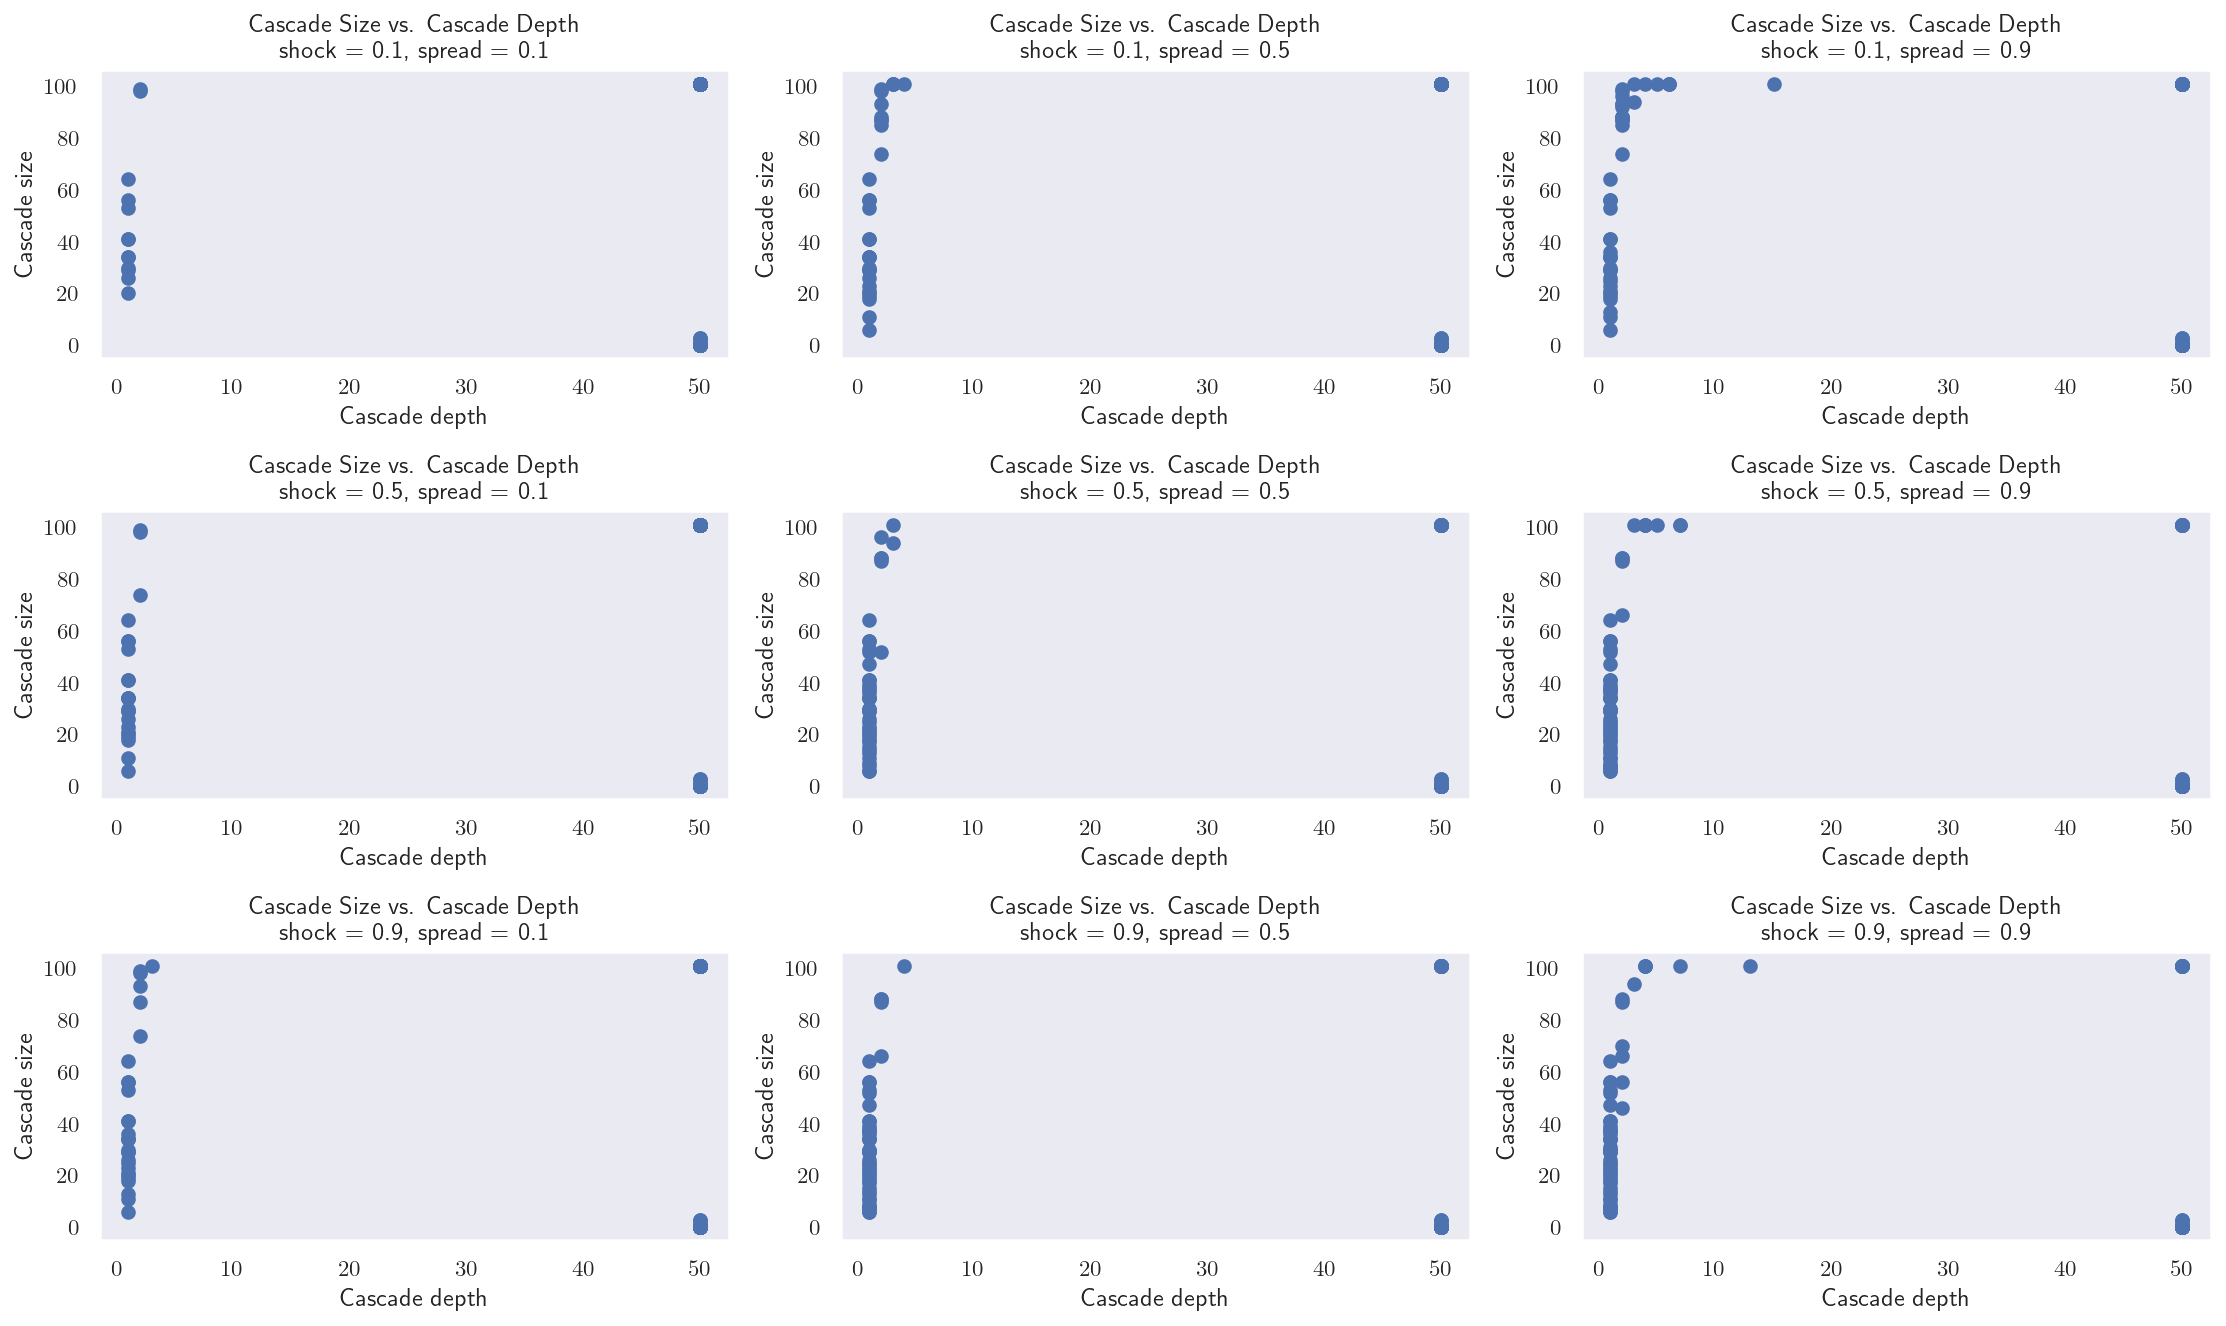
\includegraphics[width=\textwidth]{Fig517-CascadeSizevsDepth.png}
					\caption{Cascade size vs. cascade depth for the 2017 integrated circuit trade network for different shock and spread parameters}\label{fig:517CascadeSizevsDepth}
				\end{figure}
				
				As before, looking at Figure \ref{fig:517CascadeSizevsDepth}, we see a clear divide between core and peripheral nodes for all cases with respect to cascade depth. Furthermore, increasing either parameter leads to nodes from the right side of the graph "migrating" to the left side. 
				
				More notably, though, we also see a divide between peripheral nodes in terms of cascade size. Setting some peripheral nodes as the starting node results in the simulation affecting only a select number of nodes despite it never terminating. For the other peripheral nodes, however, the simulation ends up affecting almost the entire network. This is in line with the connected vs. isolated node distinction that we made earlier. This distinction does not seem to be especially marked among the core nodes, however. While this distinction undoubtedly exists, though, it does not seem to be particularly important.

			\subsubsection{Identifying Core and Peripheral Nodes}
			\label{ssec:5313coreperiphery}			
				We can now designate each node as either a core or peripheral node. As we can see from Figures \ref{fig:516CascadeDepthDistribution} and \ref{fig:517CascadeSizevsDepth}, however, the designation depends on the value of both the shock and spread parameter. To get around this problem, we follow Li et al. (2014) and compute for the minimum value of the shock parameter required to designate a node as a core node, setting the spread parameter equal to 1. This decision is reasonable, as the spread parameter only accounts for the amount of "friction" present in the shocks, to make a physical analogy. Ideally, we would like to examine the "frictionless" case.
				
				In this case, we define a \textit{core node} as one which requires at most 10 iterations to terminate, which is consistent with Figures \ref{fig:516CascadeDepthDistribution} and \ref{fig:517CascadeSizevsDepth}. The shock parameter is computed using a modified bisection search algorithm which is run for 100 iterations, during which the computed values for the minimum shock parameter have been found to converge.
				
				After this, we rank the nodes based on the minimum shock parameter. We can then set a threshold shock parameter and designate all countries with a smaller minimum shock parameter as core nodes, with the rest being designated as peripheral nodes.
				
				\begin{figure}[!h]
					\centering
					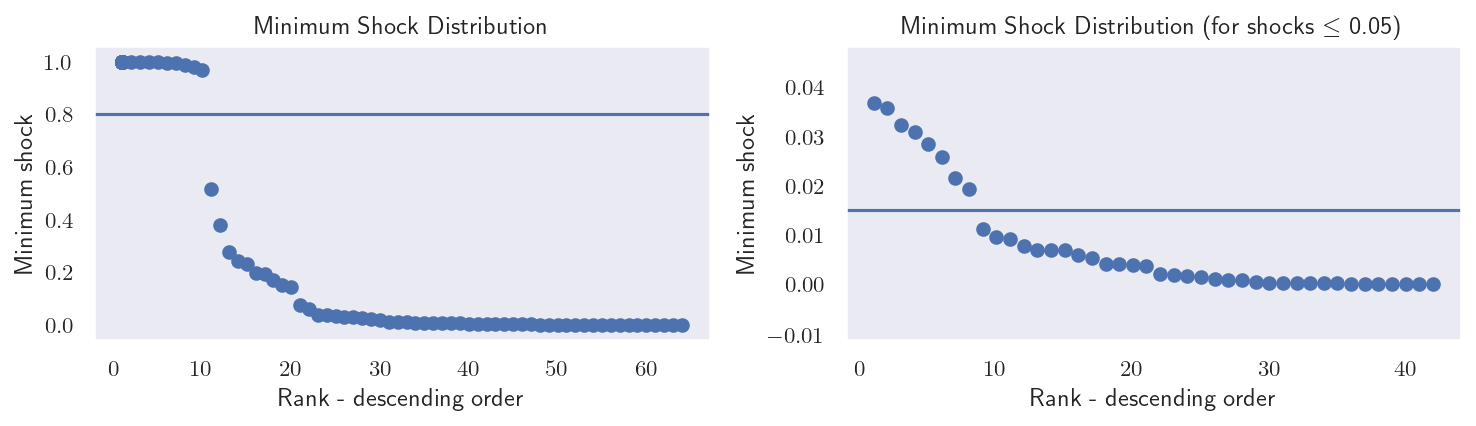
\includegraphics[width=\textwidth]{Fig518-MinimumShock.png}
					\caption{Minimum shock  distribution for the 2017 integrated circuit trade network}\label{fig:518MinimumShock}
				\end{figure}
			
				From Figure \ref{fig:518MinimumShock}, we see a clear gap between the minimum shock values for core and peripheral nodes. We set a threshold value of 0.8 to distinguish between these two groups.
				
				Note however that in doing so, we end up with a largely heterogeneous core, with a large variance in the minimum shock value. Thus, in the interest of keeping as tight a core as possible, we drill down on the values and check for significant gaps. Plotting minimum shock values that are less than 0.05, we find a significant gap at a shock value of around 0.015.
				
				Thus, we end up with two thresholds at 0.8 and 0.015. Those with a minimum shock value higher than 0.8 form the periphery of our outgoing network, meaning that the failure of any one of these countries does not significantly affect the outgoing network at all. Those with a minimum shock value lower than 0.015 form the inner core and the failure of any one of these countries carries with it a significant amount of systemic risk.
				
				Furthermore, those countries that have minimum shock values in between the two occupy an intermediate position of the network and form the outer core. These countries may be valuable to look at, as the effect of their failure may be mitigated by similarly positioned nodes coming in to "substitute" for them.
								 
				\begin{figure}[!h]
					\centering
					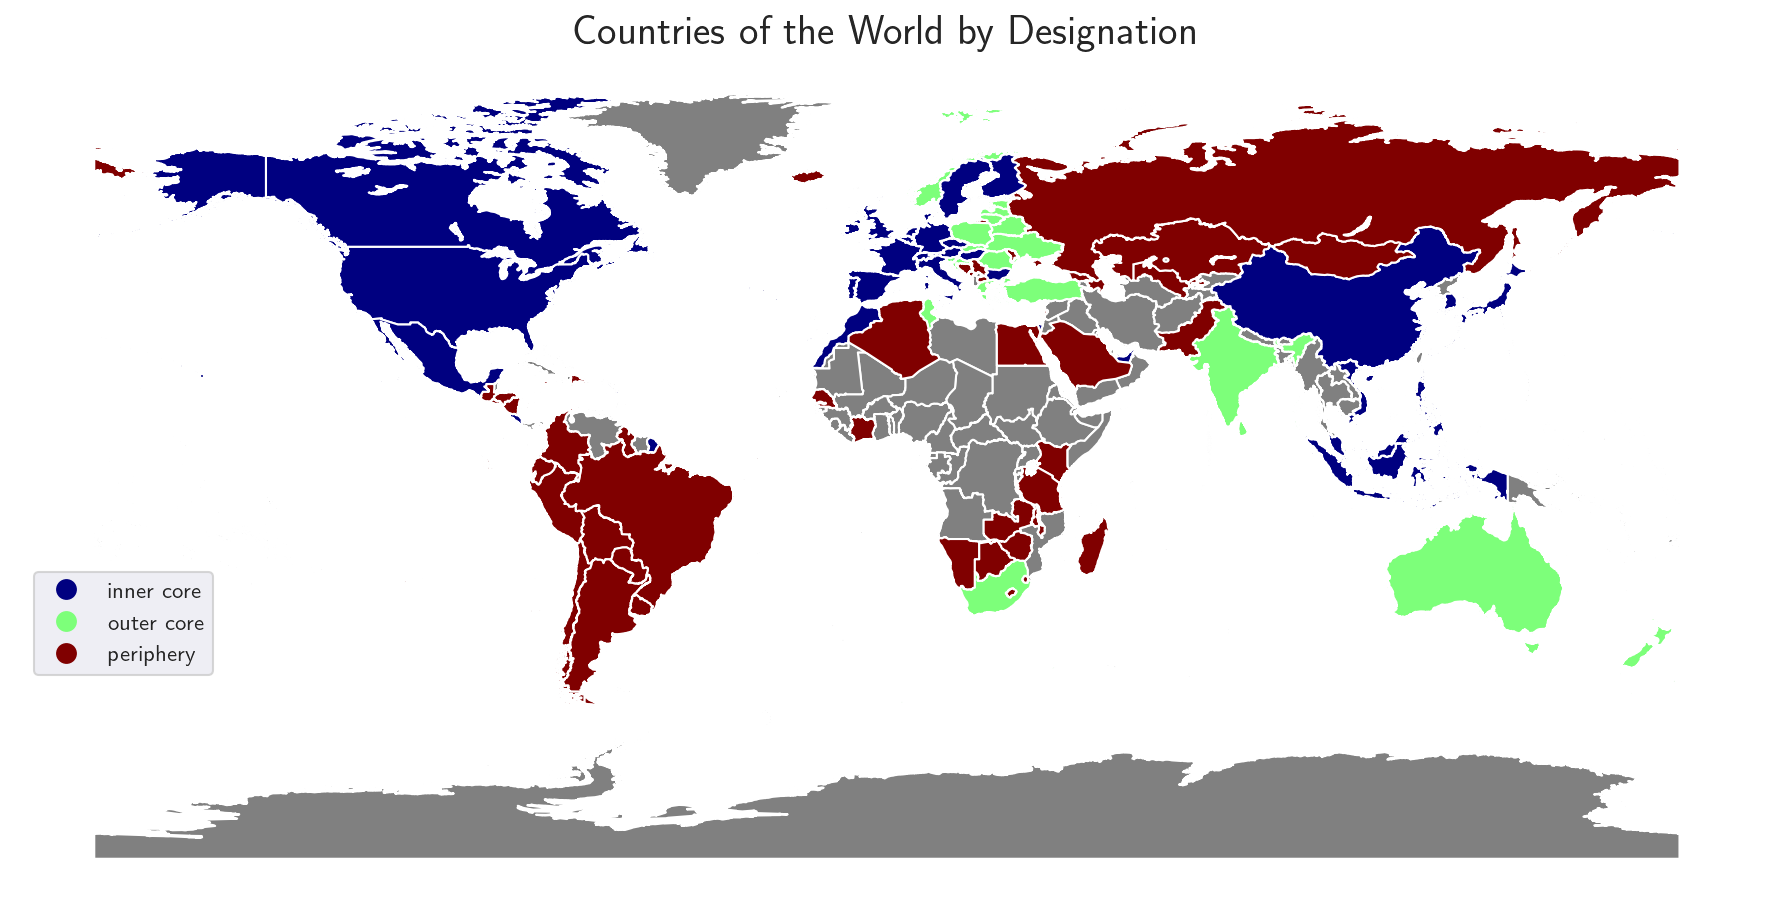
\includegraphics[width=\textwidth]{Fig519-CorePeripheryMap.png}
					\caption{Core-periphery map for the 2017 integrated circuit trade network}\label{fig:519CorePeripheryMap}
				\end{figure}
				 
				We can visualize the geographic distribution of core and peripheral nodes using a choropleth map, as in Figure \ref{fig:519CorePeripheryMap}.
				
				In line with earlier observations, the Southeast Asian/East Asian region is a major hub in the IC trade network, along with North America and Western Europe. Other notable inner core countries include Spain, Portugal, Morocco, Sweden and Finland. As such, these regions are the most susceptible to systemic risk pertinent to events which are related to a supply-side decrease.
				
				The core is often comprised of central and densely connected nodes, while the periphery consists of sparsely connected nodes that are linked to the core. Often, this implies that there must be a significant number of core-core and core-periphery links but not much periphery-periphery links. We examine if this is the case with the core and the periphery.
				
				To do so, we look at a number of metrics to characterize inner core and peripheral nodes. At the node level, these include: (1) average out-degree centrality, (2) average out-strength centrality, (3) average betweenness centrality and (4) average out-eigenvector centrality. At the edge level, these include: (1) average link weight and (2) normalized number of links.
				
				\begin{longtable}{|l|r|r|r|r|}
					\caption{Average centrality based on designation. \label{tab:tab05AverageCentrality}} \\
					\hline
					& \textbf{\small out-degree} & \textbf{\small out-strength} & \textbf{\small betweenness} &
						\textbf{\small out-eigenvector} \\ 
					\hline
					\endfirsthead
					\hline
					& \textbf{out-degree} & \textbf{out-strength} & \textbf{betweenness} &
					\textbf{out-eigenvector} \\ 
					\hline
					\endhead
					\hline
					\endfoot
					inner core &  	31.9411764706 & 0.0293792128 & 0.0566571849 & 0.0808870910 \\
					outer core &  	9.4000000000 & 0.0000542109 & 0.0078883495 & 0.0000885774 \\
					peripheral & 0.6470588235  & 0.0000004421 & 0.0003148384 & 0.0000002294 \\
				\end{longtable}
				
				From Table \ref{tab:tab05AverageCentrality}, we find that inner core nodes tend to be associated with significantly higher out-degrees, higher out-strength centralities, higher betweenness centralities and higher out-eigenvector centralities relative to outer core and peripheral nodes. These reflect their greater importance in the network of outgoing links and the increased systemic risk coupled with it.
				
				\begin{longtable}{|l|l|r|r|}
					\caption{Edge-level metrics based on designation. \label{tab:tab06EdgeLevel}} \\
					\hline
					\multicolumn{1}{|c|}{\textbf{\small source}} & \multicolumn{1}{|c|}{\textbf{\small target}} & \multicolumn{1}{|c|}{\textbf{\small average}} & \textbf{\small normalized number} \\ 
					\multicolumn{1}{|c|}{\textbf{\small designation}} & \multicolumn{1}{|c|}{\textbf{\small designation}} & \multicolumn{1}{|c|}{\textbf{\small link weight}} & \multicolumn{1}{|c|}{\textbf{\small of links}} \\ 
					\hline
					\endfirsthead
					\hline
					\multicolumn{1}{|c|}{\textbf{\small source}} & \multicolumn{1}{|c|}{\textbf{\small target}} & \multicolumn{1}{|c|}{\textbf{\small average}} & \textbf{\small normalized number} \\ 
					\multicolumn{1}{|c|}{\textbf{\small designation}} & \multicolumn{1}{|c|}{\textbf{\small designation}} & \multicolumn{1}{|c|}{\textbf{\small link weight}} & \multicolumn{1}{|c|}{\textbf{\small of links}} \\ 
					\hline
					\endhead
					\hline
					\endfoot
					inner core & inner core & 487629051.7773476839 & 0.4509803922 \\
					inner core & outer core & 17290735.2508352734 & 0.5720588235 \\
					inner core & peripheral & 22518608.0633187629 & 0.1101499423 \\
					outer core & inner core & 1647297.7182290393
					 & 0.1058823529 \\
					outer core & outer core & 855478.9668428004
					 & 0.2131578947 \\
					outer core & peripheral & 2625335.8017947599
					& 0.0343137255 \\
					peripheral & inner core & 54008.1614258817 & 0.0057670127 \\
					peripheral & outer core & 53862.5882848540 & 0.0049019608 \\
					peripheral & peripheral & 278268.5568675100 & 0.0070588235 \\
				\end{longtable}
			
				From Table \ref{tab:tab06EdgeLevel}, we find that inner core-inner core links tend to have significantly higher weights on average compared to the rest. Moreover, inter-inner core links tend to be relatively more frequent, with around 45\% of all possible core-core links actually in the network. Note too the hierarchy with respect to the source designation: outgoing links from the inner core tend to have higher trade volume and tend to occur more frequently, followed by outgoing links from the outer core, then outgoing links from the periphery. This further reinforces the existence of a core-periphery structure in the trade of outgoing links.
				
		\subsection{Exposure}
		\label{ssec:532exposure}
		
		\begin{longtable}{|l|l|r|l|l|r|}
			\caption{Top countries in terms of exposure with respect to the Philippines for the 2017 integrated circuit trade network. \label{tab:tab07Exposure1}} \\
			\hline
			\textbf{\small Rank} & \textbf{\small Country} & \multicolumn{1}{|c|}{\textbf{\small Exposure}} & \textbf{\small Rank} &
			\textbf{\small Country} & \multicolumn{1}{|c|}{\textbf{\small Exposure}} \\
			&  & \multicolumn{1}{|c|}{\textbf{\small given}} & & & \multicolumn{1}{|c|}{\textbf{\small received}} \\  
			\hline
			\endfirsthead
			\hline
			\textbf{\small Rank} & \textbf{\small Country} & \multicolumn{1}{|c|}{\textbf{\small Exposure}} & \textbf{\small Rank} &
			\textbf{\small Country} & \multicolumn{1}{|c|}{\textbf{\small Exposure}} \\
			&  & \multicolumn{1}{|c|}{\textbf{\small given}} & & & \multicolumn{1}{|c|}{\textbf{\small received}} \\  
			\hline
			\endhead
			\hline
			\endfoot
			1 & Hong Kong & 0.1502006133 & 1 & Belgium & 0.0858804018 \\
			2 & China & 0.1064487653 & 2 & Italy & 0.0326583391 \\
			3 & Singapore & 0.0605339492 & 3 & Czech Republic & 0.0298521031 \\
			4 & Germany & 0.0279158430 & 4 & USA & 0.0167613309 \\
			5 & The Netherlands & 0.0164048518 & 5 & South Korea & 0.0148975621 \\
			6 & Mexico & 0.0101674301 & 6 & Tunisia & 0.0120685283 \\
			7 & Malaysia & 0.0083895435 & 7 & Japan & 0.0068295375 \\
			8 & Vietnam & 0.0069181383 & 8 & Norway & 0.0061298939 \\
			9 & France & 0.0067937776 & 9 & Israel & 0.0030431331 \\
			10 & Canada & 0.0022847275 & 10 & Morocco & 0.0023936015 \\
		\end{longtable}
		
		We find that the Philippines affects Hong Kong the most, with Hong Kong being exposed to 15.02\% of the shock from the Philippines on average. Meanwhile, Belgium affects the Philippines the most, with the country being exposed to 8.59\% of the shocks from Belgium on average.
		
	\section{Shock Propagation (Supply-Side Increase)}
	\label{sec:54supplysideIncrease}
	
	We developed an analogous model in Chapter 4 corresponding to a supply-side increase. In this section, we will use the three metrics discussed to measure the effects of perturbing each node in the network in accordance with this model of supply-side increase. Once again, we averaged the results across different values of the parameters, considering values from 0 to 1 in increments of 0.1 for both the shock and spread parameter. Unless explicitly stated, the results that will follow will be on average.
	
	\subsection{Cascade Size and Cascade Depth}
	\label{ssec:541cascadeSizeDepth}
	
	\subsubsection{Distribution of Cascade Size and Depth}
	\label{ssec:5411distribution}
	
	\begin{figure}[!h]
		\centering
		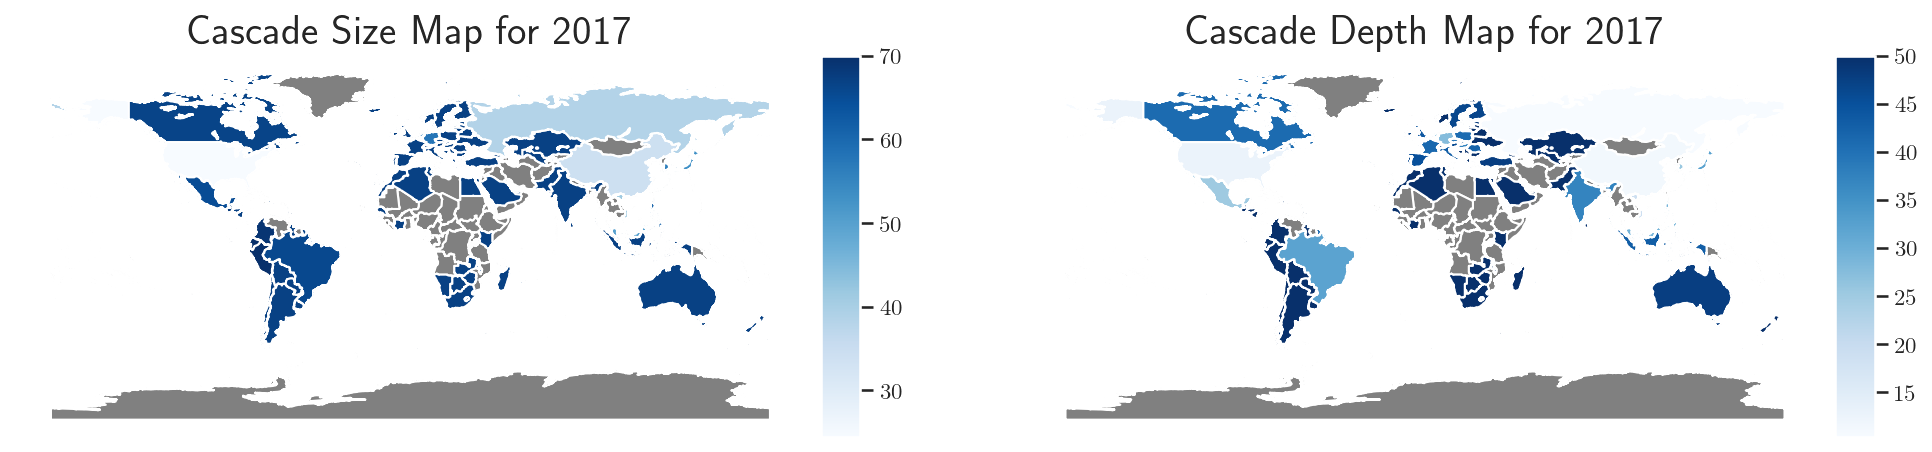
\includegraphics[width=\textwidth]{Fig520-CascadeMap.png}
		\caption{Cascade size and cascade depth maps for the 2017 integrated circuit trade network.}\label{fig:519CascadeMap}
	\end{figure}
	
	Figure \ref{fig:519CascadeMap} depicts the associated cascade size and cascade depth for each country. We notice the following patterns.
	
	Some countries in Southeast Asia/East Asia and Western Europe have a high cascade size and low cascade depth. Most other countries, however, are associated with both high cascade size and high cascade depth. This signifies that shocks in these countries take a long time to finish but reach most of the nodes in the network.
	
	In line with our core-periphery hypothesis, the former countries probably constitute the core of the network, while the latter countries must be nodes in the periphery of the IC trade network which are themselves connected to a number of well-connected nodes, allowing shocks to these countries to spread to most of the network. 
	
	Similar to what we did earlier, we also plot cascade size vs. cascade depth, restricting the parameter space to the set of values 0.1, 0.5 and 0.9.
	
	\begin{figure}[!h]
		\centering
		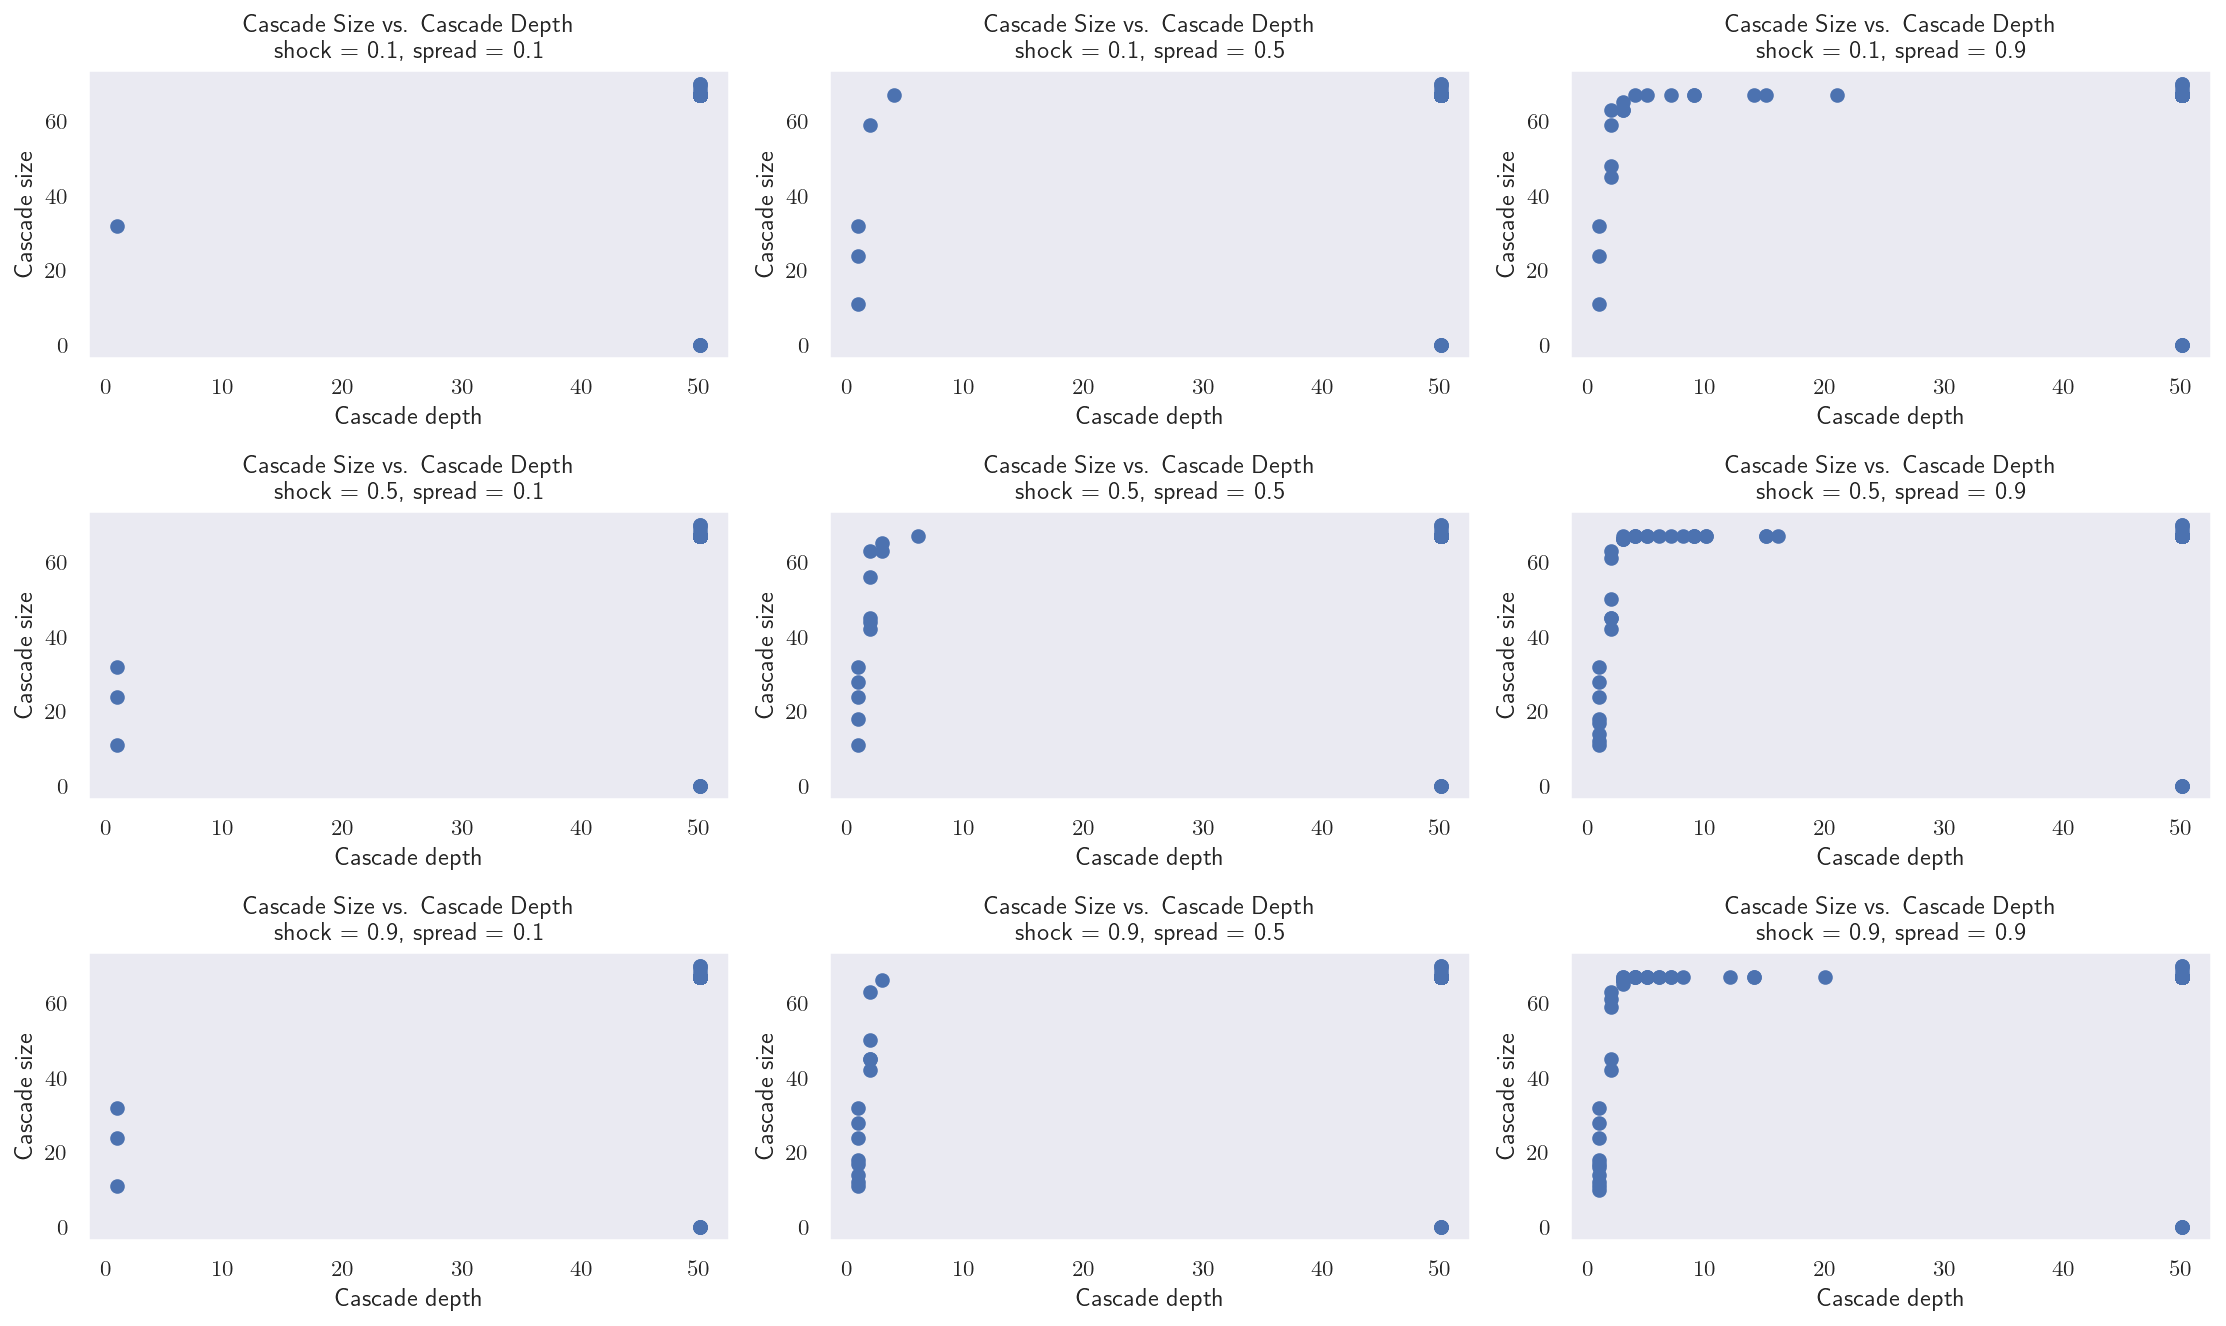
\includegraphics[width=\textwidth]{Fig521-CascadeSizevsDepth.png}
		\caption{Cascade size vs. cascade depth for the 2017 integrated circuit trade network for different shock and spread parameters.}\label{fig:520CascadeSizevsDepth}
	\end{figure}
	
	Once again, from Figure \ref{fig:520CascadeSizevsDepth}, we see a clear divide between core and peripheral nodes for all cases with respect to cascade depth. Moreover, increasing either the shock or spread parameter causes nodes from the right side to move to the left. This makes sense, as increasing the shock/spread parameter increases the size/extent of the shock, leading to less iterations towards the terminating condition in general. 
	
	\subsubsection{Identifying Core and Peripheral Nodes}
	\label{ssec:5412coreperiphery}		
	We can now designate each node as either a core or peripheral node. Following Li et al. (2014), we compute for the minimum value of the shock parameter required to designate a node as a core node, setting the spread parameter equal to 1. This decision is reasonable, as the spread parameter only accounts for the amount of "friction" present in the shocks, to make a physical analogy. Ideally, we would like to examine the "frictionless " case.
	
	In this case, we define a \textit{core node} as one which requires at most 10 iterations to terminate, consistent with Figure \ref{fig:520CascadeSizevsDepth}. The shock parameter is computed using a modified bisection search algorithm which is run for 100 iterations, during which the computed values for the minimum shock parameter have been found to converge.
	
	After this, we rank the nodes based on the minimum shock parameter. We can then set a threshold shock parameter and designate all countries with a smaller minimum shock parameter as core nodes, with the rest being designated as peripheral nodes. 
	
	\begin{figure}[!h]
		\centering
		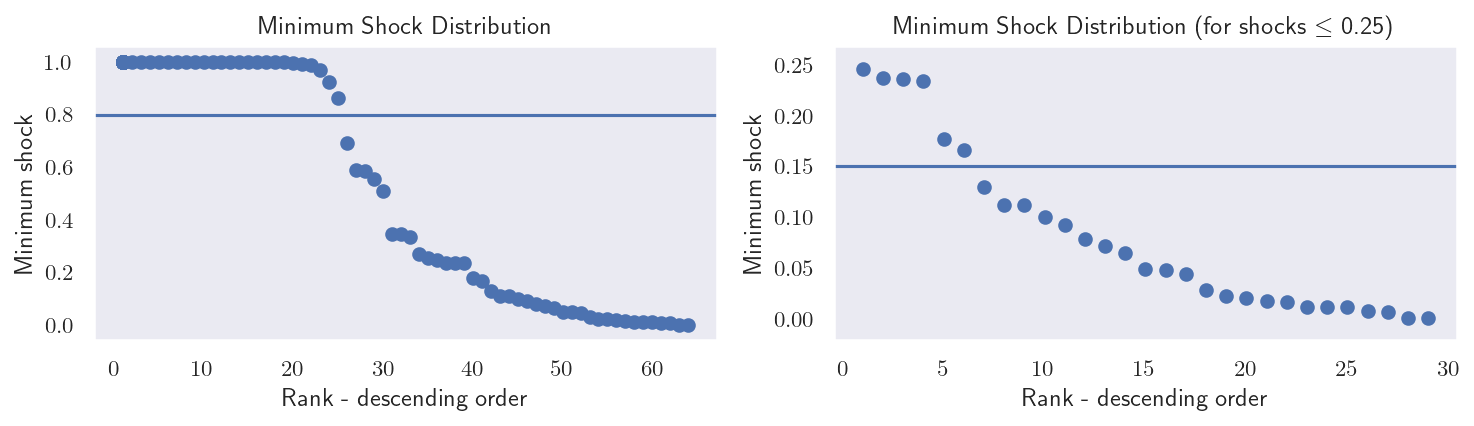
\includegraphics[width=\textwidth]{Fig522-MinimumShock.png}
		\caption{Minimum shock  distribution for the 2017 integrated circuit trade network }\label{fig:522MinimumShock}
	\end{figure}
	
	From Figure \ref{fig:522MinimumShock}, we find a clear gap between the minimum shock values for core and peripheral nodes. We set a threshold value of 0.8 to distinguish between these two groups.
	
	Once again, we end up with the same problem as before: a largely heterogeneous core. Thus, in search of a more homogeneous core, we drill down on the values and check for significant gaps.
	
	In doing so, we find from figure \ref{fig:522MinimumShock} a significant gap at a shock value of around 0.15. This is an order of magnitude greater than the threshold we set in the first agent-based simulation. Comparing the in-eigenvector distribution to the out-eigenvector distribution in Figure \ref{fig:512EigenvectorDistribution}, we see that there are less outliers in the former than in the latter. Thus, the network comprised of only the incoming links is more stable than that comprised of only outgoing links. As such, we need larger perturbations in this network to drive the simulation to termination.
	
	With our thresholds in place, we can 
	now divide the network into inner core, outer core and peripheral nodes, as before. We visualize the geographic distribution of core and peripheral nodes using a choropleth map.
	
	\begin{figure}[!h]
		\centering
		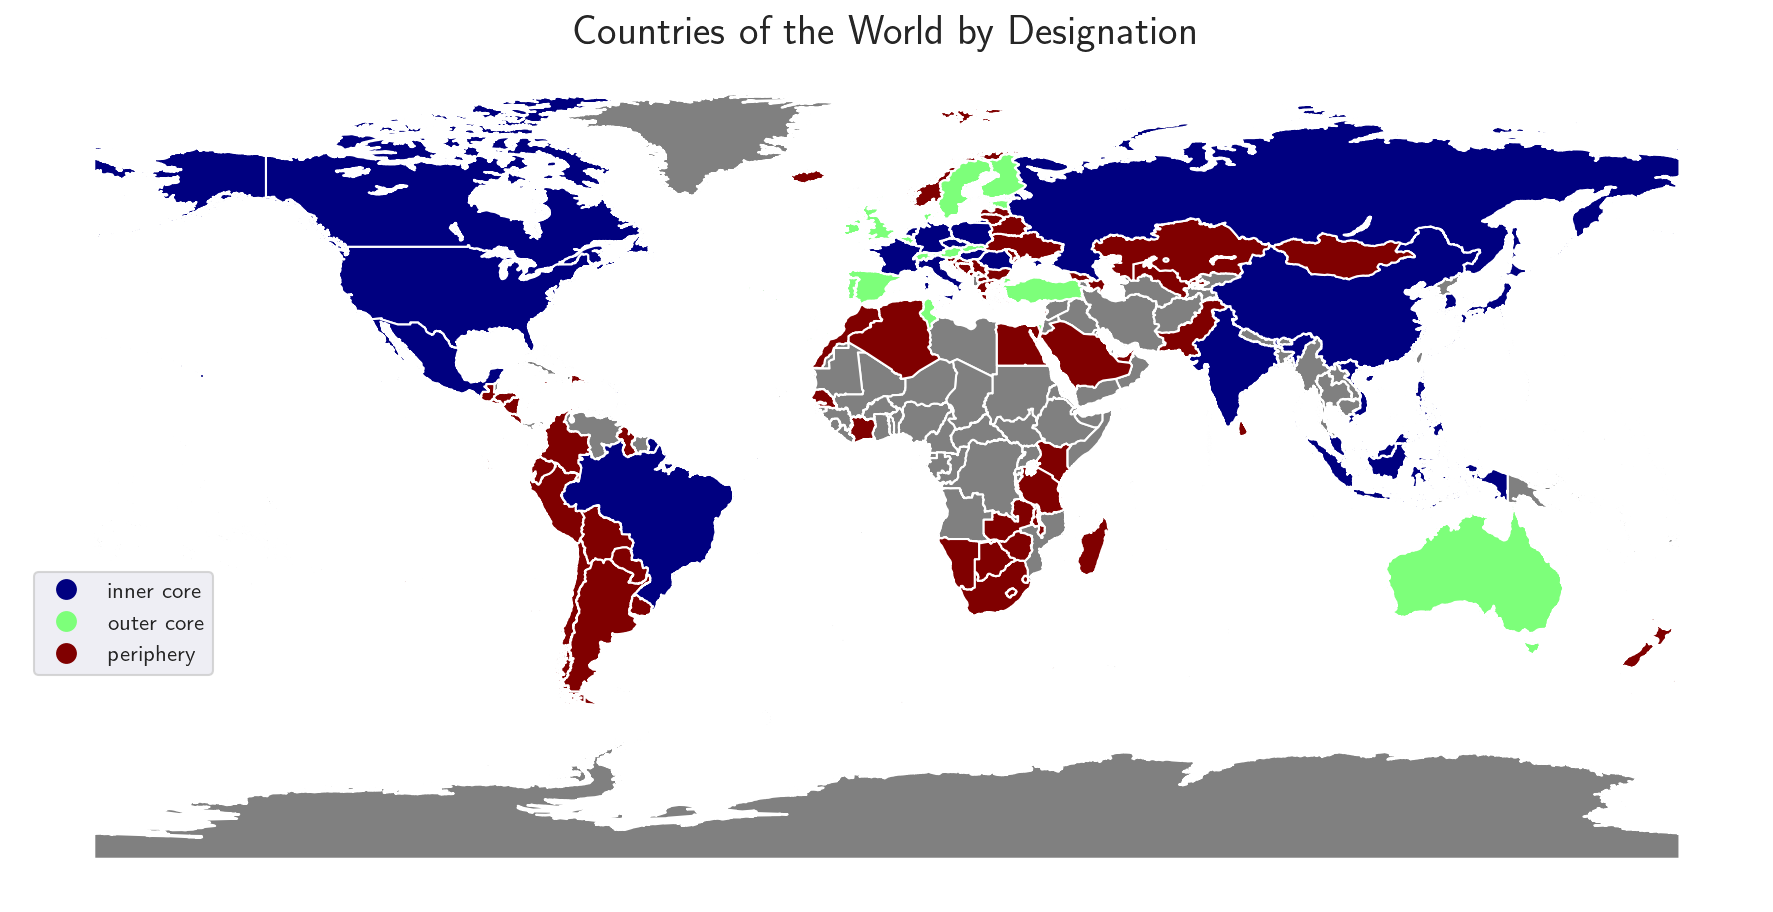
\includegraphics[width=\textwidth]{Fig523-CorePeripheryMap.png}
		\caption{Core-periphery map for the 2017 integrated circuit trade network}\label{fig:521CorePeripheryMap}
	\end{figure}
	
	Once again, we find from Figure \ref{fig:521CorePeripheryMap} that with respect to this agent-based simulation, the Southeast Asian/East Asian region is a major hub in the IC trade network. Other inner core regions include North America, Western Europe, Poland, Hungary, Romania, Brazil, Russia and India. As such, these regions are the most susceptible to systemic risk pertinent to events which are related to a supply-side increase. The periphery in this network is also much larger than that for the network of outgoing nodes, thus supporting our earlier conclusion that this network is more stable.
	
	Core-periphery networks are often characterized by (1) highly central core nodes and sparsely connected peripheral nodes and (2) a significant number of core-core and core-periphery links as opposed to periphery-periphery links. We examine if this is the case with the inner core, outer core and periphery.
	
	To determine whether this holds in our network, we look at the following metrics. To test the first assumption, we examine: (1) average in-degree centrality, (2) average in-strength centrality, (3) average betweenness centrality and (4) average in-eigenvector centrality. For the second assumption, we look at: (1) average link weight and (2) normalized number of links.

	\begin{longtable}{|l|r|r|r|r|}
		\caption{Average centrality based on designation. \label{tab:tab08AverageCentrality}} \\
		\hline
		& \textbf{\small in-degree} & \textbf{\small in-strength} & \textbf{\small betweenness} &
		\textbf{\small in-eigenvector} \\ 
		\hline
		\endfirsthead
		\hline
		& \textbf{\small in-degree} & \textbf{\small in-strength} & \textbf{\small betweenness} &
		\textbf{\small in-eigenvector} \\ 
		\hline
		\endhead
		\hline
		\endfoot
		inner core & 22.2608695652 & 0.0423048898 & 0.0749707764 & 0.0867081455 \\
		outer core & 19.2500000000 & 0.0013494807 & 0.0119492158 & 0.0059744019 \\
		peripheral & 7.3787878788 & 0.0000817552 & 0.0027977686 & 0.0006139597 \\
	\end{longtable}
	
	From Table \ref{tab:tab08AverageCentrality}, we find that inner core nodes tend to be associated with significantly higher in-degrees, higher in-strength centralities, higher betweenness centralities and higher in-eigenvector centralities relative to the peripheral nodes. However, the difference between the average centrality measures of the inner core and outer core nodes do not differ as significantly as in the earlier simulation. Again, this is due to the network of incoming links being more stable than the network of outgoing links.
	
	\begin{longtable}{|l|l|r|r|}
		\caption{Edge-level metrics based on designation. \label{tab:tab09EdgeLevel}} \\
		\hline
		\multicolumn{1}{|c|}{\textbf{\small source}} & \multicolumn{1}{|c|}{\textbf{\small target}} & \multicolumn{1}{|c|}{\textbf{\small average}} & \textbf{\small normalized number} \\ 
		\multicolumn{1}{|c|}{\textbf{\small designation}} & \multicolumn{1}{|c|}{\textbf{\small designation}} & \multicolumn{1}{|c|}{\textbf{\small link weight}} & \multicolumn{1}{|c|}{\textbf{\small of links}} \\ 
		\hline
		\endfirsthead
		\hline
		\multicolumn{1}{|c|}{\textbf{\small source}} & \multicolumn{1}{|c|}{\textbf{\small target}} & \multicolumn{1}{|c|}{\textbf{\small average}} & \textbf{\small normalized number} \\ 
		\multicolumn{1}{|c|}{\textbf{\small designation}} & \multicolumn{1}{|c|}{\textbf{\small designation}} & \multicolumn{1}{|c|}{\textbf{\small link weight}} & \multicolumn{1}{|c|}{\textbf{\small of links}} \\ 
		\hline
		\endhead
		\hline
		\endfoot
		inner core & inner core & 966725813.6482058764 & 0.4881422925 \\
		outer core & inner core & 68398425.7554181963 & 0.4510869565 \\
		peripheral & inner core & 9630549.9724778105 & 0.1739130435 \\
		inner core & outer core & 30874552.0952311717 & 0.4456521739 \\
		outer core & outer core & 4832637.2390983915 & 0.4166666667 \\
		peripheral & outer core & 570717.4141119211 & 0.0416666667 \\
		inner core & peripheral & 4285006.1312021175 & 0.3478260870 \\
		outer core & peripheral & 1151056.7283702765 & 0.1429924242 \\
		peripheral & peripheral & 599039.6658264966 &  	0.0597826087 \\
	\end{longtable}
	
	From Table \ref{tab:tab09EdgeLevel}, we find that inner core-inner core links tend to have significantly higher weights on average compared to the rest. Moreover, inter-inner core links tend to be much more frequent, with around 48\% of all possible core-core links actually in the network. Furthermore, as with the earlier result, the inner core-outer core-periphery hierarchy is not as obvious here as it had been in the results of the earlier simulation, due to the network of incoming links being more stable.
	
	\subsection{Exposure}
	\label{ssec:542exposure}
	
	\begin{longtable}{|l|l|r|l|l|r|}
		\caption{Top countries in terms of exposure with respect to the Philippines for the 2017 integrated circuit trade network. \label{tab:tab10Exposure2}} \\
		\hline
		\textbf{\small Rank} & \textbf{\small Country} & \multicolumn{1}{|c|}{\textbf{\small Exposure}} & \textbf{\small Rank} &
		\textbf{\small Country} & \multicolumn{1}{|c|}{\textbf{\small Exposure}} \\
		&  & \multicolumn{1}{|c|}{\textbf{\small given}} & & & \multicolumn{1}{|c|}{\textbf{\small received}} \\  
		\hline
		\endfirsthead
		\hline
		\textbf{\small Rank} & \textbf{\small Country} & \multicolumn{1}{|c|}{\textbf{\small Exposure}} & \textbf{\small Rank} &
		\textbf{\small Country} & \multicolumn{1}{|c|}{\textbf{\small Exposure}} \\
		&  & \multicolumn{1}{|c|}{\textbf{\small given}} & & & \multicolumn{1}{|c|}{\textbf{\small received}} \\  
		\hline
		\endhead
		\hline
		\endfoot
		1 & South Korea & 0.2168246753 & 1 & Singapore & 0.0882802430 \\
		2 & USA & 0.1519925691 & 2 & Germany & 0.0695426272 \\
		3 & Japan & 0.0836142176 & 3 & France & 0.0510759890 \\
		4 & Ireland & 0.0360864373 & 4 & The Netherlands & 0.0481932111 \\
		5 & Malaysia & 0.0292577817 & 5 & Malaysia & 0.0441913096 \\
		6 & Singapore & 0.0214444666 & 6 & Hungary & 0.0392266581 \\
		7 & Israel & 0.0070685452 & 7 & Poland & 0.0379054991 \\
		8 & Italy & 0.0067494026 & 8 & Hong Kong & 0.0338060255\\
		9 & Belgium & 0.0064295498 & 9 & Romania & 0.0334363579 \\
		10 & France & 0.0049168955 & 10 & Italy & 0.0330343353 \\
	\end{longtable}
	
	We find that the Philippines is affected by South Korea the most, with the country being exposed to 21.68\% of the shock from South Korea on average. Meanwhile, the Philippines affects Singapore the most, with the country being exposed to 8.82\% of the shocks from the Philippines on average.
	
	\section{Additional Remarks and Recommendations}
	\label{sec:55additionalRemarks}
	
	We plot the minimum shock values for both scenarios against the respective out- and in-centralities. This is because of the fact that a country's centrality may influence its importance 
	in the network with respect to the cascading failures model.
	
	\begin{figure}[!h]
		\centering
		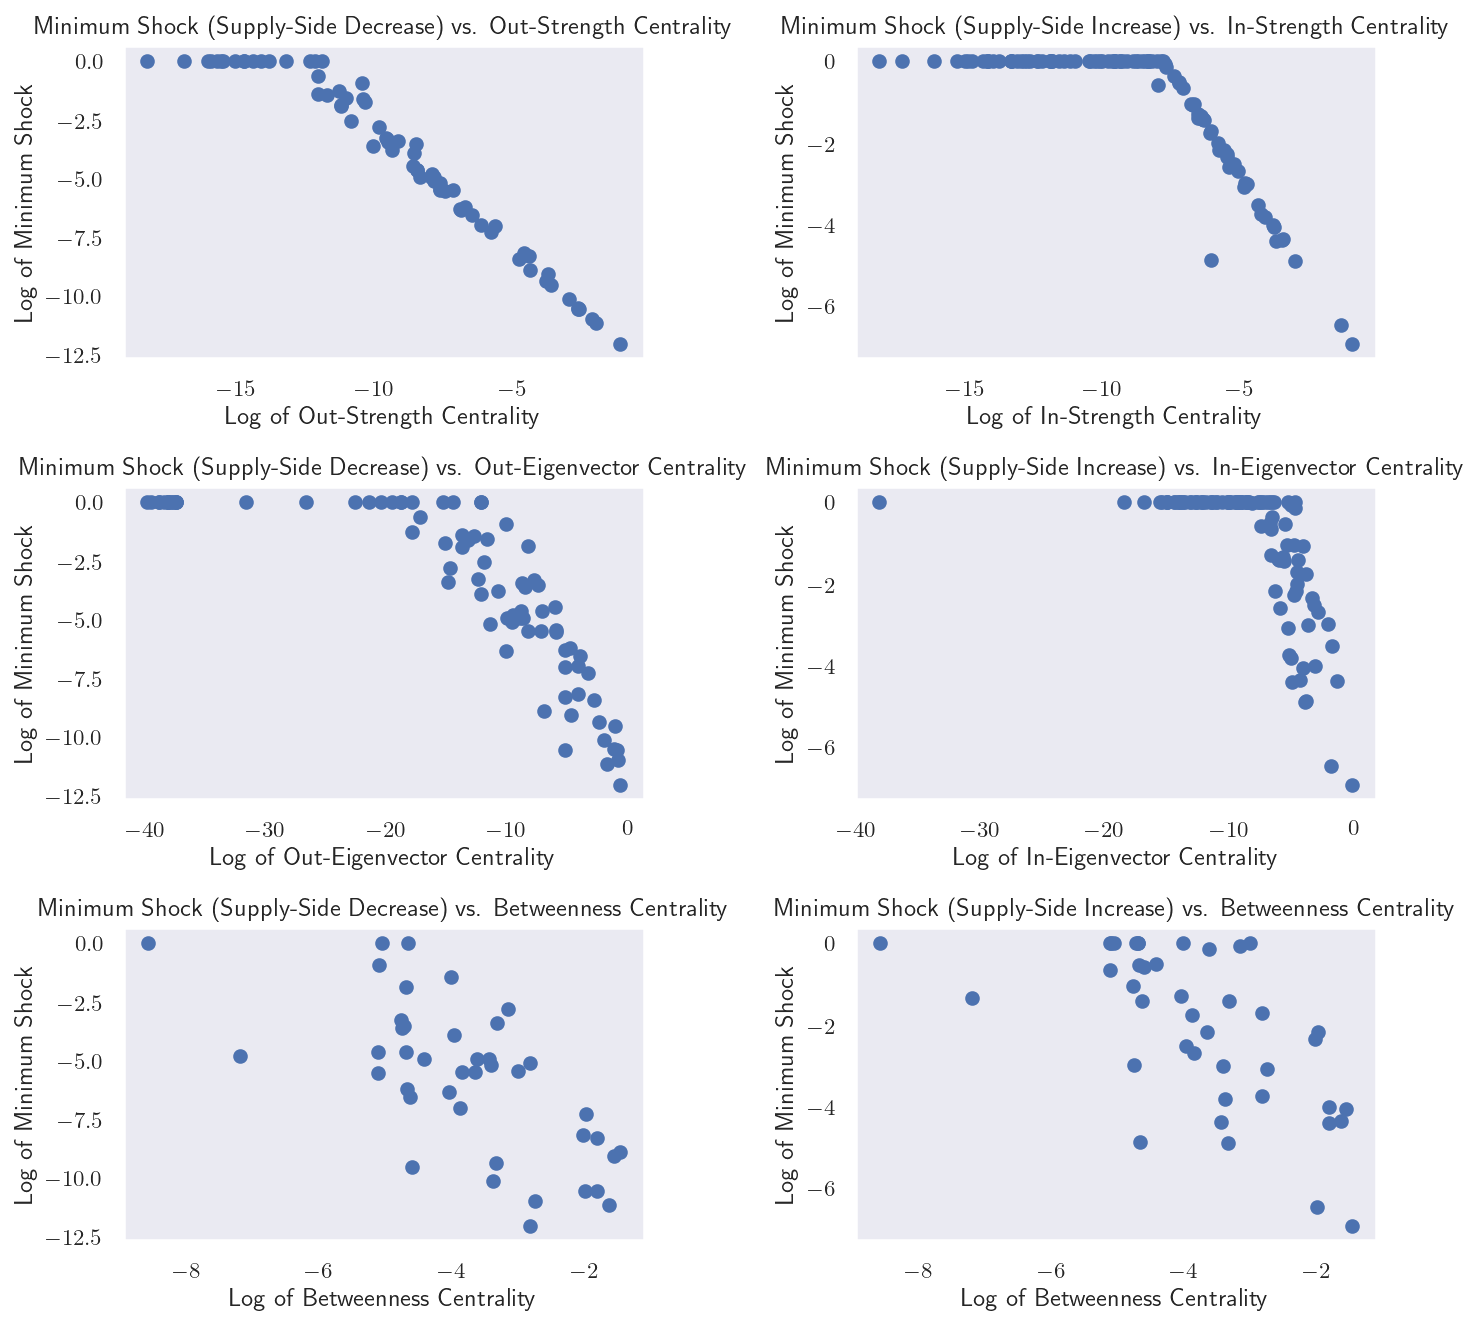
\includegraphics[width=\textwidth]{Fig524-ShockvsCentrality.png}
		\caption{Minimum shock vs. out- and in-centralities}\label{fig:523ShockvsCentrality}
	\end{figure}

	We find from the log plots in Figure \ref{fig:523ShockvsCentrality} that the relationship ranges from strongly linear to weakly linear. The relationship is strongly linear with respect to the strength centrality, moderately linear with respect to the eigenvector centrality and weakly linear with respect to the betweenness centrality. This suggests that the minimum shock is related to the centrality of a node through a power law.
	
	Furthermore, this suggests that trade volume is an important determinant of a country's systemic risk in the trade network, much more so than the relative importance of its trade partners or its position in the trade network. This is because in the context of our model, if a country has a high trade volume to relatively smaller countries (which themselves tend to have smaller imports/exports), a small supply-side perturbation can easily lead to the simulation terminating. On the other hand, having important neighbors or being in between important countries will not usually guarantee this, since the neighboring countries will themselves have relatively higher imports/exports. 
	
	As such, local importance is more important in the context of this model as opposed to global importance. This necessitates the formulation of a centrality measure which can account for a country's local importance in the trade network. 

	It is important to note here the limitations of our model. Since our simulation terminates once a node can no longer reduce its exports/imports, local connections become more important compared to global ones. In contrast, in the model by Li et al. (2014), the simulation continues despite the failure of any one node and terminates only when a certain percentage of nodes have failed. In such a model, global connections could potentially be more important as opposed to local ones, as the shock would not only have to be destructive but also pervasive. It would be interesting to see how our results would vary in light of such a change in our model.

	We can also note the buildup of nodes at around the zero mark of the y-axis, corresponding to the peripheral nodes in the network. It would be interesting to examine the role of $k_{max}$, the maximum number of iterations, as a limiting factor in this distribution. For the simulations, we assumed a value of 50 for $k_{max}$, meaning that the simulations were allowed to run for at most 50 iterations. This is done for computational efficiency. 
	
	Note from Figure \ref{fig:517CascadeSizevsDepth} and Figure \ref{fig:520CascadeSizevsDepth} that nodes "jump" from the periphery to the core upon modifying the shock and spread parameters. Were we to allow the simulation to run for a larger number of iterations, more nodes in the periphery could possibly make that "jump". One might want to extend $k_{max}$ to larger values and determine if the periphery we identified in this study is robust to increases in $k_{max}$. Of course, this would require significantly more computational power.

\chapter{Summary of Findings, Conclusions and Recommendations}
\label{chap:6Conclusion}

In Section 5.2, we found that the link density, total link weight and degree assortativity have largely been increasing over the years, primarily due to globalization. In particular, the increasing assortativity tells us that high-degree nodes have been forming more links with other high-degree nodes during the past few years. 

The agent-based simulations in Sections 5.3 and 5.4 revealed that the network of incoming and outgoing links both exhibit a core-periphery structure, with cascade depth as the distinguishing metric. That is, the IC trade networks are characterized by a highly central and well-connected core and a sparsely-connected periphery. As a result, there are more core-core and core-periphery links than there are periphery-periphery links. Peripheral networks can also be divided into connected and isolated nodes with cascade size as the distinguishing metric, although the distinction is markedly less important.

Furthermore, we found that there are three main (geographic) blocs for the IC network: North America, Western Europe and East/Southeast Asia. Both are core regions with respect to both the outgoing and incoming networks, suggesting that they have a significant midstream presence in the network. Notably, there are a number of countries which are only core countries with respect to the outgoing network (e.g., Spain, Portugal, Morocco, Sweden, Finland) and a number of countries which are only core countries with respect to the incoming network (e.g., Brazil, Russia, India).

As such, the three regions pose a significant systemic risk, as they are not only important exporters but are important importers as well. Any trade war, embargo or significant perturbation to the integrated circuit supply pertaining to these countries can significantly affect the rest of the countries in the IC network. 

Moreover, we found that the IC network is generally more resilient to supply-side increases than to supply-side decreases, as the network of incoming links is more stable than the network of outgoing links. 

Lastly, using the exposure metric in Sections 5.3 and 5.4, we found that the Philippines is primarily susceptible to shocks from the Southeast Asian/East Asian region. Conversely, countries in the Southeast Asian/East Asian region are also susceptible to shocks in the Philippines.

In addition to the recommendations put forth in Section 5.5, further studies can work towards relaxing the assumptions that are implicit in the model. For one, the agent-based model in the paper uses two global parameters: the shock and spread parameter. One of the appealing features of network-based modelling, however, is that we are able to heterogenize the actions of the agents in the network, in effect accounting for differences in how different classes of nodes would respond to shocks. 

In particular, the location of a country in the global value chain can affect how it responds to an economic shock. A supply-side decrease could potentially affect countries that are more downstream in the value chain, for example, as opposed to those that are more upstream in the value chain. Using the methodology outlined in Cingolani, Panzarasa \& Tajoli (2017), one can quantify a country's upstreamness, downstreamness and midstreamness in the integrated circuit value chain and can use these measures to parametrize different behaviors for upstream, midstream and downstream countries.

Another example would be the difference in behavior between wealthy and poor countries, which was parametrized by Gephart et al. (2016). Richer countries may be able to weather the higher prices brought about by a decreased supply, so they receive more of the shock. The demand of poorer countries, however, is more elastic, and so they receive less of the shock. We can calibrate our agent-based model to take all these differences into account, resulting in a more realistic model.

Furthermore, we make the simplifying assumption that the model terminates when one of the nodes fails – that is, if one of the nodes can no longer reduce its exports/imports. In truth, however, the other nodes can continue exporting, independent of any other nodes' failure. We can in fact extend the model by allowing it to continue past the failure of any one node and calculating the minimum shock parameter needed to bring about the failure of a certain percentage of the nodes in the network, as in Li et al. (2014).

Moreover, the assumption on the time scale of the shocks can be relaxed to accommodate more complex scenarios. We can make the time scales dependent on the countries, for example, and introduce some lag for particular countries based on their openness to imports/exports. \cite{losercs224w}

The model also proves itself timely with the current COVID-19 pandemic. The World Customs Organization and the World Health Organization have jointly released the commodity classifications of different product categories which have been deemed essential in light of the current situation. In addition, many countries have been found to be in dire need of these medical supplies, constituting a demand-side increase. The model can be extended to accommodate for these scenarios and to ultimately determine how these can affect the trade network as a whole. 

We can still employ our current model for particular scenarios, however. For instance, certain countries have restricted trade on important supplies such as face masks to better service their domestic population, which constitutes a supply-side decrease.

In conclusion, using simple agent-based modelling, we were able to determine that a core-periphery structure exists in both the network of outgoing and incoming links in the integrated circuit trade network. More importantly, we determined that the Southeast Asian/East Asian region (and by extension, the Philippines) have a notable midstream presence in the network.

\nocite{*}

	\begin{appendices}
	\addtocontents{toc}{\cftpagenumbersoff{section}}
		\chapter{Python Script}
		\lstinputlisting{MANAY_THESIS_CODE.py}
	\end{appendices}

\bibliography{thsphyref}
\end{document}          